%\documentclass[a4paper, 10pt]{IEEEtran}      % for icra/RAL final
\documentclass[usletter, 10pt, conference]{ieeeconf} % initial submission to RAL/ICRA
\usepackage{graphicx}
\usepackage{booktabs}
%\usepackage{amsmath}
\usepackage{amsfonts}
\usepackage{subfig}
\usepackage[ruled,lined]{algorithm2e}
\usepackage{multirow}
\usepackage{flushend}
\usepackage[bookmarks=false]{hyperref}
\usepackage{setspace} % for setstretch in algorithm
\pdfminorversion=4

\IEEEoverridecommandlockouts                              % This command is only
\overrideIEEEmargins


\newcommand{\red}[1]{\textcolor{red}{#1}}
\newcommand{\tylde}{$\sim$}

%\hypersetup{colorlinks=true,linkcolor=black,citecolor=black}

\SetKwInput{KwData}{Global params.}

\title{Motion planning for assessing accessibility of protein tunnels}

\author{Vojt\v ech Von\' asek$^{1}$,
    Barbora Kozl\'\i kov\'a$^{2}$,
    Adam Jur\v{c}\'\i k$^{2}$,
    Martin Saska$^{1}$
\thanks{$^{1}$ Faculty of Electrical Engineering,  Czech Technical University in Prague, 
Technick\'a 2, 166 27 Prague, Czech Republic,
{\tt vonasek@labe.felk.cvut.cz}}
\thanks{$^{2}$        
Faculty of Informatics,   Masaryk University, Botanick\'a 68a, 602~00 Brno, Czech Republic,
%The presented work has been supported by the Czech Science Foundation (GA{\v C}R) under research project No. 17-07690S.
%Access to computing and storage facilities owned by parties and projects contributing to the National Grid Infrastructure MetaCentrum, provided under the programme "Projects of Large Infrastructure for Research, Development, and Innovations" (LM2010005), is greatly appreciated.
%}%
}
}


%D. Bedn\'{a}\v{r}:
%Faculty of Science, Masaryk University, Kamenice 5, 625 00 Brno, Czech Republic\\


\def\qrand{q_{rand}}
\def\qstart{q_{start}}
\def\qinit{\qstart}
\def\qgoal{q_{goal}}
\def\qnear{q_{near}}
\def\qnew{q_{new}}
\def\T{\mathcal{T}}

\def\C{\mathcal{C}}
\def\CF{\mathcal{C}_{free}}
\def\CFD{{\mathcal{C}^s_{free}}}
\def\dt{d_{tunnel}}
\def\da{d_{atom}}
\def\R{\mathbb{R}}
\def\QI{Q_{init}}
\def\RI{R_{init}}

\def\rv{R_{tunnel}}


\def\Imax{I_{max}} %max number of iterations of RRT-based planners

\def\dist{\mathrm{dist}}
\def\dists{\mathrm{dist}_{\mathrm{s}}}

\SetKw{return}{return}

\def\smin{s_{min}}
\def\smax{s_{max}}
\def\sdelta{s_{\Delta}}


\def\probe{r_{\mathrm{probe}}}
\def\Sprobe{S_{\mathrm{probe}}}

\def\gprobe{r_{\mathrm{out}}}
\def\Sgprobe{S_{\mathrm{out}}}


\def\CG{\mathcal{C}_{goal}}
\def\SB{\mathbf{S}_{blocking}}
\def\SS{\mathbf{S}}


%spacing for algorithm environment. 1.0 mean normal spacing
\def\gb{p_{tunnel}}

\def\L{\mathcal{L}}
\def\S{\mathcal{S}}

\def\LA{L_1}
\def\LB{L_2}

\def\RA{A$_{1}$}
\def\RB{A$_{2}$}


% ==================================================================================

\begin{document}

\maketitle
\thispagestyle{empty}
\pagestyle{empty}

\begin{abstract}
Chemical interactions between proteins and other molecules (ligands) take place in specific locations, called active sites, that are often deeply buried inside the protein structure.
These active sites are accessible through one or more void paths, called tunnels.
Nowadays, tunnels are mostly computed using Voronoi diagrams which approximate the ligand by a bounding sphere.
This leads to highly imprecise results.
To address this problem, we define the computation of the transportation path of non-spherical ligands including their conformation changes (i.e., when the atoms of the ligand move relatively to each other) as a motion planning task in high-dimensional configuration space.
This can be solved using sampling-based planning methods.
We propose a modification of the Rapidly Exploring Random Tree planner for the purpose of trajectory computations of flexible ligands.
To cope with the narrow passage problem, the random samples are generated around a Voronoi-based tunnel, which serves us for better localization of the searched space.
The flexibility of the ligand is modeled using a fixed set of known conformations, which does not increase the number of dimensions of the configuration space.
The proposed method has been evaluated in a virtual screening scenario to estimate the traversability of tunnels for several ligands.
\end{abstract}


\section{Introduction \& Motivation}


Reactivity of proteins with other molecules plays a crucial role in many research disciplines, including protein engineering and drug design.
Protein reactivity is tightly connected with the presence of the void space between its amino acids. 
This space, forming a path called tunnel, can be utilized by a small molecule (ligand) which can enter the protein inner space and react with its amino acids surrounding a specific site, called the active site~\cite{gora2013gates}.
The size and location of tunnels determine the ligand size and shape which can enter the active site.
%The tunnel has to be wide enough and also the physico-chemical properties of the surrounding amino acids have to be compatible with the ligand.
Biochemists are currently using computational methods for tunnel detection in order to estimate the possibility of interactions between a protein and a ligand without the need to perform laboratory experiments (Fig.~\ref{fig::motiv}).
The most common methods detect tunnels using Voronoi diagrams~\cite{yaffe2008,caver3} assuming a spherical ligand (probe), i.e., the ligand is approximated by a bounding sphere.
However, as the ligands are typically non-spherical and flexible, these methods can often skip possible candidate tunnels.

\begin{figure}[t]
\centering
{\footnotesize
\renewcommand{\arraystretch}{-0.5}
\renewcommand{\tabcolsep}{-1pt}
\begin{tabular}{ccc}
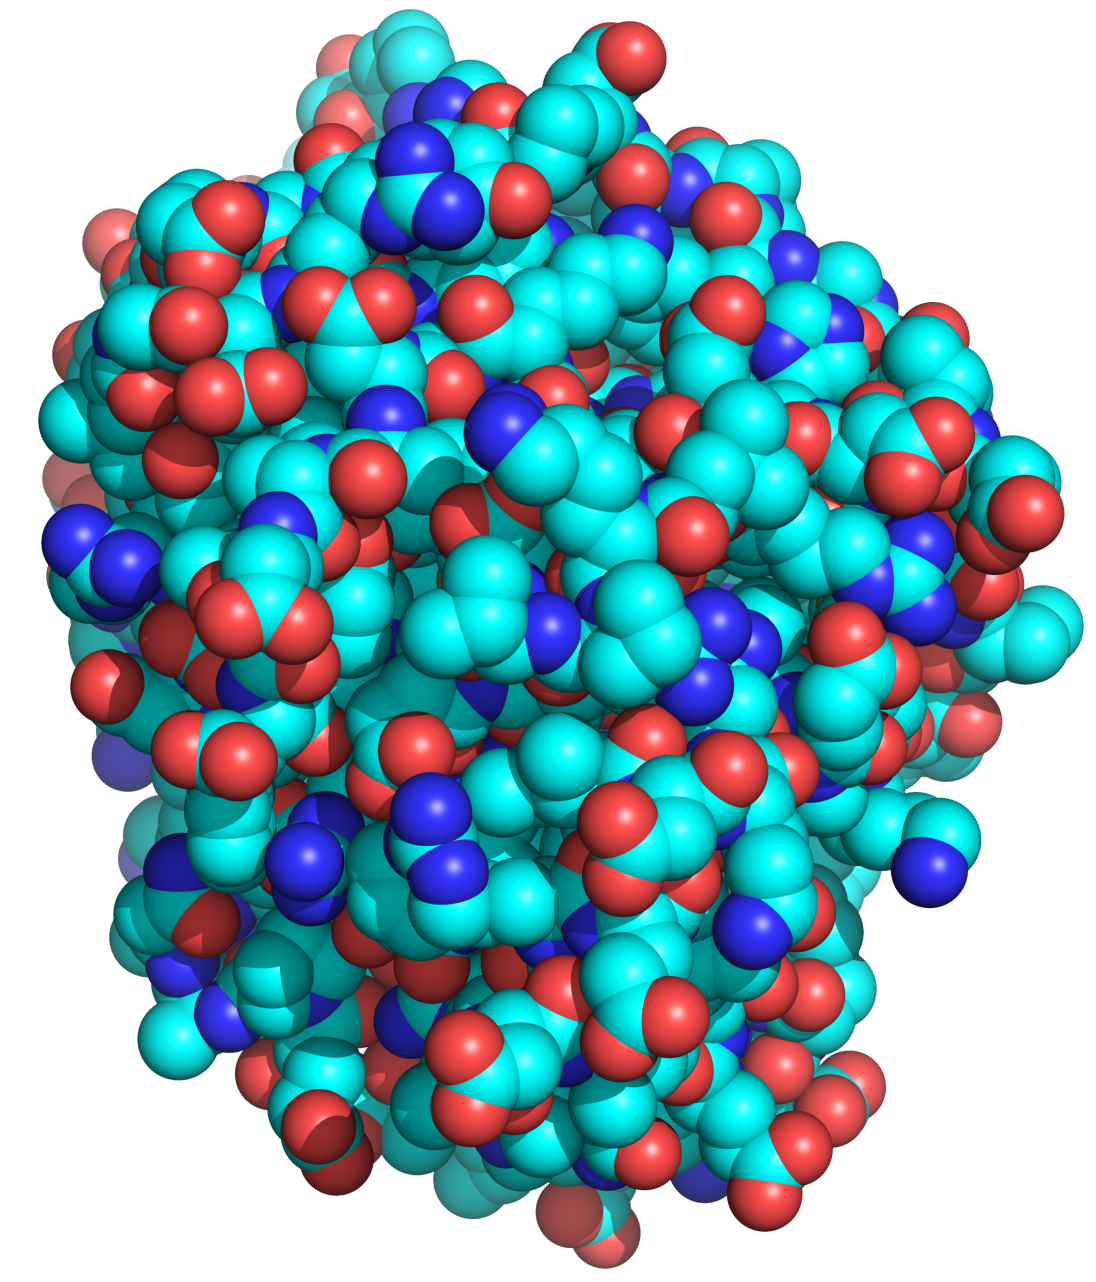
\includegraphics[width=0.15\textwidth]{fig/motiv1} &
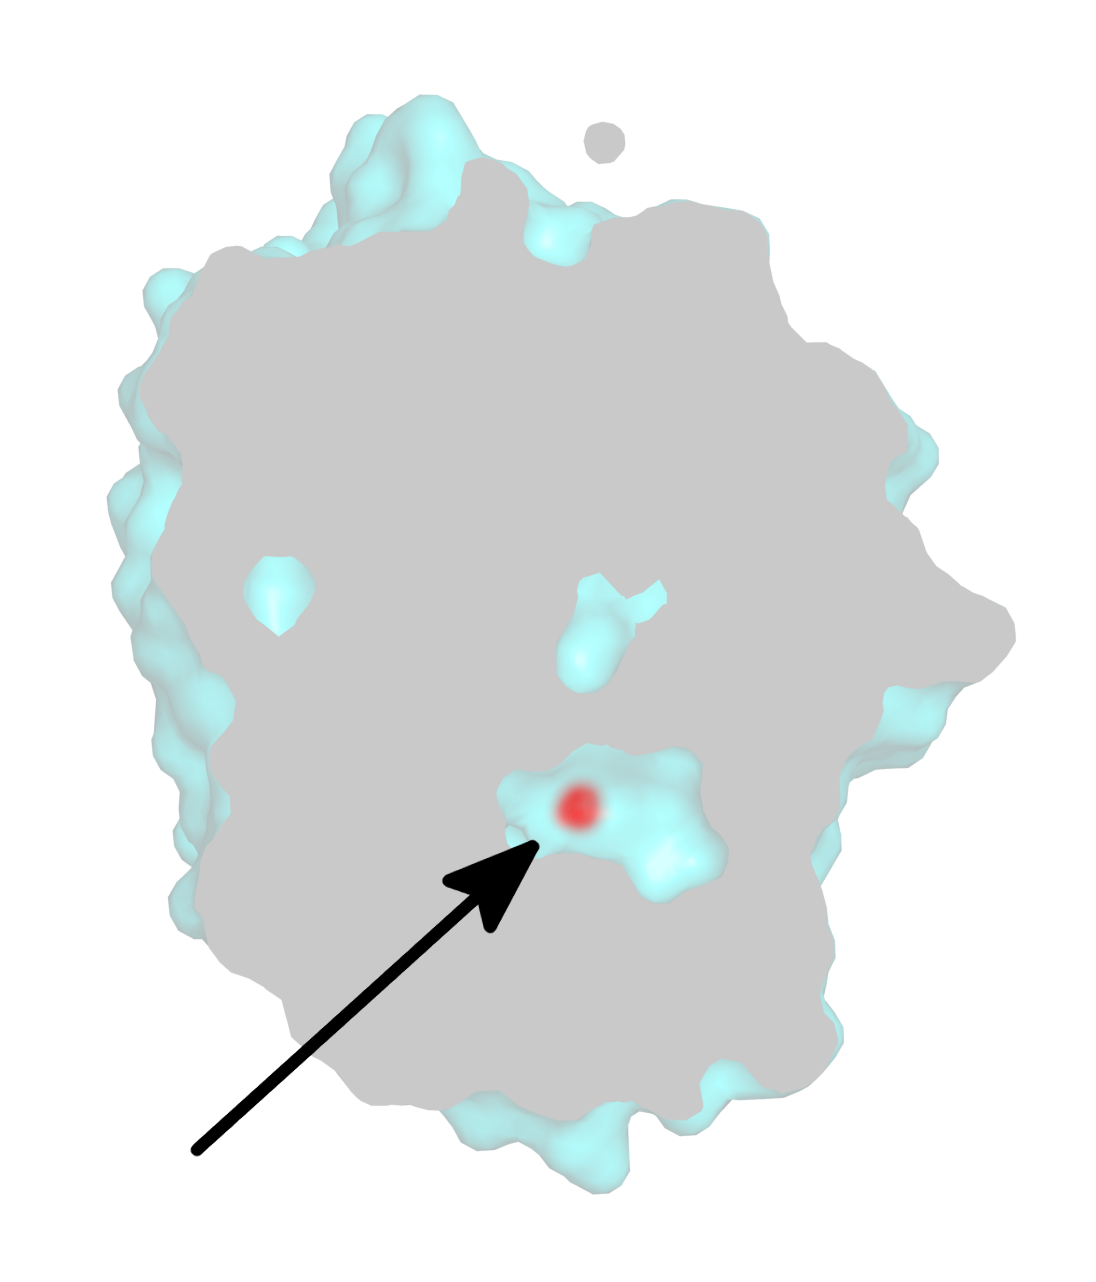
\includegraphics[width=0.17\textwidth]{fig/motiv2lab} &
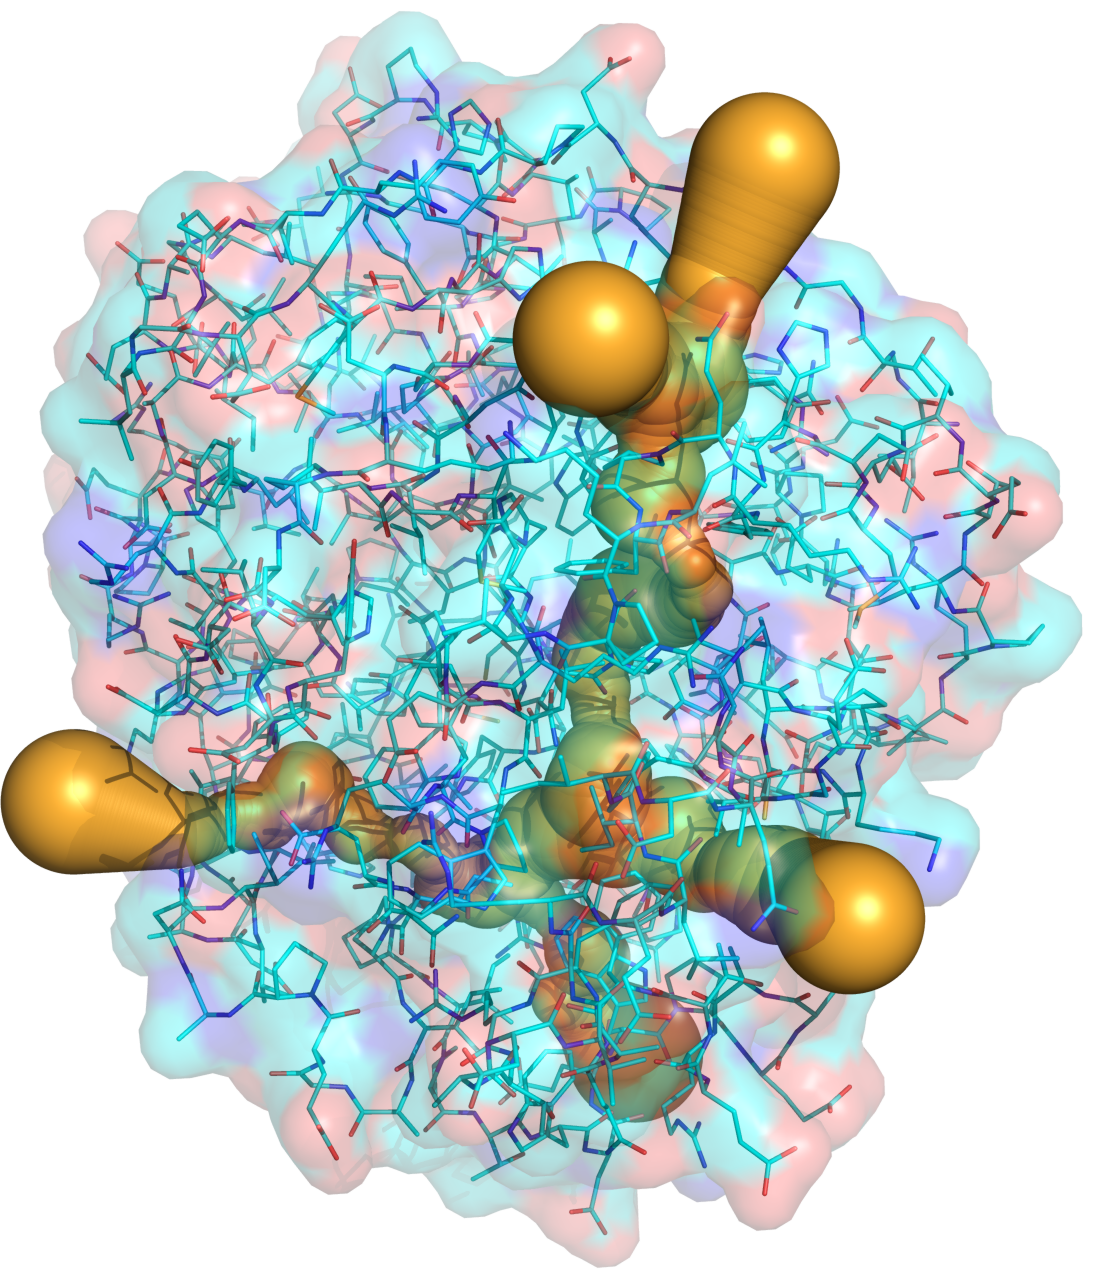
\includegraphics[width=0.16\textwidth]{fig/motiv3}  \\
Protein 1CQW & Active site & Detected tunnels \\ %& Example of a  \\
             &            & (orange)         \\  %& trajectory
\multicolumn{3}{c}{%
\includegraphics[width=0.16\textwidth]{fig/renderDCP}  \hskip 15pt
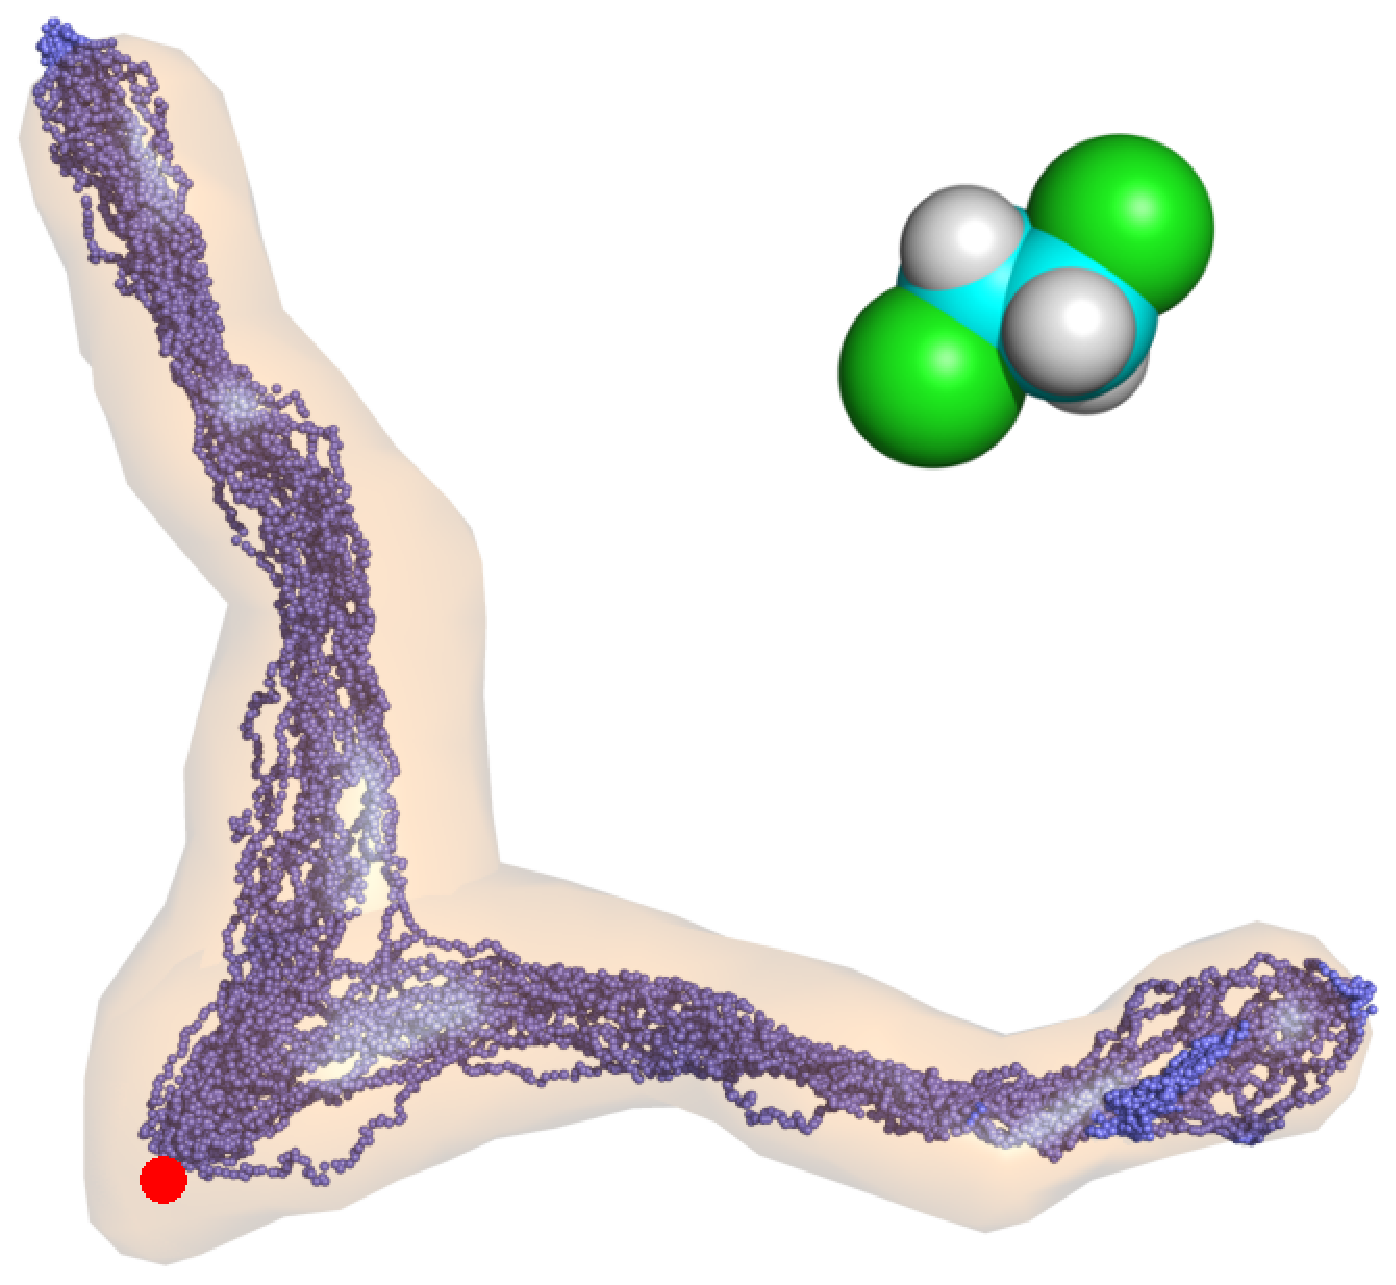
\includegraphics[width=0.14\textwidth]{fig/render37t}} \\ 
%\hbox{
%\vbox{
%\hbox{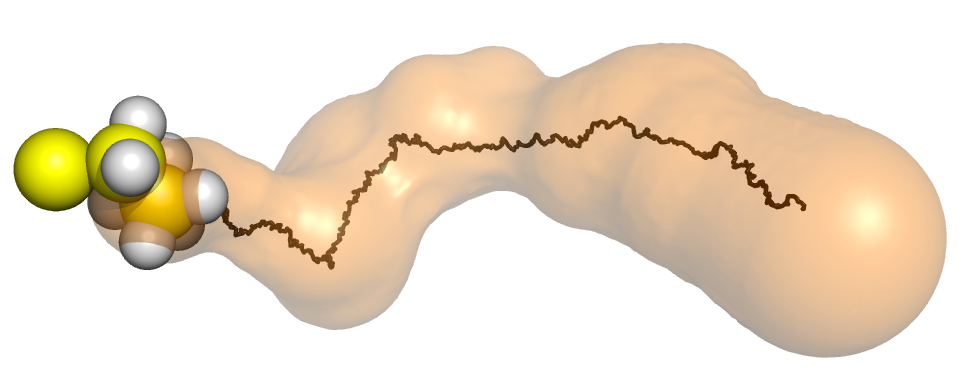
\includegraphics[width=0.25\textwidth]{fig/ta-1} }
%\hbox{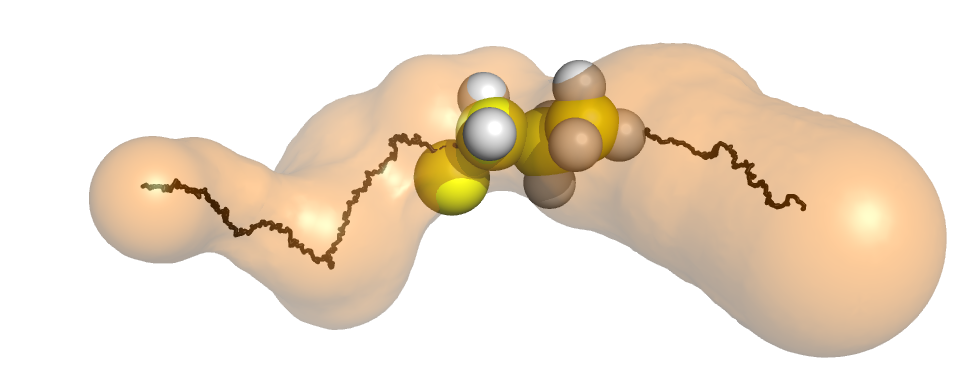
\includegraphics[width=0.25\textwidth]{fig/ta-433}}
%} 
%}
\end{tabular}
}
\caption{\label{fig::motiv}
    Tunnels in the DhaA haloalkane dehalogenase protein (PDB ID 1CQW) with possible trajectories of 1-Chlorpropan ligand (bottom left) and 1,2-Dichloroethane (bottom right).
}
\end{figure}


To provide the biochemists with a solution which detects also candidate tunnels omitted by the traditional methods, it is necessary take into account also the ligand shape and its conformation changes when the ligand moves, i.e., changes its conformation.
Such a ligand changing the mutual position of its atoms within a molecular dynamics is denoted as a flexible ligand.
To address this, we can formulate the task as a motion planning problem.
It is also necessary to cope with the narrow passage problem, as the proteins are dense structures and the movements of the ligand are limited by the surrounding amino acids.

The idea of the sampling-based motion planning is to randomly sample the configuration space of the robot and to connect the collision-free samples
into a graph structure (roadmap).
A path in the roadmap then corresponds to a motion in the workspace.
%The random samples are classified as free or non-free using black-box collision detection which allows the sampling-based methods to find paths for robots of various shapes. 
%The sampling-based planners can cope with robots with many degrees of freedom (DOF).
Two most commonly used sampling-based techniques are Probabilistic Roadmaps (PRM)~\cite{kavrakiForPP} and Rapidly Exploring Random Trees (RRT)~\cite{lavalleRRT}.
The sampling-based planners can cope with many-DOF (Degrees of Freedom) robots of an arbitrary shape.
Therefore, they have been used for motion planning of various robotic systems.
Besides many applications in robotics, the sampling-based planners have been already used in biochemistry as well 
%Sampling-based motion planners has been intensively studied in robotics, but they have been applied also in other research fields.
%In bio-chemistry, the planners have been used to study
to study loop motions~\cite{cortes2004geometric}
%protein folding~\cite{amato2002using,raveh2009rapid,novinskaya2015improving,songPFintro},
and for protein folding~\cite{raveh2009rapid,novinskaya2015improving}.
%or for tunnel detection~\cite{vonasek2017tunnel}.

In this paper, we propose a modification to RRT to address the problem of planning a non-spherical flexible ligand passage through a given protein.
We localize the generation of the random samples, i.e., instead of sampling the whole configuration space we focus only on the space surrounding a potential tunnel detected by the Voronoi-based method (using a smaller ligand probe in order to avoid omitting possibly feasible tunnel candidates).
The potential tunnel is represented by a set of consecutive spheres surrounding the tunnel centerline.
This optimization allows us to find trajectories along the given tunnel, which is faster than searching for any trajectory in the whole protein.
To enable the movement of the ligand in the narrow parts of the tunnel, the free-space can be dilated by shrinking the atom radii, similarly, e.g., to~\cite{cortes2005path,hsu06multilevel}. 
The ligand flexibility is modeled using a fixed set of predefined configurations which the ligand can occupy.

Our proposed method was tested by the biochemists who compared the results with trajectories of ligands determined experimentally in the lab.

%or protein folding combined with ligand diffusion~\cite{cortes2010simulating}.
%rrt for molecular: \cite{al2012motion}
%survey \cite{gipson2012computational}
%Sampling-based planners have been used in various applications in robotics~\cite{elbanhawi2014sampling} and also  %,latombe1999motion} and also
%Solutions for tunnel detection using sampling-based methods however have not been discussed yet.
%Understanding of interactions between proteins and other small molecules is crucial in many research fields, including drug design and protein engineering. 
%The knowledge about the existence of the tunnels and their properties (e.g., their bottleneck and chemical properties around the tunnel),
%is important to understand interactions between proteins and other molecules (ligands)~\cite{Koudelakova2013}.
%As the interaction takes place in the active site, the existence of a tunnel connecting the active site with the outer environment
%is necessary for the interaction.
%To get the ligand to the active site, a transportation tunnel connecting the protein outer environment with the active site has to exists.
%Biochemists decide if a tunnel can be used to transport a given ligand mainly based on the tunnel length and bottleneck (i.e., the radius of the smallest sphere that forms the tunnel).
%This is used for example in protein engineering, where the task is to change selected properties of a protein, e.g., its stability under different outer conditions~\cite{Koudelakova2013}. % or its activity of the protein towards other molecules~\cite{Pavlova2009}.
%The design of suitable ligands causing the desired changes can be speeded up by detecting and analyzing the tunnels leading to the active sites.
%This can be achieved by detecting and studying so called tunnels in proteins which can serve as the transportation paths for the 
%ligand from the outside environment to the active site or vice versa. 
%Whereas the tunnel computation is already a well established research field, the simulation of ligand transportation through the detected tunnels is rather new.
%Ligands are typically of non-spherical shape, therefore it is difficult to estimate their traversability through tunnels computed for a spherical probe.
%The decision based only on spherical tunnels requires previous expertise in the domain and yet it may be imprecise.

%Proteins are dense structures which limits movements of the ligand insider the tunnels, which leads to the narrow passage problem.
%To cope with this problem, we propose to utilize the principle of guided sampling~\cite{vonasek2009rrt,denny2016dynamic}.
%It helps to keep also potential solutions which do not fit to the geometric restrains but can be still feasible because of the physico-chemical properties.
%This strategy helps to overcome the limitations of the conformational discretation introduced by the rotamer approximation.

%The proposed method can be seen as an extension for the traditionally used tunnel detection tools.
%Besides trajectory computation, visualization of the results in important. %we also propose methods for their visualization.
%Our motivation is to help the biochemists to perform so called virtual screening, where they test the traversability of a ligand through a given tunnel.
%In order to predict the success of ligand traversability, the virtual screening performs hundreds of thousands of tests and checks if the ligand passed through the tunnel.
%The advantage of the proposed approach is that we can search the ligand path inside a specific tunnel which substantially decreases the computational time and resources required for the virtual screening.
%We further propose visualization techniques for presenting the results to biochemists.
%Therefore, methods for visualization of the results  are discussed.

\section{Related Work}

%The analysis of protein structure aiming to reveal the tunnels has been supported by different computational software tools which take the geometry of the protein as an input and explore the inner void space (e.g., CAVER 1.0~\cite{petrek2006caver} or MOLE~\cite{Petrek20071357}). 
%Early methods for tunnel detection utilized a discretized 3D grid, where each cell is considered as occupied or free depending
%on the presence of atoms of the protein~\cite{petrek2006caver,Petrek20071357}.

%TODO some words about MD and why it better to analyze stuff with tunnels than with MD


Most of the available tools for tunnel detection are based on Voronoi diagrams~\cite{yaffe2008,caver3} or they utilize a grid-based computation~\cite{sehnal2013mole}.
%The tunnels are pathways computed for a single atom (spherical probe) using Voronio-diagrams~\cite{yaffe2008,caver3} or 
%grid-based approaches~\cite{sehnal2013mole,petrek2006caver}.
The resulting tunnels are represented as a sequence of spheres and characterized by their bottleneck, length, curvature, and a list of surrounding residues, whose physico-chemical properties are crucial for assessing the interaction possibilities between the protein and ligand.
More details can be found in the recently published state-of-the-art report about analysis and visualization of biomolecular cavities~\cite{Krone_2016}.
The main disadvantage of both grid-based and VD-based methods is that the shape of the ligand is not taken into account during the tunnel detection and it is therefore not easy to estimate if (and how) a non-spherical ligand might traverse the tunnel.
Moreover, the ligand flexibility cannot be principally considered by these approaches.
Simulations based on molecular dynamics (MD) can directly evaluate migration of a ligand into a protein, but they are significantly more computationally demanding~\cite{kingsley2014including}. 
Moreover, MD simulations have to be prepared for a specific ligand/protein pair, which is not practical for testing a large number of ligands.
The geometric-based methods are therefore still preferable due to their fast speed.
In order to determine if the ligand can pass the tunnel using the geometric-based methods, it is necessary to compute a trajectory considering the shape of the ligand and its 3D translation and rotation.

%This can be formulated as a motion planning problem in a high-dimensional configuration space $\C$.
%In this case, the configuration space $\C$ has at least $6+n$ dimensions (3D rotation + 3D translation + additional degrees of freedom
%caused by the ligand flexibility).

%Tunnels can be then searched using standard graph-search methods, like Dijkstra's algorithm.
%Besides, the grid can be used to identify other relevant properties like 
%pockets, cavities, or channels~\cite{sehnal2013mole,petrek2006caver}.
%One of the first grid-based approaches to the detection of tunnels in protein is the CAVER 1.0 algorithm by Pet\v{r}ek et al.~\cite{citeulike:6257975}.
%The obvious disadvantage of the grid-based methods is the high memory demand and their dependency on the grid resolution.
%Due to the high memory consumption, these methods are not suitable for tunnel detection in dynamic proteins and therefore they
%are used primarily for analysis of static molecules or individual snapshots of molecular dynamics.
%Currently the most widely used approach to tunnel detection is based on ordinary Voronoi diagrams (VD) or Weighted Voronoi Diagrams (WVD). %~\cite{caver3,yaffe2008}.
%The ordinary VD is computed on points representing centers of all atoms, without considering the radii of atoms.
%This may lead to detection of tunnels with incorrect bottlenecks. % i.e., incorrect radius of a smallest probe that can traverse the tunnels.
%To consider atoms with different radii, the weights of individual points are determined by the van der Walls radii of atoms in WVD.
%An alternative solution is to compute a non-weighted VD on an extended point set, where 
%each atom is approximated by several spheres with a small radius~\cite{yaffe2008,caver3}.
%VD-based methods are memory less demanding and also faster than the grid-based methods.
%The extension of VD-based methods to dynamic molecules requires to construct VD in the frames being analyzed and 
%finding correspondences between them.
%The existing approaches often use hierarchical clustering to match Voronoi vertices and edges from different frames, which is computationally demanding~\cite{lindow2012dynamic,caverDetails}.

%The protein tunnels computed for spherical probes contain valuable information about the protein void space.
%Based on the biochemical properties, the chemists can decide if a given tunnel is relevant and can be possibly used by a ligand to exit the protein.
%The biochemically relevant tunnels can be then analyzed separately.

%The configuration space $\C$ is formed by all possible configurations of the ligand in the tunnel, i.e., considering its rotation, translation, and possibly also other degrees of freedom responsible for the conformation changes.
%The dimension of the configuration space is given by the degrees of freedom (DOF) of the ligand, i.e., 6D for a rigid ligand and 6D + $n$ for a flexible
%ligand with $n$ DOFs.
%Sampling-based motion planning methods can be used to search this high-dimensional configuration space~\cite{Lav06}.

%Sampling-based motion planning methods are suitable for computing the trajectories of the ligand as they 
%can cope with many-DOF robots (objects) of arbitrary shapes.
%The flexibility of ligands (or even proteins) can be modeled using a multi-link kinematic chain, where torsional angles
%can change~\cite{songPFpath}.
%This is useful, e.g., in the protein folding studies~\cite{al2012motion,gipson2012computational,amato2002using,raveh2009rapid} or analysis of loop motions~\cite{cortes2004geometric}.
%This is useful, e.g., in the protein folding studies~\cite{al2012motion,gipson2012computational,amato2002using,raveh2009rapid,novinskaya2015improving,songPFintro} or analysis of loop motions~\cite{cortes2004geometric}.
%Sampling-based methods have also been used for 
% tunnel detection~\cite{vonasek2016application,vonasek2017tunnel} and
% exit pathway computation~\cite{cortes2010simulating,guieysse2008structure}.
%none of the existing work focuses on the trajectory generation in tunnels.
%However, not all conformations are feasible, which has to be checked using potential energy, which is time consuming.
%The idea of sampling-based motion planning is to randomly sample the configuration space $\C$ and classify the samples as free or non-free using collision detection.
%The free samples are stored in a roadmap (a graph structure), in which a path can be searched using standard graph-search methods.

Rapidly Exploring Random Tree (RRT)~\cite{lavalleRRT} is a single-query sampling-based motion planning method that 
incrementally builds a configuration tree $\T$ rooted at the initial configuration $\qinit$.
In each iteration of RRT, a random configuration $\qrand \in \C$ is generated and its nearest node $\qnear \in \T$ in the tree is found.
A new configuration $\qnew$ is constructed on the line connecting $\qnear$ and $\qrand$ in the distance $\varepsilon$ from $\qnear$.
If $\qnew$ is collision-free, it is added to the tree.
The algorithm terminates if the tree approaches the goal configuration close enough.

%rrt for molecular: \cite{al2012motion}
%survey \cite{gipson2012computational}
%Solutions for tunnel detection using sampling-based methods however have not been discussed yet.
%Sampling-based planners have been used in various applications in robotics~\cite{elbanhawi2014sampling} and also  %,latombe1999motion} and also
% to study proteins, e.g. in  
%loop motions~\cite{cortes2004geometric},
%protein folding~\cite{amato2002using,raveh2009rapid,novinskaya2015improving,songPFintro},
%protein folding~\cite{raveh2009rapid,novinskaya2015improving},
%or protein folding combined with ligand diffusion~\cite{cortes2010simulating}.

The well known issue of the sampling-based planners is the narrow passage problem.
Narrow passage is a small region in the configuration space, whose removal changes the connectivity of the space.
Due to its low volume, the probability of sampling the narrow passage is low.
Consequently, many iterations are needed in order to put enough samples into the passages, which increases the computation time.
%Sampling-based planners can provide poor performance in the presence of narrow passages, as many iterations
%are required in order to sample the narrow passages dense enough.
PRM-based planners can cope with the narrow passage problem by increasing the probability of sampling in given regions.
These regions can be estimated using workspace information, such as by medial axis~\cite{amatoOBRRT,amato2002using,wilmarthMAPRM}, 
or they can be identified, e.g., based on the number of collision-free samples around a given configuration~\cite{overmarsGauss,hsuBridge}.
The narrow passages are however located in the configuration space and it is generally not easy to estimate their location
based only on the features of the workspace~\cite{hannaWIS}.
%.g. based on amount of collision-free samples around a given sample~\cite{overmarsGauss} or e.g. based
%~\cite{hsuBridge,overmarsGauss}.

%In the Gaussian sampling strategy~\cite{overmarsGauss}, the samples are generated more frequently around obstacles.
%A random configuration $q_1\in\C$ is generated uniformly and another random configuration
%$q_2\in\C$ is drawn around using Normal distribution $N(q_1,\sigma^2)$.
%If both $q_1$ and $q_2$ are free or both are non-free, they are not added to the roadmap. 
%If only one of these configurations is free, then the free one is added to the roadmap. 
%The disadvantage of this strategy is the necessity to choose suitable value of the parameter $\sigma^2$, which depends
%on the used map and the shape of the robot.
%The Bridge-Test sampling~\cite{hsuBridge} employs the Gaussian strategy to generate two samples in order to compute their midpoint.
%The Gaussian strategy was improved in the Bridge-Test~\cite{hsuBridge}. % to generate samples inside a narrow passage.
%Two random configurations $q,q'\in\C$ are generated in same way as in the Gaussian strategy.
%The midpoint $p$ on a segment $q,q'$ is constructed.
%If the midpoint is collision-free and both end configurations are non-free, the midpoint lies in a narrow passage, and it is added to the roadmap.
%Both Gaussian and Bridge-Test strategies have to be combined with the uniform sampling in order to ensure sampling of free-regions~\cite{sun2005narrow}.
%Despite the simplicity of these two modifications, they were proven to significantly improve performance of PRM~\cite{hsuOnProb,geraertsRA,geraertsPRMA,wang10adaptive}.

RRT-based planners cannot cope with the narrow passage problem simply by increasing the probability of sampling in them, as the
growth of the configuration tree towards the random samples may be blocked by obstacles~\cite{vonasekphd}.
To prevent this blocking, DD-RRT~\cite{yershovaDDRRT} limits the selection of nodes for expansion to a small ball. 
The radius of the ball is set to infinity for new nodes, and decreases to a predefined radius if the node cannot be successfully expanded.
The disadvantage of DD-RRT is the sensitivity to the predefined radius.
Therefore, the authors of ADD-RRT~\cite{jailletADRRT} proposed to adapt the ball radius according to the success rate of the expansion.
To attract the tree towards a given region, random samples have to be generated there only if the tree can expand to this region.
In~\cite{kardossRRTKK}, the probability of sampling is increased in several waypoints close to narrow passages, but without specifying
the method to find these waypoints.
The generalization of~\cite{kardossRRTKK} is the guided sampling, where a whole path is used
to generate samples in the configuration space.
The path can be computed in the workspace~\cite{vonasek2009rrt}, or iteratively refined in the configuration space based on the solution of a relaxed version of the problem~\cite{bayazitIRC}.

%~\cite{vonasek2009rrt,denny2016dynamic,denny2014marrt}.
%This is the main idea of the guided sampling~\cite{vonasek2009rrt,denny2014marrt,denny2016dynamic}, where a the configurations

%Another techniques to sample the narrow passages dense enough is to retract the random samples towards regions that are believed
%to be located in narrow passages~\cite{zhangRetraction,lee2012srrrt}.
%the random sample $\qrand$ is connected to the tree if the line segment  from $\qnear$ to $\qrand$ is collision-free. Otherwise, the retraction-step is performed.
%The task of the retraction step is to find a contact configuration around $\qnear$ that minimizes the distance to $\qrand$.
In Retraction-based RRT~\cite{zhangRetraction}, the tree is retracted along the boundary of the obstacles in the configuration space.
This requires the analysis of the contact space, which leads to the generalized penetration depth computation of high complexity~\cite{he2016efficient}. %\cite{he2016efficient} in RAL!! + zhang2008fast
Selective Retraction-based RRT~\cite{lee2012srrrt} avoids the expensive growth in the open areas of the configuration space and focuses 
the retractions only on the narrow passages.
Obstacle-based RRT~\cite{amatoOBRRT} utilizes several expansion procedures based on, e.g., random vectors, obstacle vectors, or medial axis in order to improve the growth in the narrow passages.
In MARRT~\cite{denny2014marrt}, the newly generated samples are pushed towards the medial axis.
%Therefore, many algorithms uses a heuristic to compute the samples near boundary of the configuration space~\cite{amatoOBPRM,amatoOBRRT}.

The probability of sampling of the narrow passages can be increased by dilating the free-space, e.g., by shrinking the geometry of 
the robot~\cite{hsuOnProb} or the obstacles~\cite{bayazitIRC}.
The shrinking technique has been used also in~\cite{cortes2010simulating}, where the exit pathways for a small flexible molecule are
computed using a RRT-based method.
The flexible ligand is modeled as a kinematic chain, which increases the dimension of the configuration space.
To cope with these many-DOF ligands, the RRT-ML~\cite{cortes2007mlrrt} approach is employed as the basic planner in~\cite{cortes2010simulating}.
RRT-ML expands the tree primarily using those DOF that are essential for achieving the motion of the ligand (i.e., rotation
and translation) and it employs the other DOFs (i.e., those that are responsible for conformation changes) if they hinder the growth of the tree.

%TODO NEKAM PRESUNU/SMAZU: 
%A proper distance metric in the configuration space is necessary in order to determine which samples should be connected together (in the case of PRM), or which node of the tree should be expanded (in the case of RRT).
%Generally, it is not easy to combine the rotational and transnational components of the configuration space.
%Moreover, the selection of the metric is also influence by the shape of the objects (robots).
%The flexible ligands can be modeled as a multi-link kinematic chain~\cite{songPFpath,cortes2005path}, but it significantly
%increases the number of DOFs and consequently the dimension of the configuration space.
%Moreover, by considering flexible ligands, their shape differ in each conformation, which makes the selection of a suitable metric difficult.



\section{Proposed Method}
To address the problems of the existing solutions for computing the non-spherical flexible ligand trajectories through protein tunnels, we propose a modification of the RRT planner. 
Our approach takes into account the shape and flexibility of the ligand and localizes the searched configuration space using the information about tunnels detected by the Voronoi-based approach.
The input is therefore formed by a set of tunnels computed using Voronoi diagrams and the task is to find trajectories for a ligand along these tunnels
leading from outside the protein to the active site.
The tunnels are detected in a sequence time steps capturing protein dynamic behavior that is computed using molecular dynamics simulations. 

In contrast to~\cite{cortes2010simulating}, which searches for any exit path from the protein, we localize the searching and compute the trajectories only along each tunnel separately.
This is motivated by the practical needs of biochemists that are interested in the actual traversability the ligand through a selected tunnel.
Computing the trajectories along a single tunnel brings several advantages from the motion planning point of view as well.
It decreases the volume of the configuration space to be searched and increases the relative volume of the narrow passages.
To further cope with the narrow passage problem, the random samples are not generated in the whole configuration space, but only (mainly) around
the tunnel in a user-defined distance.
Therefore, the tunnels serve as a navigation path for the configuration tree~\cite{vonasek2009rrt}.

Due to the protein dynamics, the tunnel changes, move and merge, and their bottleneck changes in each frame.
It can therefore be expected, that the detected tunnels are rather narrow.
Based on the observation from MD simulations, the tunnels adapt to the ligands (and vice versa), so even narrow tunnels can serve as transportation path for thee ligands TODO CITACE??.
To enable computing of trajectories in the narrow tunnels, we shrink the atom radii of the ligand, similarly to~\cite{cortes2010simulating,guieysse2008structure}.

The ligand flexibility is modeled using a predefined set of typical conformations, therefore the number of the dimensions of the configuration space does not depend on the DOF of the ligand as in~\cite{cortes2010simulating}.
Library of conformations are used also in different types of calculations, e.g.~\cite{kellogg}. 
While classic 6D Euclidean metric is used in the nearest-neighbor search of RRT, we propose to use another metric during the expansion step.
This metric measures distances between two configurations as the nearest distance of two atoms. 
This enables the metric to consider the shape of the ligand and it supports retraction of the ligand to the narrow passages.


%approximate the distance metric using nonlinear parametric regression model 
%\cite{palmieri2015Distance}
%true cost-to-go function implies solving two-point boundary problem which can be as expensive as solving the planning query itself.


%Motion planning for flexible ligands in protein tunnels brings two main issues: 
%the ligand flexibility increases the dimension of the configuration space, and the necessity to plan in protein tunnels
%leads to the narrow passage problem.
%A narrow passage is a region in the configuration space whose removal changes the connectivity of the free space~\cite{hannaWIS}.
%Narrow passages have smaller volume than other regions and it is therefore difficult to sample them dense enough using uniform distribution, that is used in the basic sampling-based planners.
%The presence of narrow passages in the configuration space, especially if they contain part of the solution, requires many iterations
%in order to put enough samples there and it consequently increases the planning time.
%Typical tunnels have bottlenecks smaller than $1.0$~\AA, so they can already be considered as narrow passages for ligands with more than two atoms.
%%The protein tunnels have the properties of the narrow passages, as they are very narrow
%To cope with the narrow passages, they have to be sampled more dense.
%For the family of RRT planners, it is useful to change the distribution of random samples according to the growth of the tree~\cite{vonasek2009rrt,vonasekphd,denny2016dynamic}.
%%about their 3D position, which is represented by the tunnel centerline.
%%The centerline can be used to guide the growth of the RRT tree through the configuration space~\cite{vonasek2009rrt,denny2016dynamic}.
%
%%The additional degrees of freedom required to model the flexibility increase the dimension of the configuration space.
%The kinematic chain representation used to model the ligand flexibility can generate all possible conformations but it also increases the dimension of the configuration space.
%Not all of conformations are however feasible and it is therefore necessary to verify the feasibility of a given conformation based on energy, which is time consuming.
%%RRT-based planners are sensitive to the employed metric, that should consider also the flexibility-related DOFs.
%An alternative solution is to employ a library of known conformations.
%The conformation changes of protein amino acids and ligand are represented by so called rotamers, stored in different rotamer libraries (e.g., Dunbrack library~\cite{dunbrack}).
%%Rotamers differ in the angles between their atoms.
%Possible rotamer conformations correspond to energetically and geometrically favorable positions.
%%This solution is common also in different types of calculations, e.g.~\cite{kellogg}. 





%is used also in other related tools like like MoMa-LigPath~\cite{cortes2005path}
%Such techniques have been used for motion planning of deformable objects, 
%e.g., in~\cite{frank2008efficient,bayazit2001ligand,alterovitz2008motion,lamiraux2001flexible,kavraki1998towards,gayle2005path}, 
%e.g., in~\cite{frank2008efficient,bayazit2001ligand,alterovitz2008motion,lamiraux2001flexible,gayle2005path}, 
%and for motion planning of rigid objects among 
%flexible obstacles~\cite{rodriguez2006planning,frank2008efficient,phillips2014representation}.

%Due to the interaction, the relative positions of the ligand's atoms can change.
% in cortes2005path:
%In this paper two kinds of large-amplitude motion are treated: protein loop conformational changes (involving pro-
%tein backbone flexibility) and ligand trajectories to deep active sites in proteins (involving ligand and protein side-chain flex-
%ibility). First studies performed using our two-stage approach (geometric search followed by energy refinements) show that,
%    compared to classical molecular modeling methods, quite   similar results can be obtained with a performance gain of
% several orders of magnitude. Furthermore, our results also  indicate that the geometric stage can provide highly valuable information to biologists.
%This technique is similar to generation of samples near the medial exist of the environment
%medial axis~\cite{wilmarthMAPRM,foskey01hybrid,guibas1999probabilistic,hoff2000interactive,yang2004adapting,amatoOBRRT}.
%or by guiding the growth of the tree around a general path in the workspace~\cite{vonasek2009rrt,denny2014marrt}.





\section{Traversability of Tunnels}

\subsection{Preliminaries}

Proteins and ligands are represented by the hard sphere model, where the radius of each sphere (atom) is given by its van der Waals radius.
A protein tunnel is described by a sequence of collision-free spheres 
$T=( (c_1, r_1),\ldots,(c_n,r_n) )$, where $n$ denotes the number of spheres,
$c_i \in \R^3$ is their 3D position and $r_i > 0$ denotes the maximum collision-free radius of a sphere centered at $c_i$. 
The tunnels can be found by the tunnel detection tools like CAVER 3.0~\cite{caver3}.

%from wiki:
%Multiple static structures experimentally determined for the same protein in different conformations are often used to emulate receptor flexibility.[19] Alternatively rotamer libraries of amino acid side chains that surround the binding cavity may be searched to generate alternate but energetically reasonable protein conformations.[20][21]
% 19 = \cite{totrov2008flexible}
% 20 = \cite{hartmann2009docking}
% 21 = \cite{taylor2003fds} 

%Conformations of the ligand may be generated in the absence of the receptor and subsequently docked[13] 
%or conformations may be generated on-the-fly in the presence of the receptor binding cavity,[14] 
%or with full rotational flexibility of every dihedral angle using fragment based docking.[15] 
%Force field energy evaluation are most often used to select energetically reasonable conformations,[16] but 
%knowledge-based methods have also been used.[17]
%13 = https://link.springer.com/article/10.1007/BF00123666

%The proteins are dense structures and the tunnels are typically narrow.
%Depending on the protein, the tunnel bottlenecks can be even less than $1$~\AA, which is too narrow for ligands with more than 2 atoms.
The flexibility of a ligand is modeled using the set $\L$ of its conformations.
We assume that a library of all possible (in the considered resolution) conformations is available (e.g., ~\cite{dunbrack}) and we later show how to select a subset of conformations suitable for motion planning.
%The conformations $\L$ are used from a library (e.g.,~\cite{dunbrack}), or they can be prepared considering the potential energy.

To enable motion of ligands in the narrow tunnels, the atomic radii of the ligand are scaled down by a factor $s, 0 < s \le 1$.
A discrete set of scales is used, i.e., $s \in \S=\{\smin, \smin+\sdelta, \ldots, \smax\}$, where 
$\smin$ is the minimal allowed scale, $\smax=1$ is the maximal allowed scale and $\sdelta$ is the minimal difference between two scales.

A configuration of the ligand $q=(x,y,z,r_x,r_y,r_z,l,s)$  is described
by the 3D position $(x,y,z)$ of the reference point of the ligand (the geometric center), the rotation around $x$, $y$, and $z$ axes,
the index of the conformation $l\in \L$ and the scale $s \in \S$.
All possible configurations form the configuration space $\C$ and the collision-free configurations
form the subspace $\CF \subseteq \C$.
A configuration $q$ is collision-free if none of the ligand atoms scaled by $s$ and placed at the
position defined by $q$ collides with the protein atoms.
%The set of all feasible configurations at scale $s$ is denoted $\CFD \subseteq \C$.


\subsection{Computing Initial Configurations}

Depending on the chemical interactions between the ligand and the protein surface, the ligand may enter a tunnel with various rotations and in various conformations.
The traversability of the tunnel should therefore be evaluated using multiple starting configurations $\QI$.
The initial configurations are searched around the beginning of the tunnel.
To find a new initial configuration, a random sample $q$ is generated around the first sphere of the tunnel 
$c_1$ in the distance $\RI$ (the translation and rotation  parts of $q$ are generated randomly, the scale is set to $\smin$ and the conformation index is set randomly).
If the sample $q$ is collision-free, it can be considered as a new starting configuration and it is added to $\QI$.
%Similarly, a single goal configuration $\qgoal$ is found around the end of the tunnel. 
For each starting configuration $\qinit \in \QI$, the trajectories are computed using a modified RRT, which is introduced in the following section.


\subsection{RRT for computing ligands trajectory along a tunnel}

The proposed motion planning is based on the principle of the RRT~\cite{lavalleRRT} planner.
In each iteration, a random sample $\qrand$ is generated and its nearest node $\qnear\in\T$ in the tree is found.
The nearest-neighbor search between $\qrand$ and the tree is performed using the weighted 6D Euclidean metric computed using
both 3D rotation and 3D translation.
The main loop of the planner (Alg.~\ref{alg::main}) is similar to original RRT, but we propose three modifications.


The aim of the first modification is to sample the configuration space along the tunnel being analyzed.
To guide the growth of the tree using the tunnel, a moving virtual goal is used~\cite{vonasek2009rrt}.
The virtual goal $v, 1\le v \le n$, is the index of a sphere of the tunnel.
At the beginning of the algorithm, $v=1$.
The random samples $\qrand$ are generated around the sphere $c_v \in T$ with the probability $\gb$, and from the whole $\C$ otherwise.
After the tree reaches the sphere $c_v$, i.e., the distance of the tree to $c_v$ is
less than a predefined threshold $\dt$, the virtual goal is moved to the successor of the last sphere in the tunnel
that is reached by the tree (lines~\ref{alg::main:a}--\ref{alg::main:b} in Alg.~\ref{alg::main}).
Setting the virtual goal to this successor allows the tree to avoid such parts of the tunnels that are not traversable or reachable by the ligand.
This allows the tree to slightly detour from the tunnel and overcome its difficult (narrow) parts by finding an alternative trajectory nearby.
The algorithm terminates after a predefined number of planning trials $\Imax$ or if the tree reaches
the last sphere in the tunnel, i.e., when $v = n$.

To generate the samples $\qrand$ around the virtual goal $v$, the translation part $(x,y,z)$ of $\qrand$ is generated
from the Gaussian distribution $N(c_v,\Sigma)$, where $\Sigma$ is the diagonal matrix with diagonal entries equal to the parameter $\rv$, and the rotational
part of $\qrand$ is generated using techniques described in~\cite{kuffnerES}.
The other two parameters (ligand index $l$ and scale $s$) of $\qrand$ can be left zero, as these are not used in the employed
metric for the nearest-neighbor search.
The parameter $\rv$ influences the distribution of the random samples around the tunnel centerline. 
By setting $\rv$ to a small value, the planner attempts to find the trajectories inside the tunnel, while higher values
of $\rv$ cause  exploration of paths around the tunnel.
We propose to set this parameter to the average width of the tunnel.


\linesnumbered
\begin{algorithm}[h]
{\small
\setstretch{0.88}
\caption{\label{alg::main}Main loop of the RRT planner}
\KwIn{
    tunnel $T=( (c_i, r_i) )$, $i=1,\ldots,n$, with spheres centers $c_i \in \R^3$ and radii $r_i$,
    initial configuration $\qinit$
}
\KwData{
   ligand conformations $\L$,
   scale limits $\smin, \smax$ and $\sdelta$,
   distance $\dt$ to move virtual goal
}
\KwOut{
    configuration tree $\T$\;
}
\hrule
$v = 1$; // index of the virtual goal\\
$iteration = 0$\;
$\T$.addNode($\qinit$)\;
\While{$iteration < \Imax$ {\bf and}  $v < n$}{
    \eIf{$rand() < \gb$}{
        $\qrand$ = random sample around virtual goal $c_v\!\in\!T$\;
    }{
        $\qrand$ = random sample from $\C$\;
    }
    $\qnear$ = nearest node in $\T$ towards $\qrand$\;
    expand($\T, \qnear,\qrand$)\;
    \For{$i= n-1,n-2,\ldots,v+1,v$}{ \nllabel{alg::main:a}
        $d$ = nearest node in the tree towards sphere $c_i$\;
        \If{$d < \dt $}{
            $v = i+1$; // new virtual goal found\;
            {\bf  break}\;
        }
    } \nllabel{alg::main:b}
    $iteration = iteration+1$\;
}
\return $\T$\;
}
\end{algorithm}

The second proposed modification is the expansion procedure (Alg.~\ref{alg::expand}), which expands the tree from $\qnear$ towards $\qrand$.
The expansion towards $\qrand$ is crucial for the growth of the tree towards unexplored areas of the configuration space.
Traditionally, a line is constructed from $\qnear$ to $\qrand$ and the tree is expanded by a configuration located on this line in the 
distance $\varepsilon$ from $\qnear$.
This would however mostly lead to a collision in the case of ligands.

The expansion procedure attempts to expand the tree using all the conformations $\L$ and by preferring larger scales than the smaller ones.
For each $l \in \L$, the expansion procedure attempts to find a new collision-free configuration around $\qnear$ with a maximal scale.
First, the maximal scale $\smax \in \S$ is selected and $m$ random samples are generated around $\qnear$ (in the distance $\varepsilon$) 
and tested for collisions.
The random samples are generated similarly as in the case of $\qrand$ samples, only their translation
part $(x,y,z)$ is generated around $\qnear$.
The nearest collision-free sample towards $\qrand$ is selected and added to the tree.
If none of the tested samples is collision-free, the scale is reduced to $\smax-\sdelta$ and the search continues
until a collision-free sample is found or until the minimal reduced-scale $\smin$ is reached.
By testing first the largest scale ($\smax$), the expansion procedure preffers expanding the tree by larger scales.
This forces the planner to automatically use smaller scaled in the difficult (narrow) parts of the tunnels, while prefering
large scales if possible.

The third modification is the utilization of another metric during the expansion procedure (line~\ref{alg::expand:a} in Alg.~\ref{alg::expand}).
This metric is denoted $\da(\cdot,\cdot)$ and it is referred to as atom-based metric in the rest of the paper.
To evaluate $\da(q_1,q_2)$, the absolute positions of the atoms of the ligand defined by $q_1$ and $q_2$ are computed.
The minimal 3D Euclidean distance from the first set of atoms (defined by $q_1$) to the second set of atoms (defined by $q_2$) is the value of 
$\da(q_1,q_2)$.
By computing the atom-based metric using the absolute positions of atoms, this metric considers the shape of the ligands, which
is useful when multiple conformations are utilized.
By employing this metric in the expansion procedure, the tree is expanded by such a new configuration, which atoms maximally approach
the atoms of the configuration $\qrand$.
We observed that this leads to a better construction of the configuration tree inside the proteins and it increases the probability
of reaching the active site.

%While the nearest neighbors are searched using 6D Euclidean metric, which can be efficiently realized using KD-trees, the expansion
%procedure utilizes a metric that is sensitive to the shape of the ligands.
%This is necessary as the ligands adopt various shapes according to the actual conformations.
%To minimize the distance between $\qrand$ and the ligand, the shape of the ligand should be considered.

%Therefore, we propose to measure the distance as the smallest 3D Euclidean distance between atoms placed at $\qrand$ and a configuration $q$ being tested.
The atom-based metric can be evaluated fast using KD-trees with complexity $\mathcal{O}(\log n)$, where $n$ is the number of atoms of the ligand.
For each conformation $\l \in \L$ of the ligand, a KD-tree is built for the ligand at the configuration $q=(0,0,0,0,0,0,l,\smax)$
(i.e., for ligand with no translation and no rotation).
To find the nearest atom to $\qrand$ for a ligand at the configuration $q=(x,y,z,r_x,r_y,r_z,l,s)$, the translation vector $V=(x,y,z)$ and
rotation matrix $R$ given by $r_x$, $r_y$ and $r_z$ are computed.
Then, $\qrand$ is translated to $\qrand' = R^{-1}(\qrand-V)$ and the KD-tree search is used to find the nearest point towards $\qrand'$, which
is also the nearest point of the ligand at $q$ to $\qrand$.


\begin{algorithm}[h]
{\small
\setstretch{0.88}
\caption{\label{alg::expand}expand}
\KwIn{
   tree $\T$,
   configuration $\qnear$ to be expanded,
   random configuration $\qrand$
}
\KwData{
   ligand conformations $\L$,
   scale limits $\smin, \smax$, and $\sdelta$,
}
%\KwOut{
%    set $S$ of collision-free configurations reachable from $\qnear$\;
%}
\hrule
\ForEach{$l \in \L$}{
    \ForEach{$s \in (\smax,\smax-\sdelta, \ldots, \smin+\sdelta, \smin)$}{
        $\qnew = \emptyset$; // empty configuration \nllabel{alg::expa} \\
        \For{$i = 1,\ldots,m$}{
            $q=\qnear$\;
            $q.position$ = random 3D position around $\qnear$\;
            $q.rotation$ = random 3D rotation\;
            $q.l = l$\; 
            $q.s = s$\;
            \If{isCollisionFree($q$)}{
                \If{$\qnew = \emptyset$ {\bf or} $\da(q, \qrand) < \da(\qnew,\qrand)$}{ \nllabel{alg::expand:a}
                    $\qnew = q$\;
                }
            } 
        }
        \nllabel{alg::expb}
        \If{$\qnew \ne \emptyset$} {
            $\T$.addNode($\qnew$)\;
            $\T$.addEdge($\qnear,\qnew$)\;
            {\bf break;} // go to the next conformation
        }
    }
}
}
\end{algorithm}

The result of each planning trial is the tree $\T$ of collision-free configurations in which a path
between $\qinit$ (root of the tree) and $q'$ is found, where
 $q'$ is the nearest node to the end of the tunnel (measured using the 3D Euclidean metric). 
%The path $P=(q_i), q_i \in \C$ is represented as a sequence of collision-free configurations.
%The path is found in the tree even if the tree does not approach $\qgoal$ close enough.
%Considering also these non-feasible solutions is necessary to evaluate difficult areas of the tunnels, e.g. bottlenecks.
%The utilization of all computed paths for evaluation of tunnel difficulty is described in the next section.

\subsection{Selection of Conformations for Motion Planning}
\label{sec::strat}

In the expansion step, each conformation from $\L$ is tested in order to approach $\qrand$.
By using more conformations, there is a higher chance that at least one of them can expand the tree towards the random sample $\qrand$.
On the other hand, using a large number of conformations also increases the time complexity of the expansion step.
Selection of a suitable set of conformations $\L$ is therefore crucial.
Depending on the ligand, some conformations can be considered as more packed i.e., the atoms in such conformations are close to each other, but 
the atoms can also form a more longer shape (Fig.~\ref{fig::m040c}).

From motion planning point of view, both types of conformations are useful.
The longer conformations can better fit in a narrow passage, while the packed conformations better rotate at a place.
In the narrow parts of the tunnels, the tree can be extended by the longer conformations, while in the more open regions, also the
packed configurations can be used.

To select the suitable set $\L$ of conformations from a pool of available conformations, a simple technique is proposed.  
For each conformation, the geometric center is calculated and the deviation of the distances of the atoms from the center is calculated.
The low value of the deviation is characteristic for the packed conformations, while larger deviations correspond to the longer conformations.
To select $n$ conformations from all $m$ available conformations, they are sorted according to the deviation.
Each $k-$th conformation from the sorted list, where $k=\lfloor{m\over n}\rfloor$, is added to $\L$.

\begin{figure}
\centering
%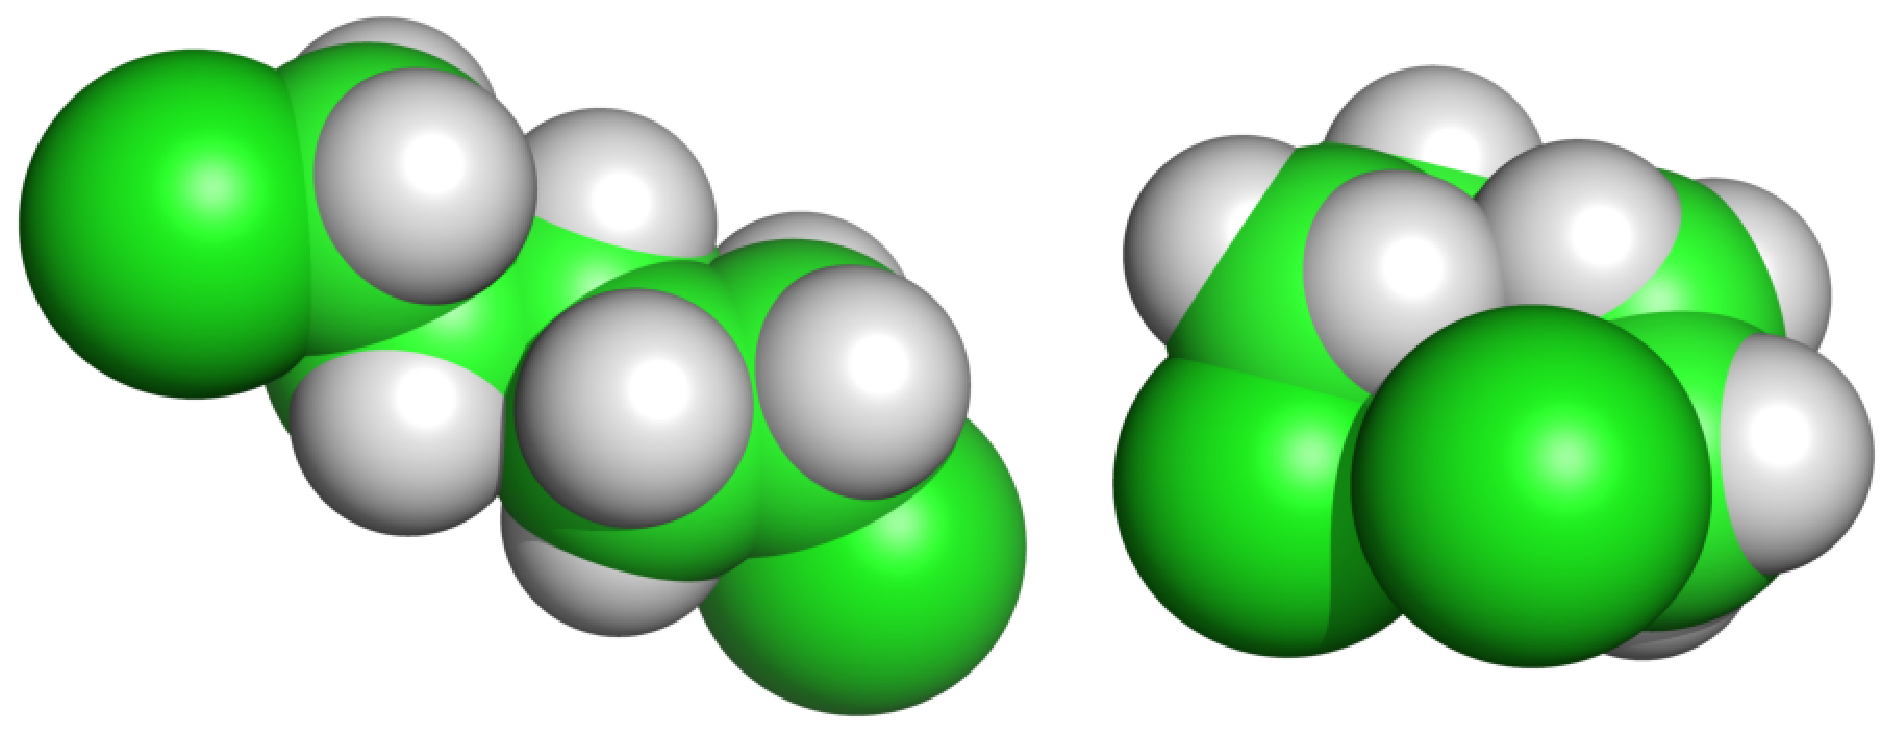
\includegraphics[width=0.25\textwidth]{fig/m040-conformations}
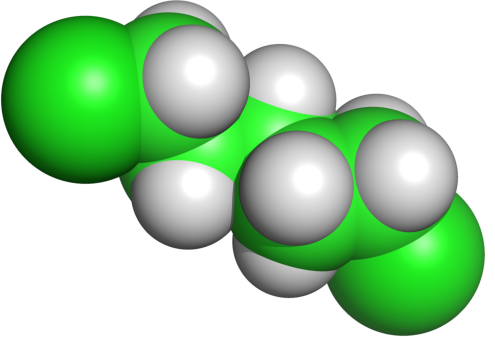
\includegraphics[width=0.14\textwidth]{fig/m040-conf1} \hskip 25pt
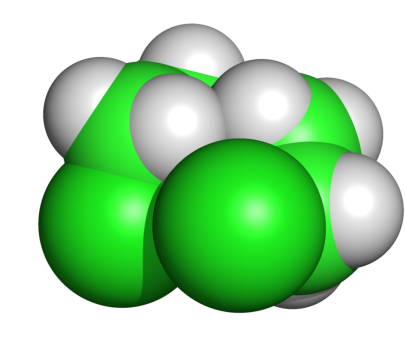
\includegraphics[width=0.11\textwidth]{fig/m040-conf2}
\caption{\label{fig::m040c}
 The examples of a `long' conformation (left) and a `packed' one for the ligand m040 (1,5-Dichloropentane).
}
\end{figure}


%\subsection{Visualization of Results}
%
%TODO Bara: prepsat/motivace/jak se visuazlizuje
%toto je cast textu z toho posledniho paperu. Kdyztak to vyhod.
%
%%In order to fursupport the tunnel exploration process performed by biochemists.
%The above defined characteristics can be shown even as a graph, or better, presented visually by mapping them using colors to the tunnel spheres.
% Alternatively, the surface representation can be used to visualize the tunnel.
%In this case, a 3D point on the tunnel surface is colored according to the property value in its nearest tunnel part $i$,  i.e., such part $i$ whose center $c_i$ is the closest to the point among all tunnel parts.
%
%The examples of the color mapping are shown in Fig.~\ref{fig:properties}.
%The accessibility (Fig.~\ref{fig:properties}a) shows that more than the half of the tunnel is not accessible (red part of the tunnel).
%The throughput shows (Fig.~\ref{fig:properties}b) that the only difficult is the part around the bottleneck (red color in Fig.~\ref{fig:properties}b), and the second half of the tunnel is also traversable.
%
%\begin{figure*}[h]
%\centering
%\begin{tabular}{ccc}
%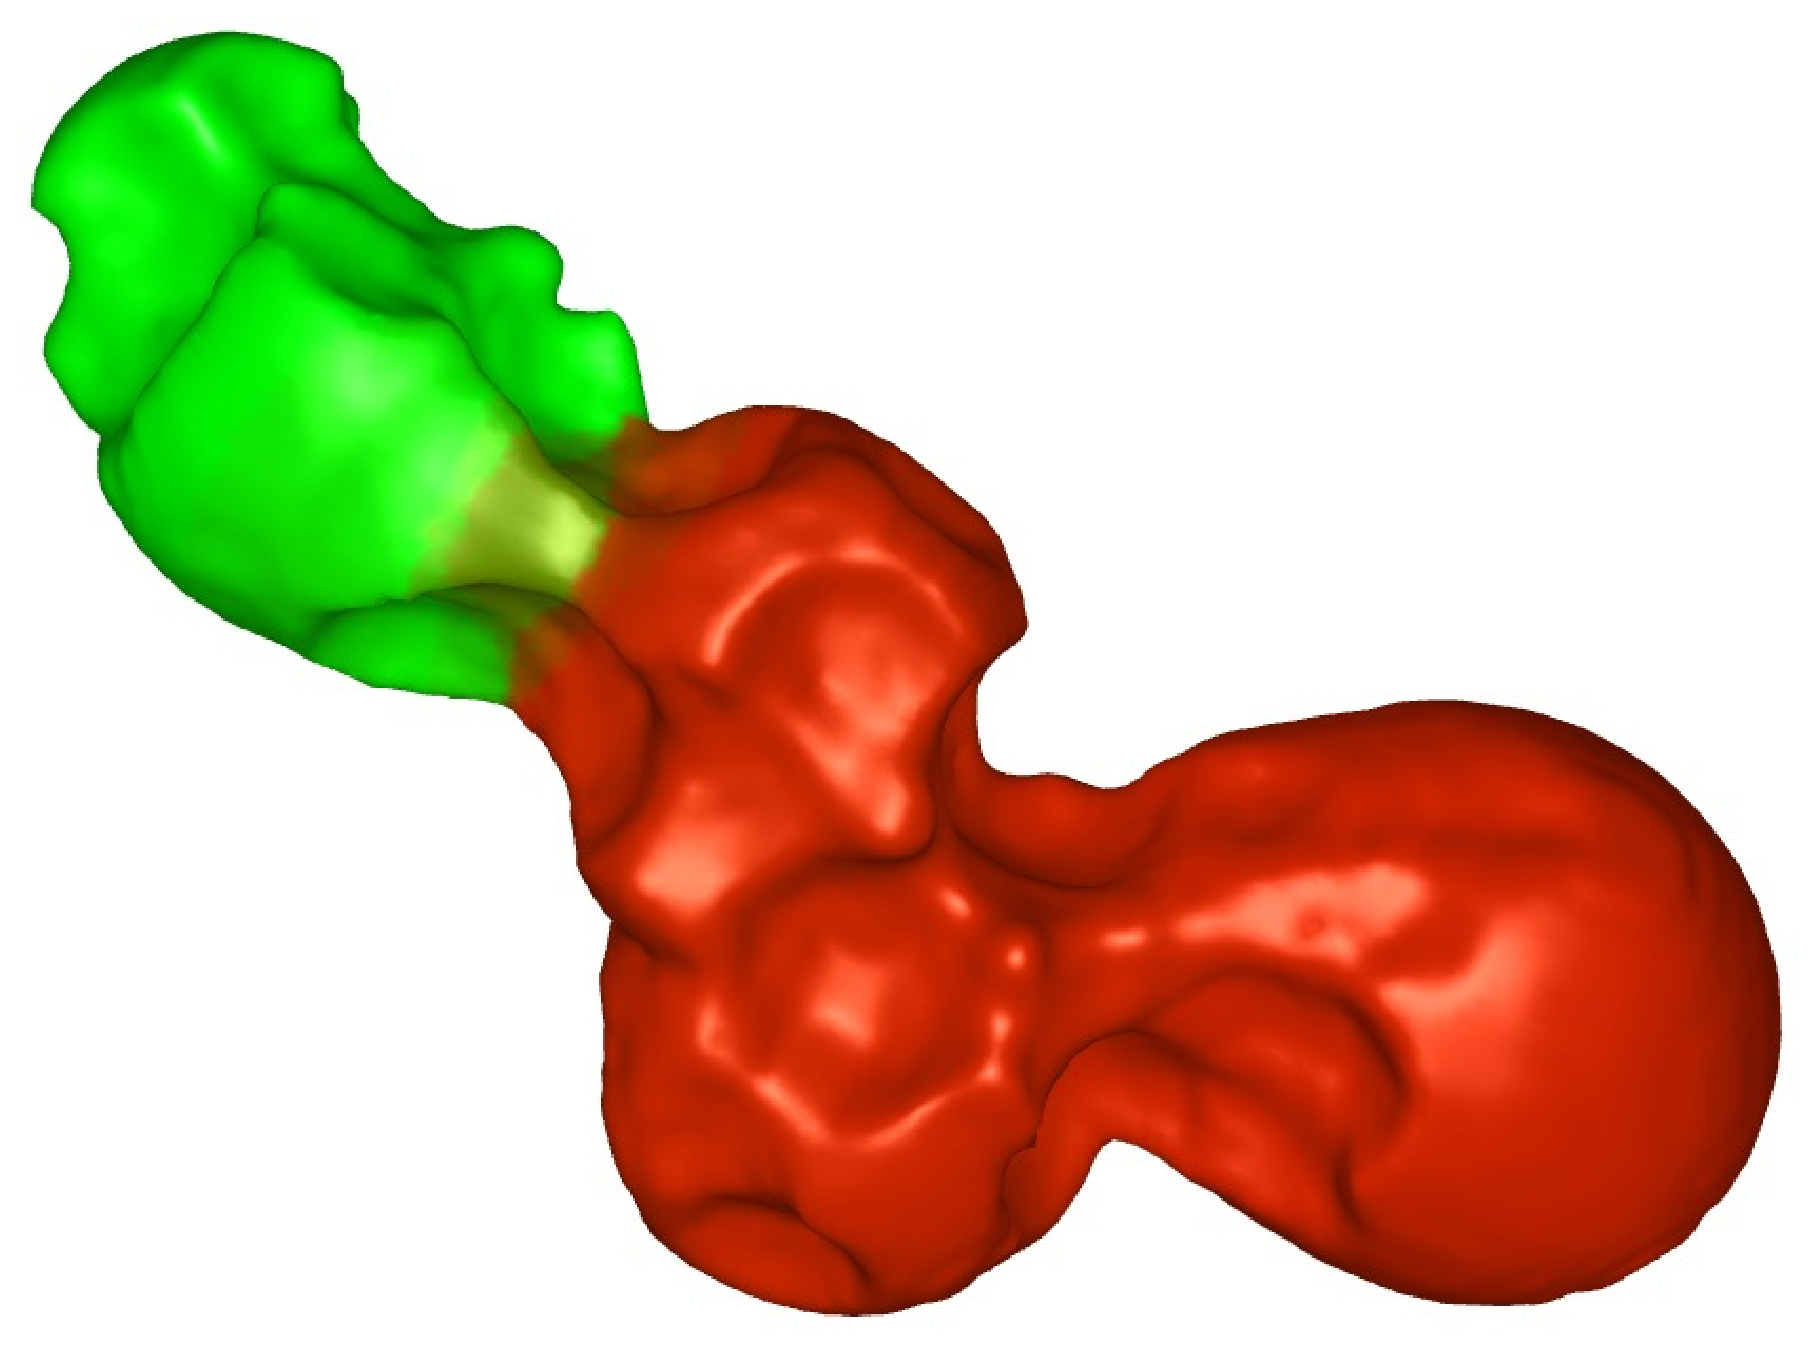
\includegraphics[width=0.3\textwidth]{fig/accessibility} &
%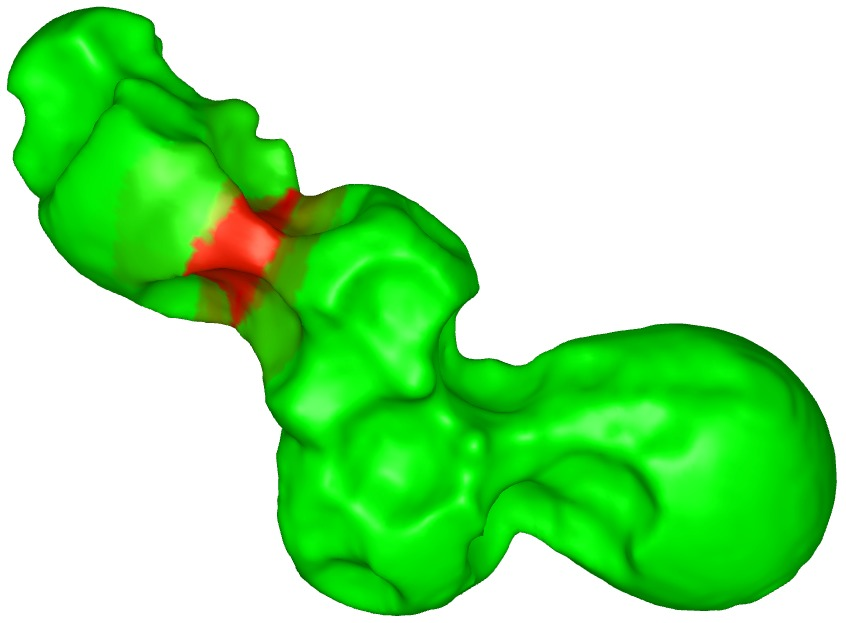
\includegraphics[width=0.3\textwidth]{fig/throughput} &
%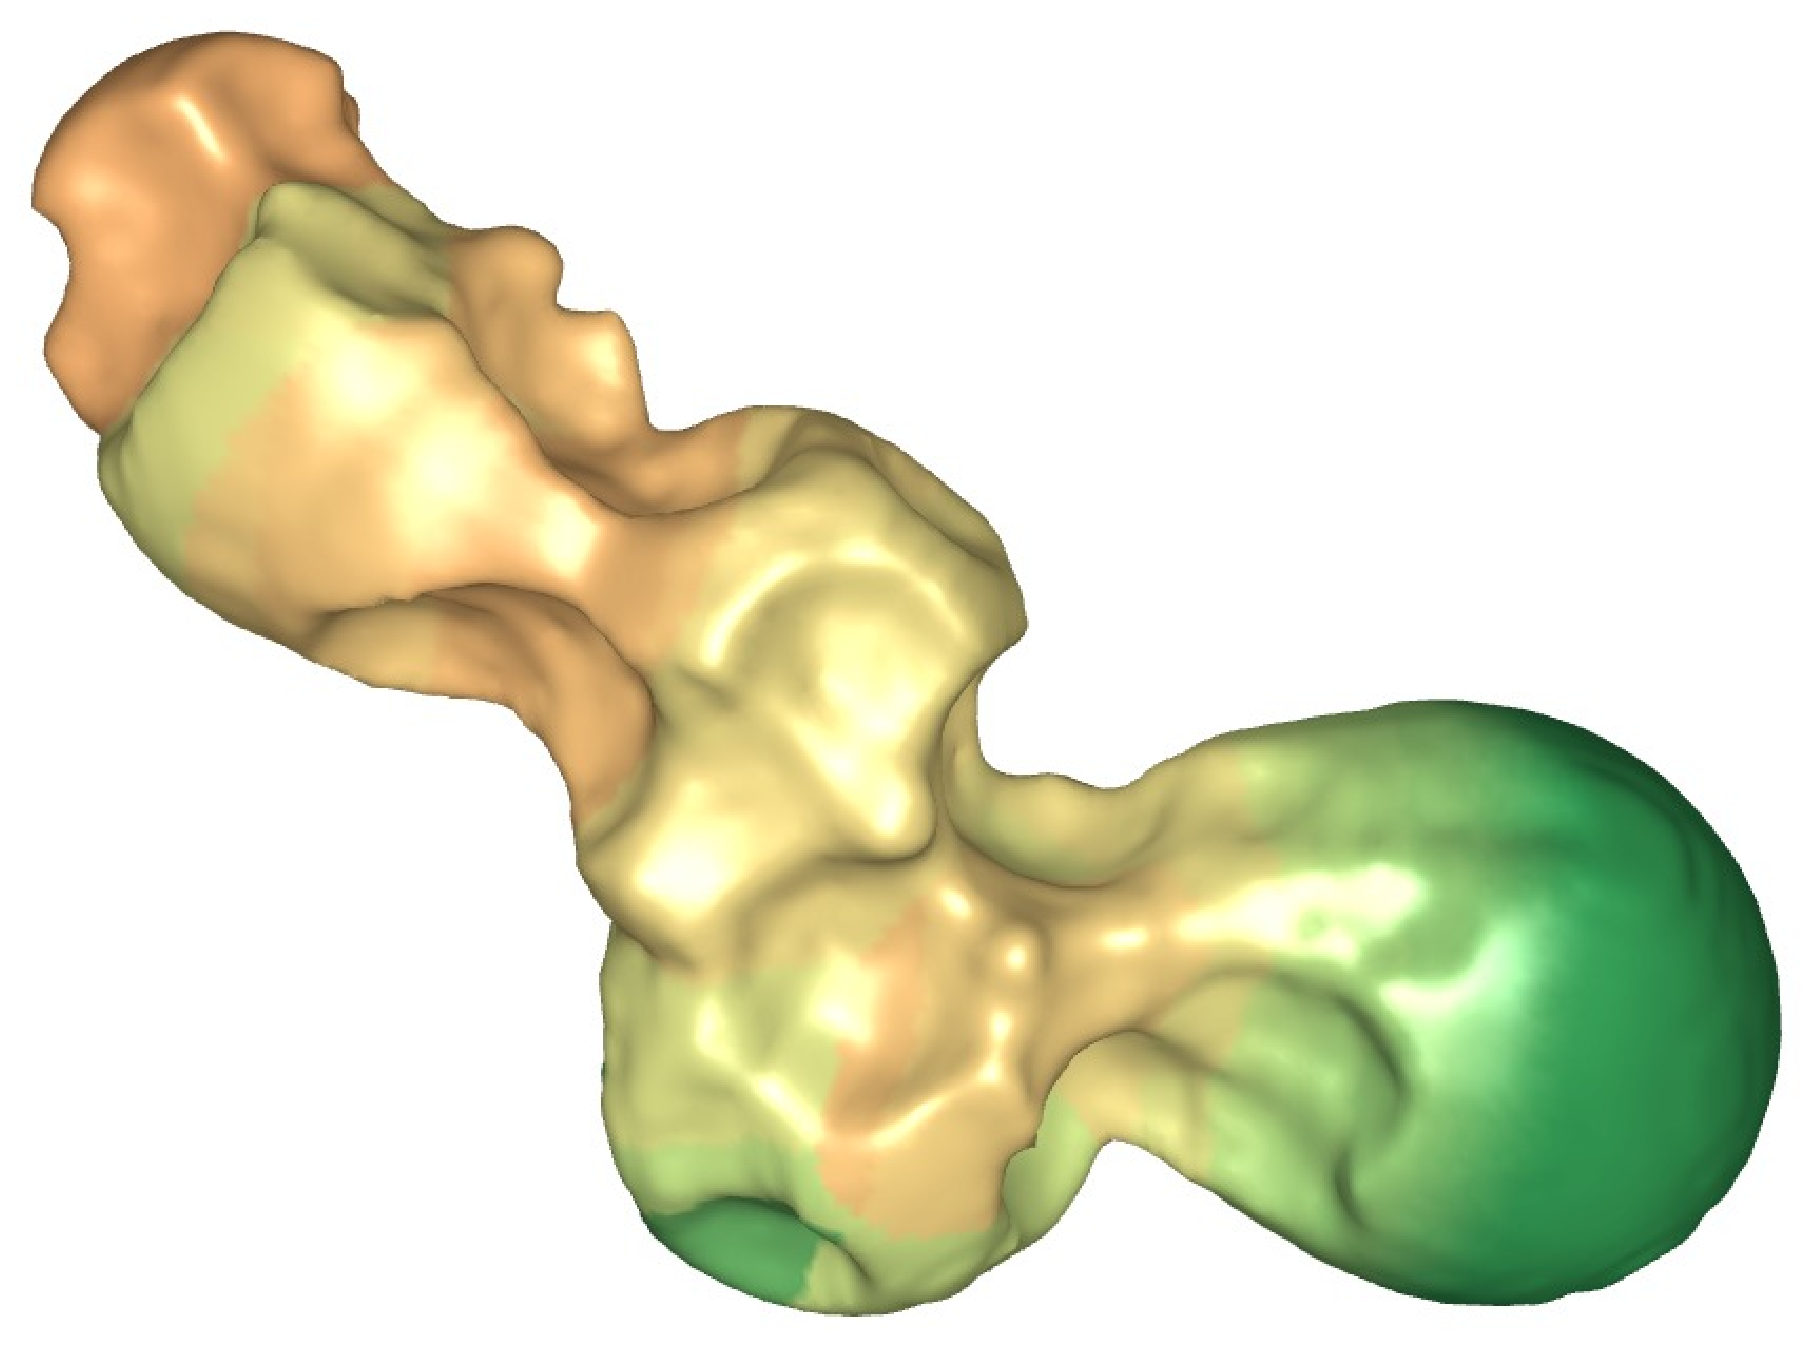
\includegraphics[width=0.3\textwidth]{fig/ligand-scale} \\
%  (a) & (b) & (c) \\                     
%\end{tabular}
%\caption{Tunnel properties mapped onto its surface. The tunnel begins at the top left corner.
%(a) Accessibility --- green denotes the parts that were accessed by the ligand easily ($A(i) > 80$~\%), 
%    while red denotes parts that were accessible  in $<10$~\% of cases.
%(b) Throughput --- green denotes parts that are highly probable to be passed by the ligand ($T(i) > 80$~\%), 
%    while red denotes those that were hard to pass ($T(i) < 20$~\%).
%(c) Ligand scale --- the average scale of the ligand was \tylde 50\% in orange parts, \tylde 60\% in yellow parts, \tylde 80\% in yellow to green parts and \tylde 100\% in green parts.
%\label{fig:properties}
%}
%\end{figure*}
%
%

%\def\cstart{\overline{c_{start}}}
%\def\cend{\overline{c_{end}}}



\section{Experimental Verification}


The proposed approach was used to analyze tunnel traversability towards the active site of Haloalkane dehalogenase protein (PDB ID 1CQW).
The active site was defined using residues 38 (Asparagine), 102 (Histidine) and 103 (Aspartate).
The molecular dynamics of the protein was computed using the Amber tool.
In each frame, tunnels for the spherical probe 0.9~\AA\ were detected using CAVER 3.0~\cite{caver3}. 
In most of the frames, two tunnels were detected.
The average bottleneck of the tunnels are $1.48$~\AA\ and $1.2$~\AA\ for the first and the second tunnel, resp.
The tunnel traversability was analyzed in 100 frames.

Four different scaling-down factors were used: $\S=\{0.5,0.6,0.7,0.8\}$.
For each scale, $|\QI|=20$ collision-free initial configurations were found in the $\RI=2$~\AA\ radius around the first sphere of the tunnel (outside the protein).
For each frame, minimal scale $\smin$ and each initial configuration, 10 trajectories were computed, which resulted
in $100 \times 4 \times 20 \times 10 = 80,000$ trajectories per ligand.

Two motion planners were utilized: the proposed planner (described in Alg.~\ref{alg::main} and Alg.~\ref{alg::expand}), 
    denoted as \RA\ in the rest of the paper, and the Retraction-based RRT~\cite{zhangRetraction} denoted as \RB\ in the rest of the paper.
The \RA\ method was run with the following parameters:
$\Imax=5,000$, $m=100$, $\gb=0.9$, $\dt=1.5$~\AA, $\rv=2$~\AA\ and $\varepsilon=0.05$~\AA.
Both methods were implemented in the same software framework and they utilized the same data structures and routines for collision detection and nearest-neighbor search.
The nearest-neighbor search of both planners is based on the 6D Euclidean metric with the same weights for rotation and translation parts.
This metric was selected based on preliminary experiments with both planners as it resulted in the success rates.

The tested methods differ in the expansion step (lines \ref{alg::expa}--\ref{alg::expb} in Alg.~\ref{alg::expand}).
In these lines, the \RB\ method employs the retraction step in order to find a new collision-free configurations $\qnew$ that approaches $\qrand$.
The retraction step is realized by sampling the vicinity of the configuration $\qnear$ in the distance $0.05$~\AA\ using 20 samples.
A collision-free sample that maximally approaches $\qrand$ is selected and added to the tree, and the retraction continues from this sample.
The retraction step is repeated 5 times.
The \RB\ method can therefore expand the tree by at most 5 new nodes per conformation, while \RA\ extends the tree only by one configuration.
The larger number of nodes in \RB\ method is not problematic, as the KD-trees were used for nearest-neighbor search and the time to solve these queries is significantly less than computing collision detection.
Parameters of the methods were selected in such a way that the number of collision detection queries in each expansion step is same.
For each conformation and tested scale, the \RA\ methods attempts to find $m=100$ collision-free configurations, and \RB\ attempts to perform $5 \times 20$ collision-detection queries.
Other parameters of the \RB\ planner were same as for \RA.
Planning was terminated after $\Imax$ iterations, or if the tree approached the active site to the distance less than 0.5~\AA.

In the following experiments, we measure performance of the methods using the traversability rate, which is the percentage of frames of the protein dynamic that are traversable by the tested ligand.
A frame is considered traversable, if at least one trajectory out of 20 (the number of initial configurations $|\QI|$) $\times$ 10 trials approaches the active site to the distance less than 2~\AA.~\footnote{We refer to~\url{http://mrs.felk.cvut.cz/icra2018protein} for additional material}

\subsection{Traversability of one atom}

The aim of the first experiment is to measure performance of both planner in the simplest scenario: finding path for one sphere towards the active site.
The radius of the sphere is $1.7$~\AA. 

The computed traversability rates are shown in Tab.~\ref{tab::one}.
The maximum percentage of traversable frames (the row Maximum in Tab.~\ref{tab::one}) is computed as the percentage of tunnels with bottleneck larger than the tested radius.
The row Planning shows the traversable rate computed by the planners.
This rate decreases with the increasing radius and it is lower than the maximum traversable rate.
The rates provided by \RA\ and \RB\ are similar which is a good indicator that the methods have been programmed correctly.
Higher traversability rate can be achieved by increasing the maximum number of planning iterations $\Imax$, which would also
increase the planning time.
For the purpose of the following experiments, we used $\Imax=5,000$ as a compromise between the performance and the runtime.

\begin{table}
\centering
\caption{\label{tab::one}Traversability for one atom.}
\renewcommand{\tabcolsep}{4.3pt}
{\small
\input graphProbe.tex
}
\end{table}


%
%{\def\a{270}
%\begin{figure}
%\centering
%\renewcommand{\tabcolsep}{0pt}
%\begin{tabular}{cccc}
%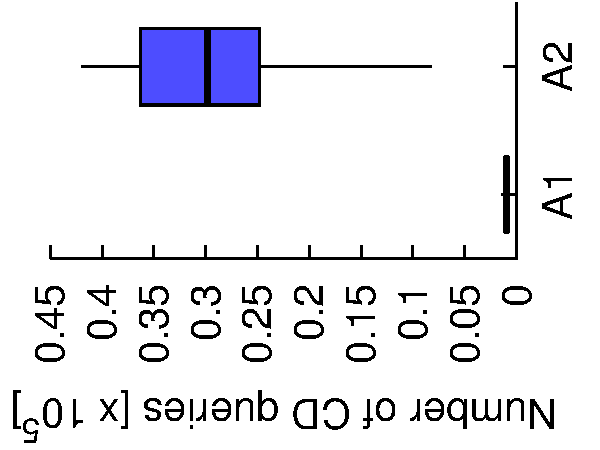
\includegraphics[width=0.15\textwidth,angle=\a]{fig/m001-oneAtom-cdCount} &
%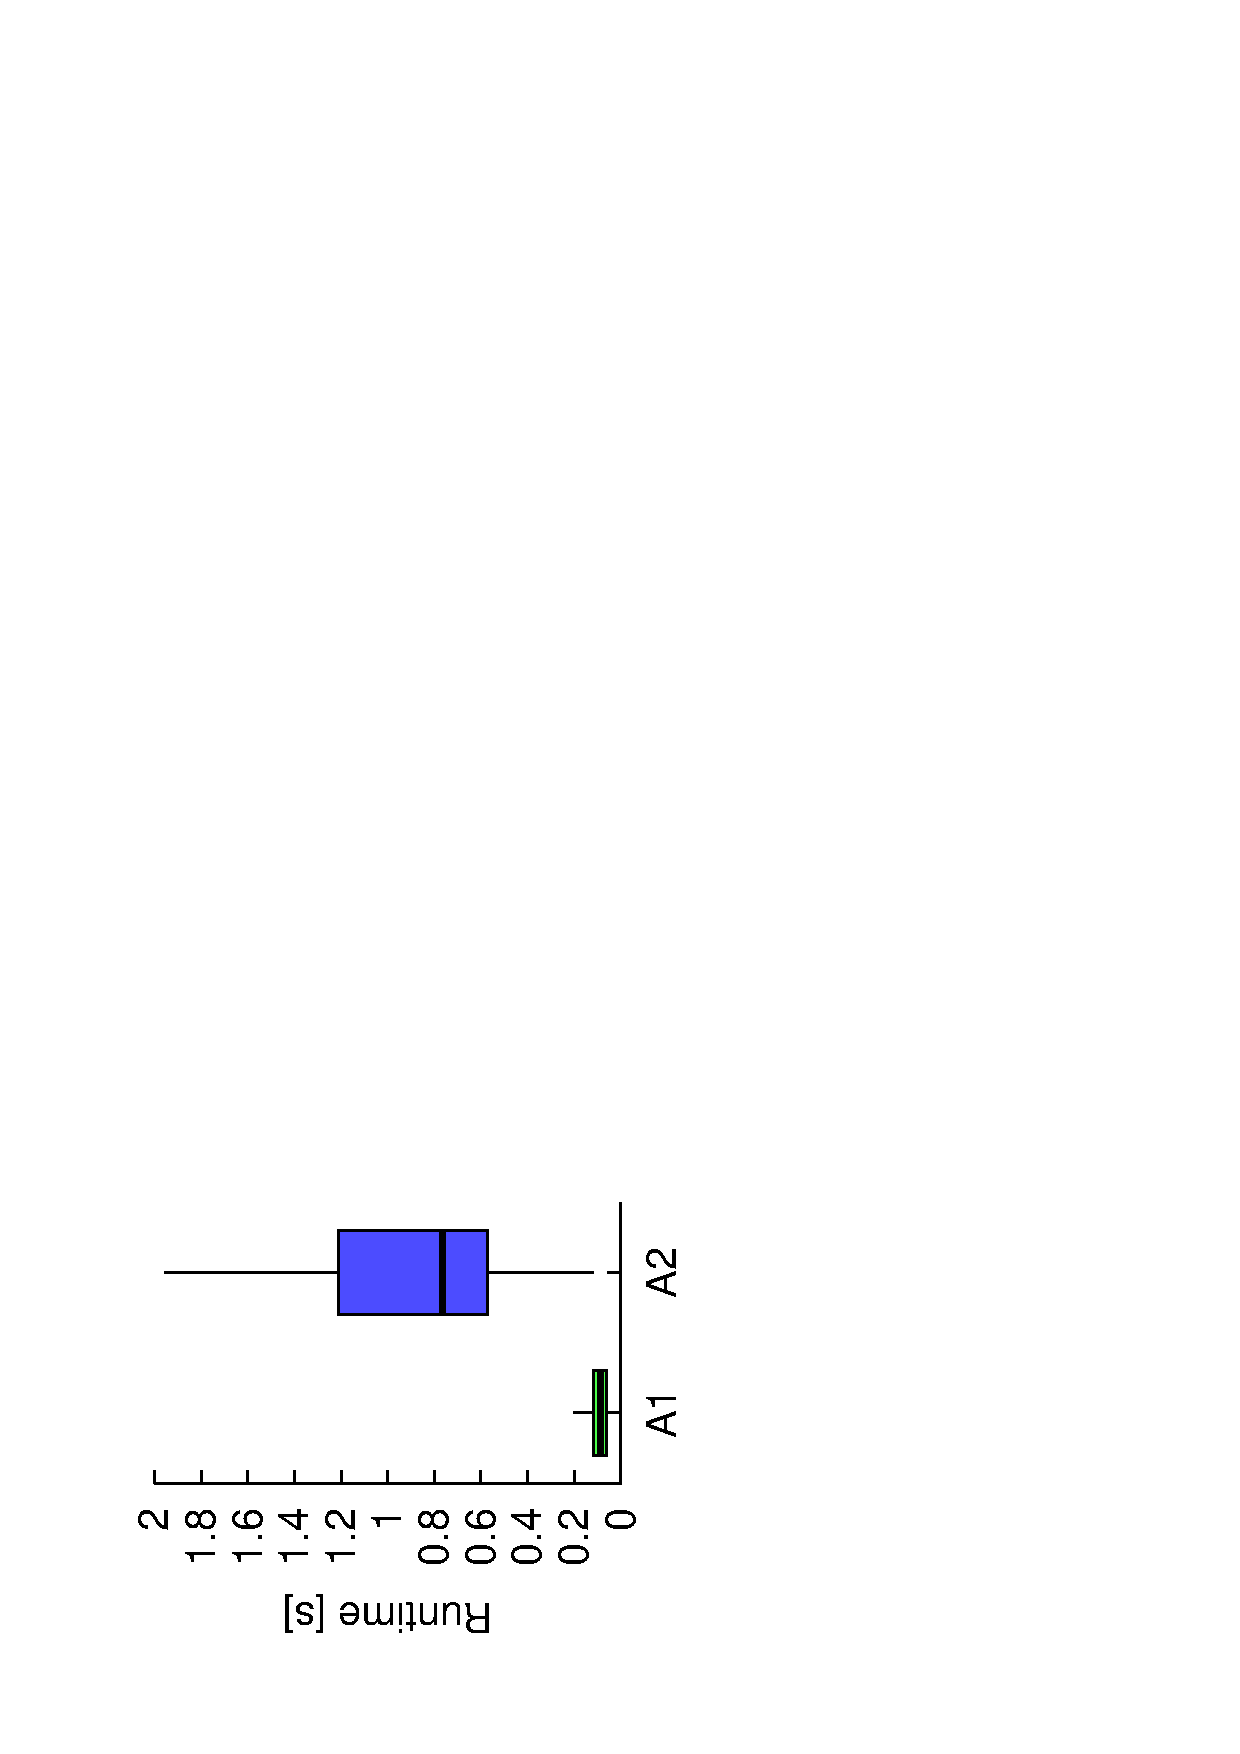
\includegraphics[width=0.15\textwidth,angle=\a]{fig/m001-oneAtom-rrt_path_time} &
%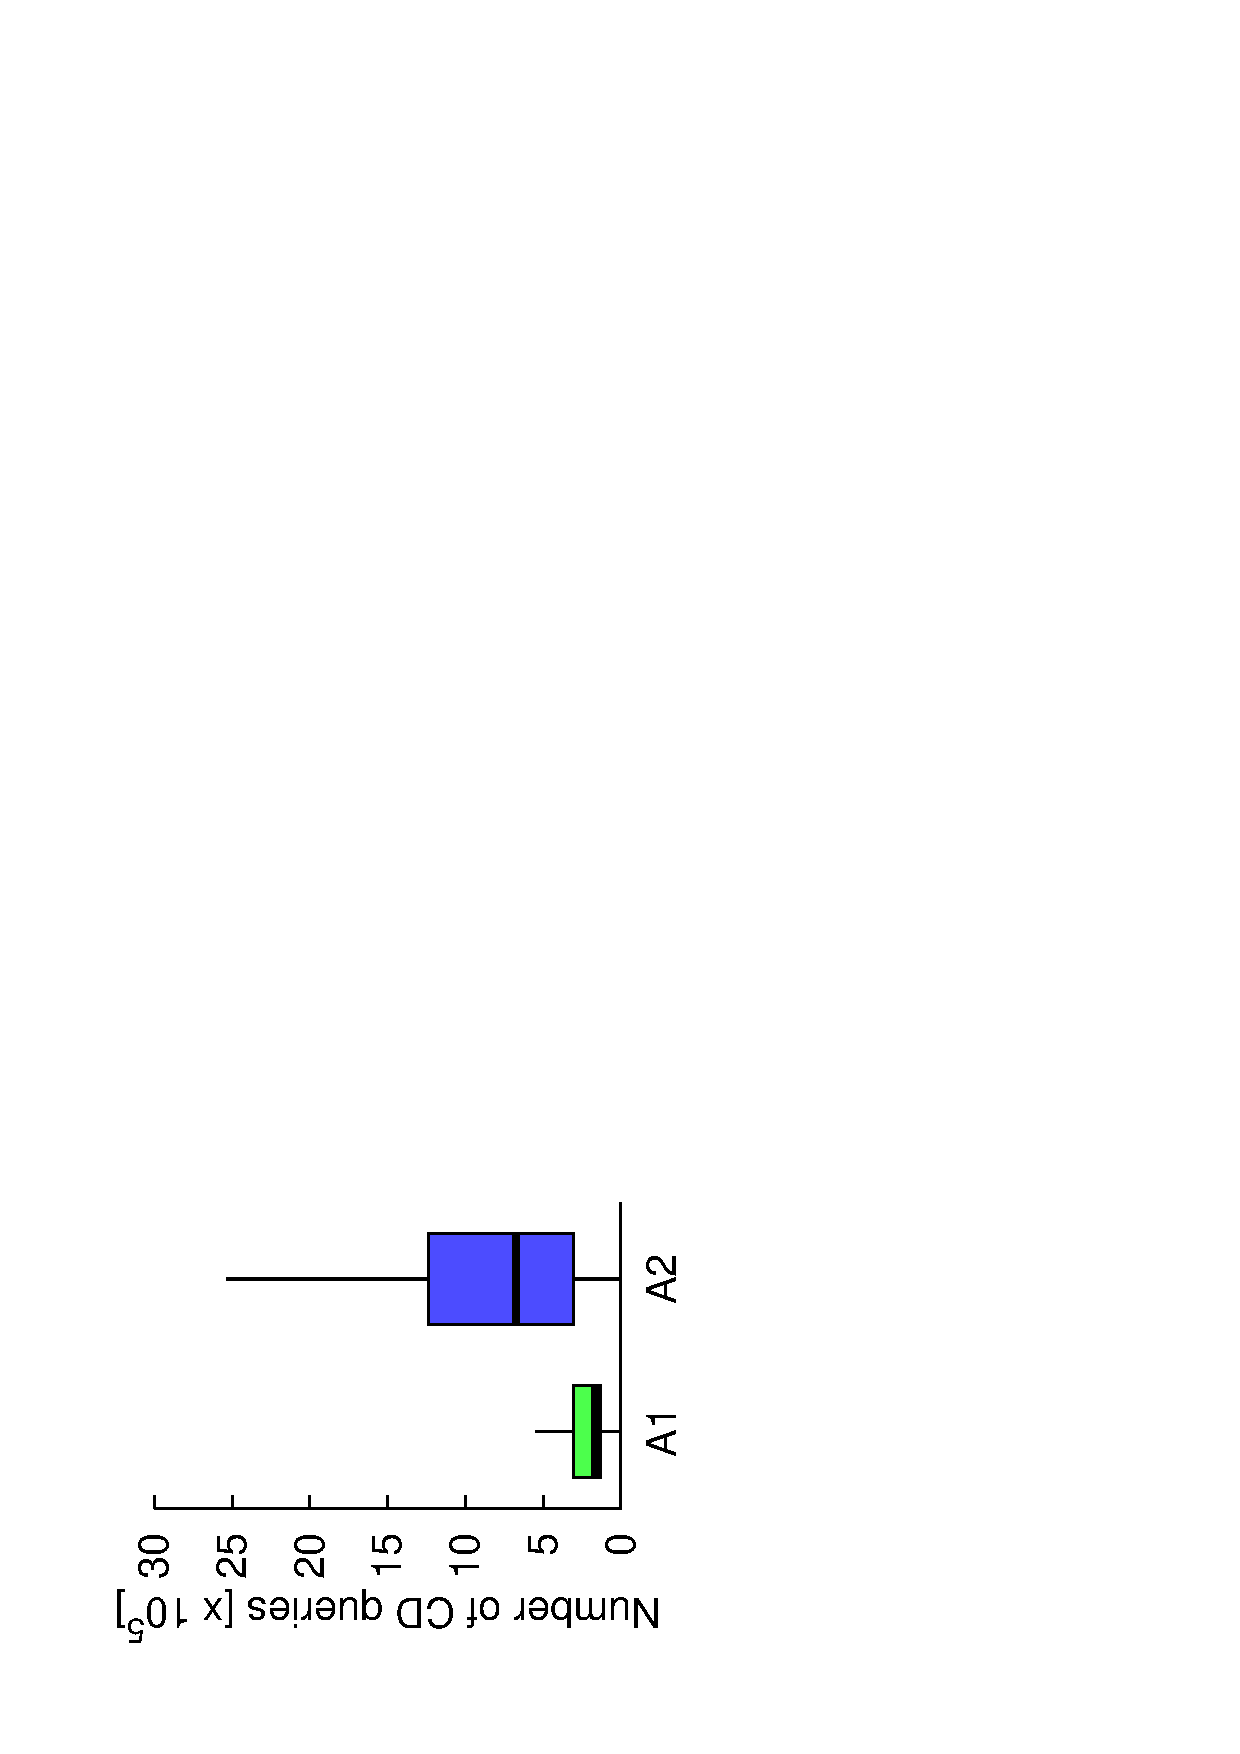
\includegraphics[width=0.15\textwidth,angle=\a]{fig/m037t-cdCount} & 
%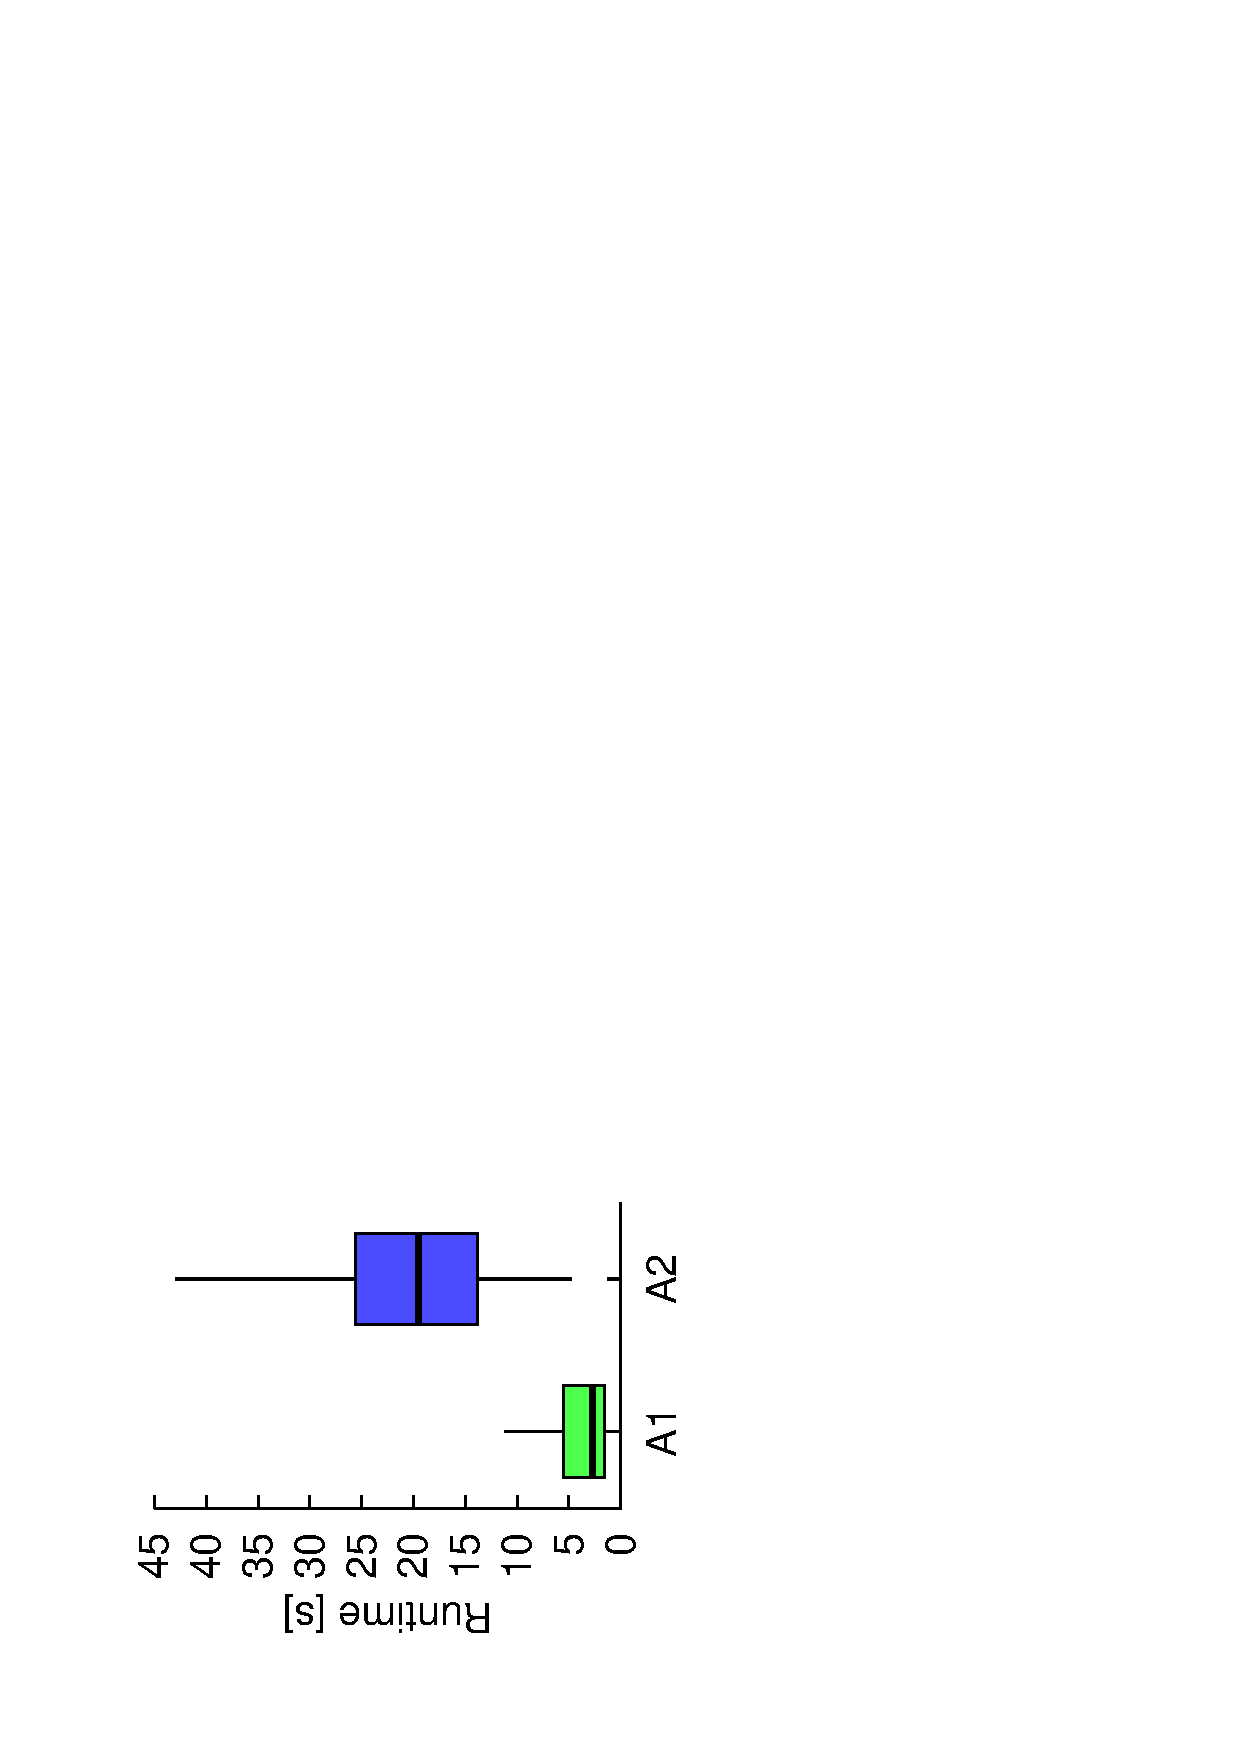
\includegraphics[width=0.15\textwidth,angle=\a]{fig/m037t-rrt_path_time} \\
%\multicolumn{2}{c}{One-atom} &
%\multicolumn{2}{c}{m037}  \\
%\multicolumn{4}{c}{%
%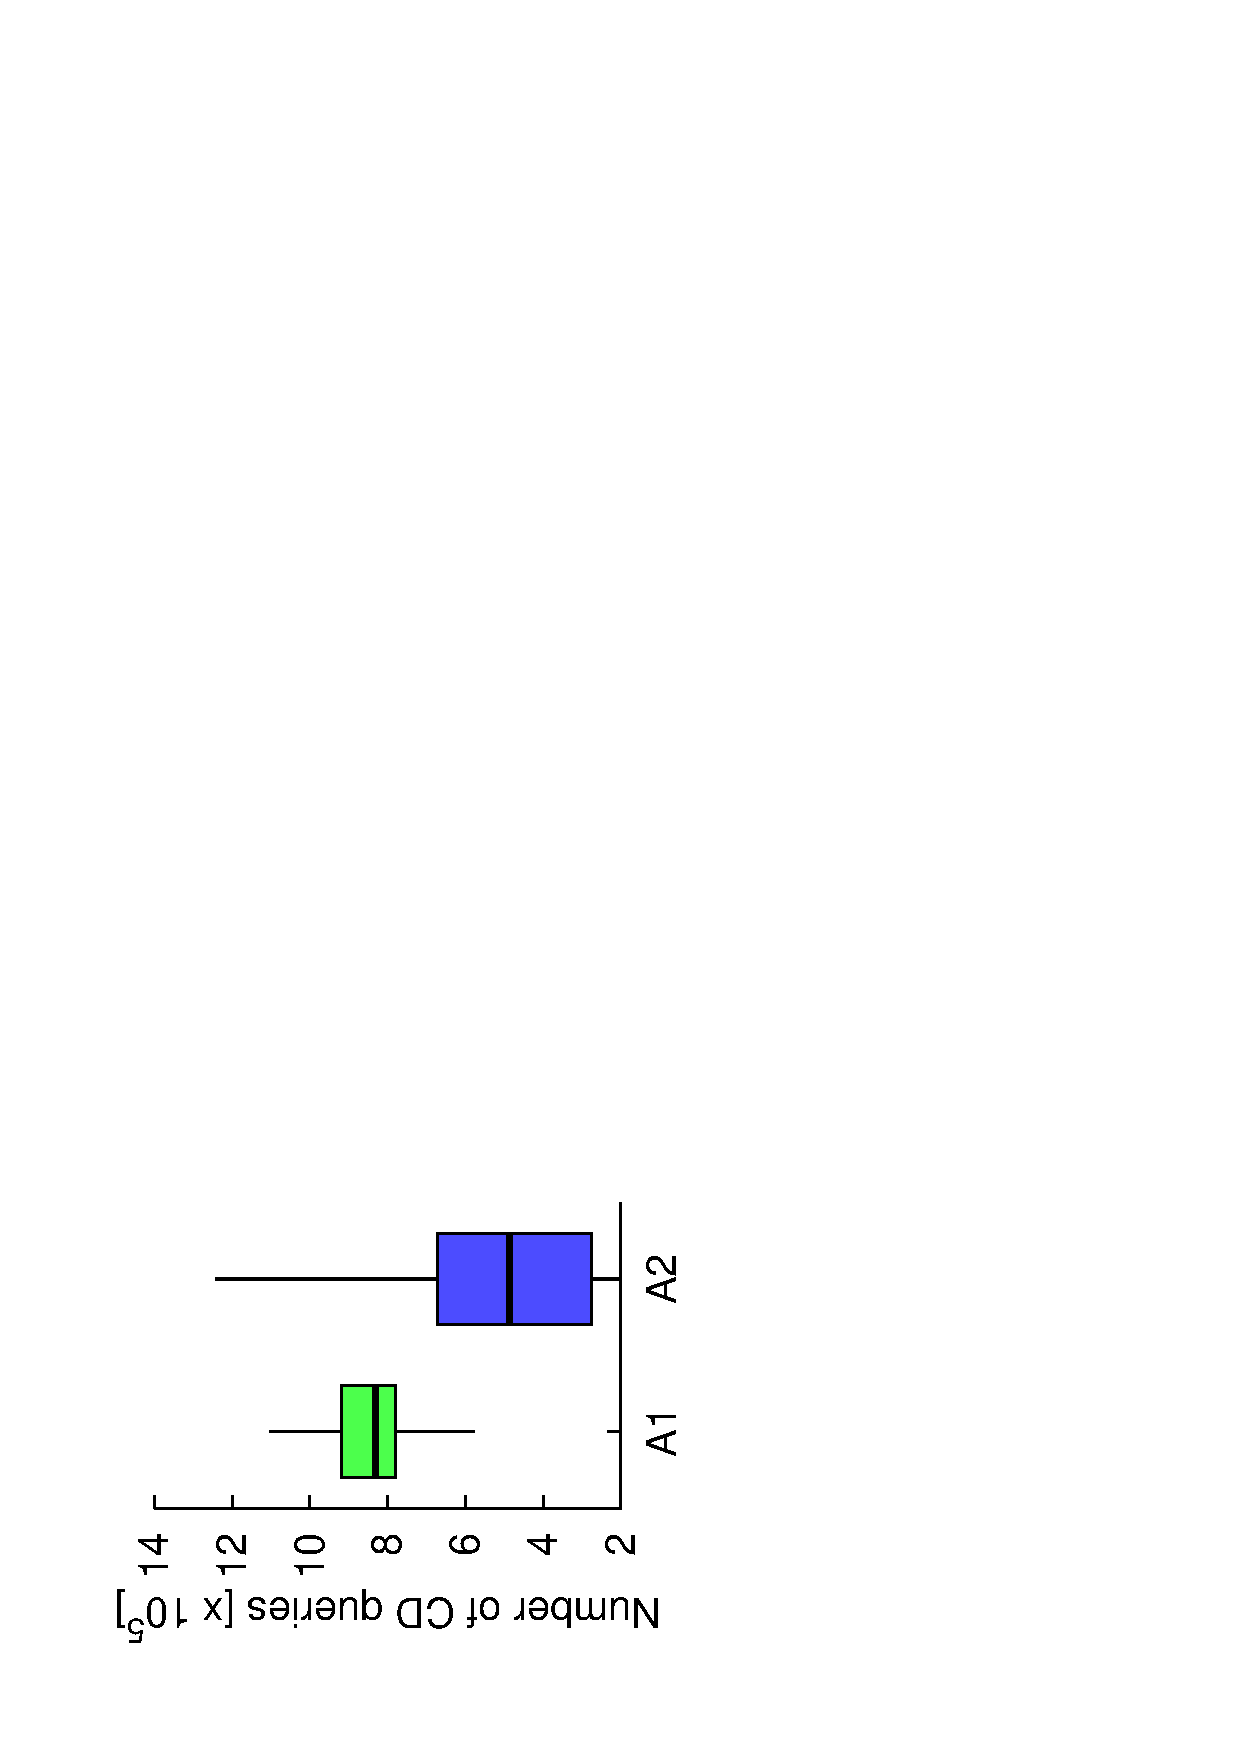
\includegraphics[width=0.15\textwidth,angle=\a]{fig/m040-10-cdCount} 
%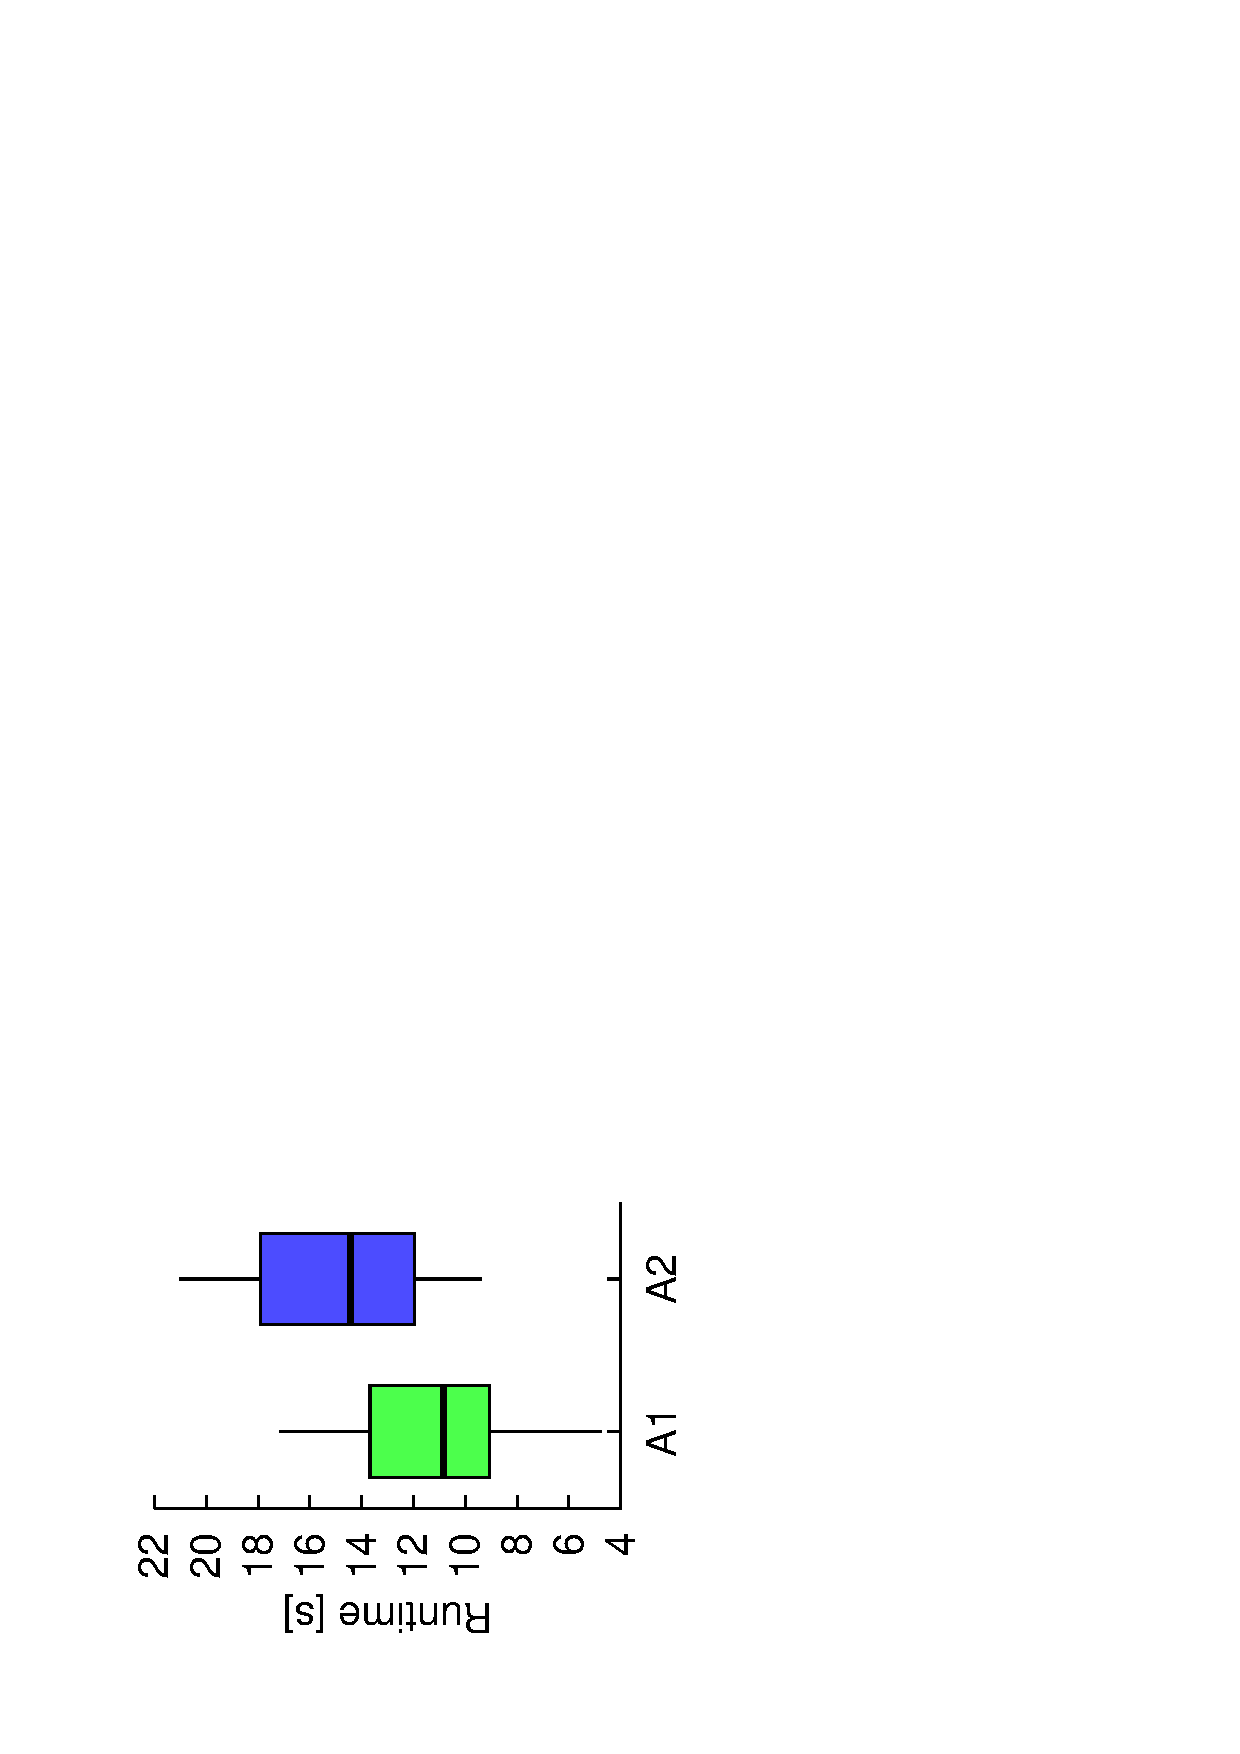
\includegraphics[width=0.15\textwidth,angle=\a]{fig/m040-10-rrt_path_time} 
%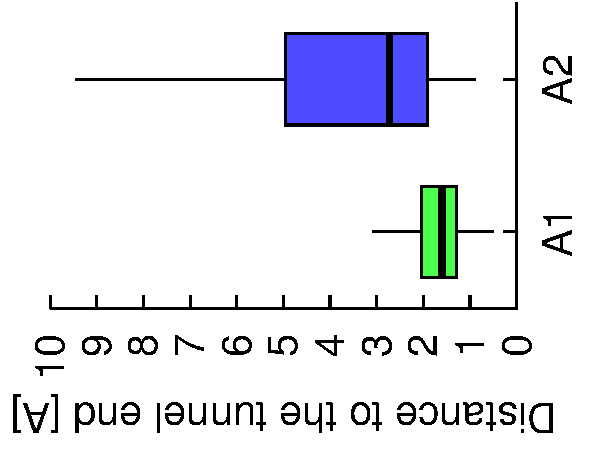
\includegraphics[width=0.15\textwidth,angle=\a]{fig/m040-10-trajDistToGoal}} \\
%\multicolumn{4}{c}{m040} 
%\end{tabular}
%\end{figure}
%}
%





%\begin{figure}
%\centering
%\begin{tabular}{cc}
%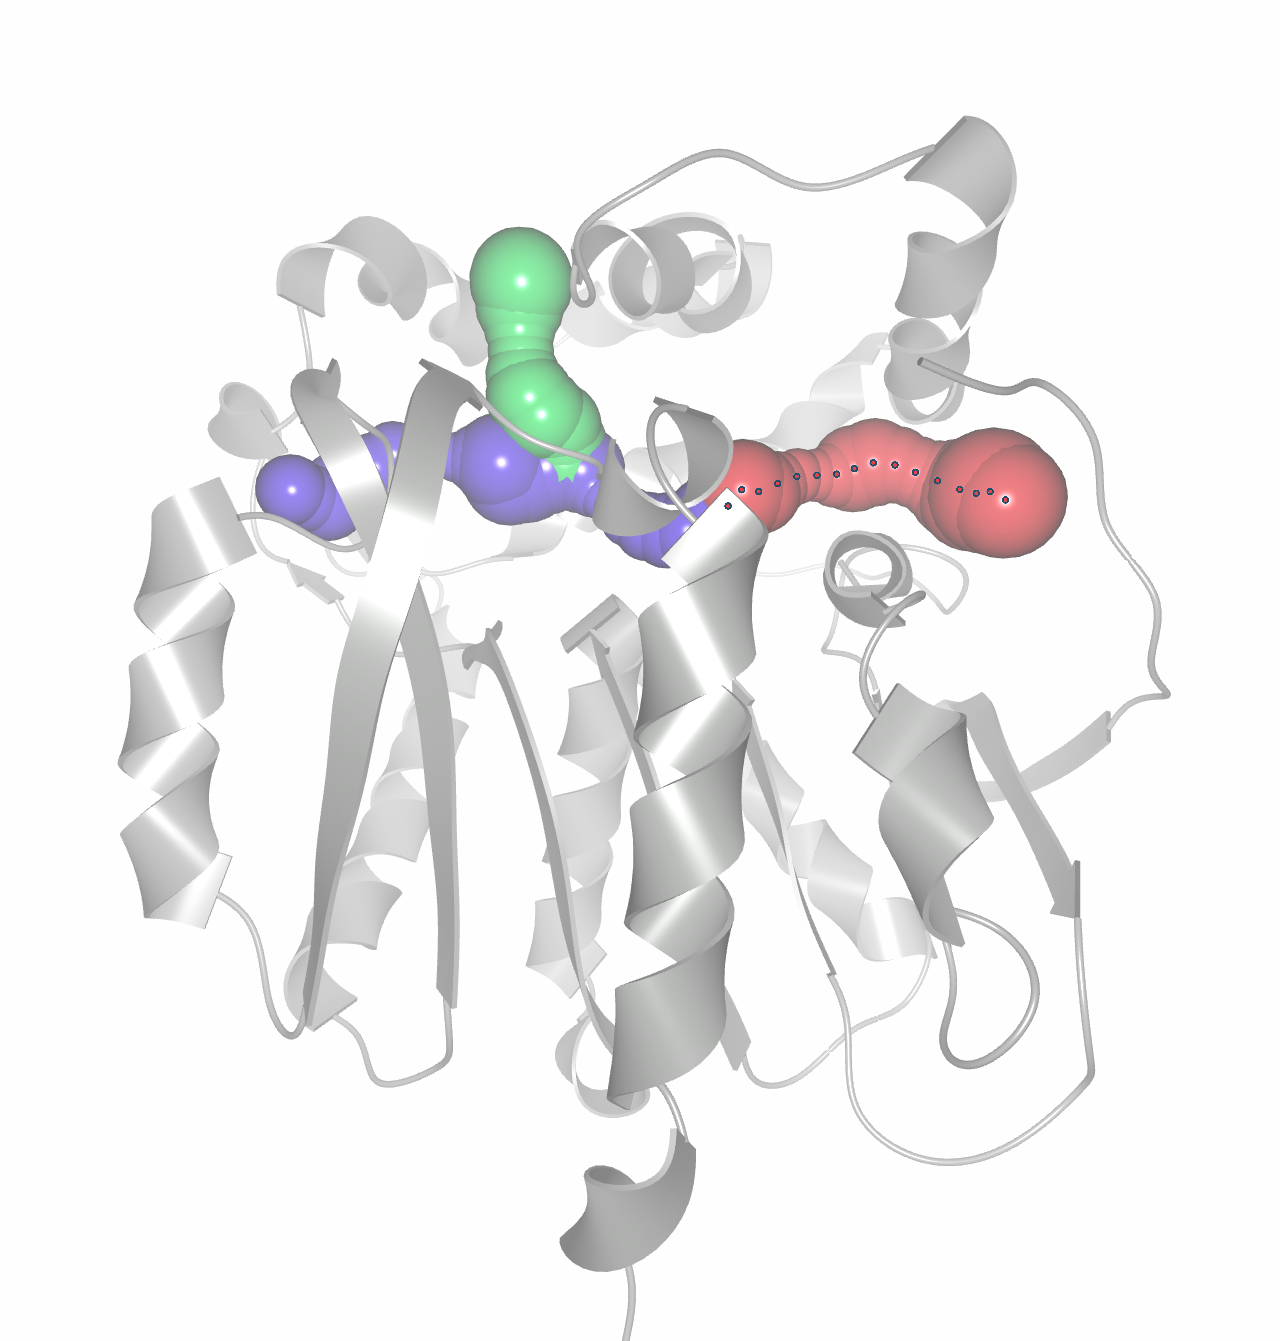
\includegraphics[width=0.3\textwidth]{fig/t05proteintunnels} &
%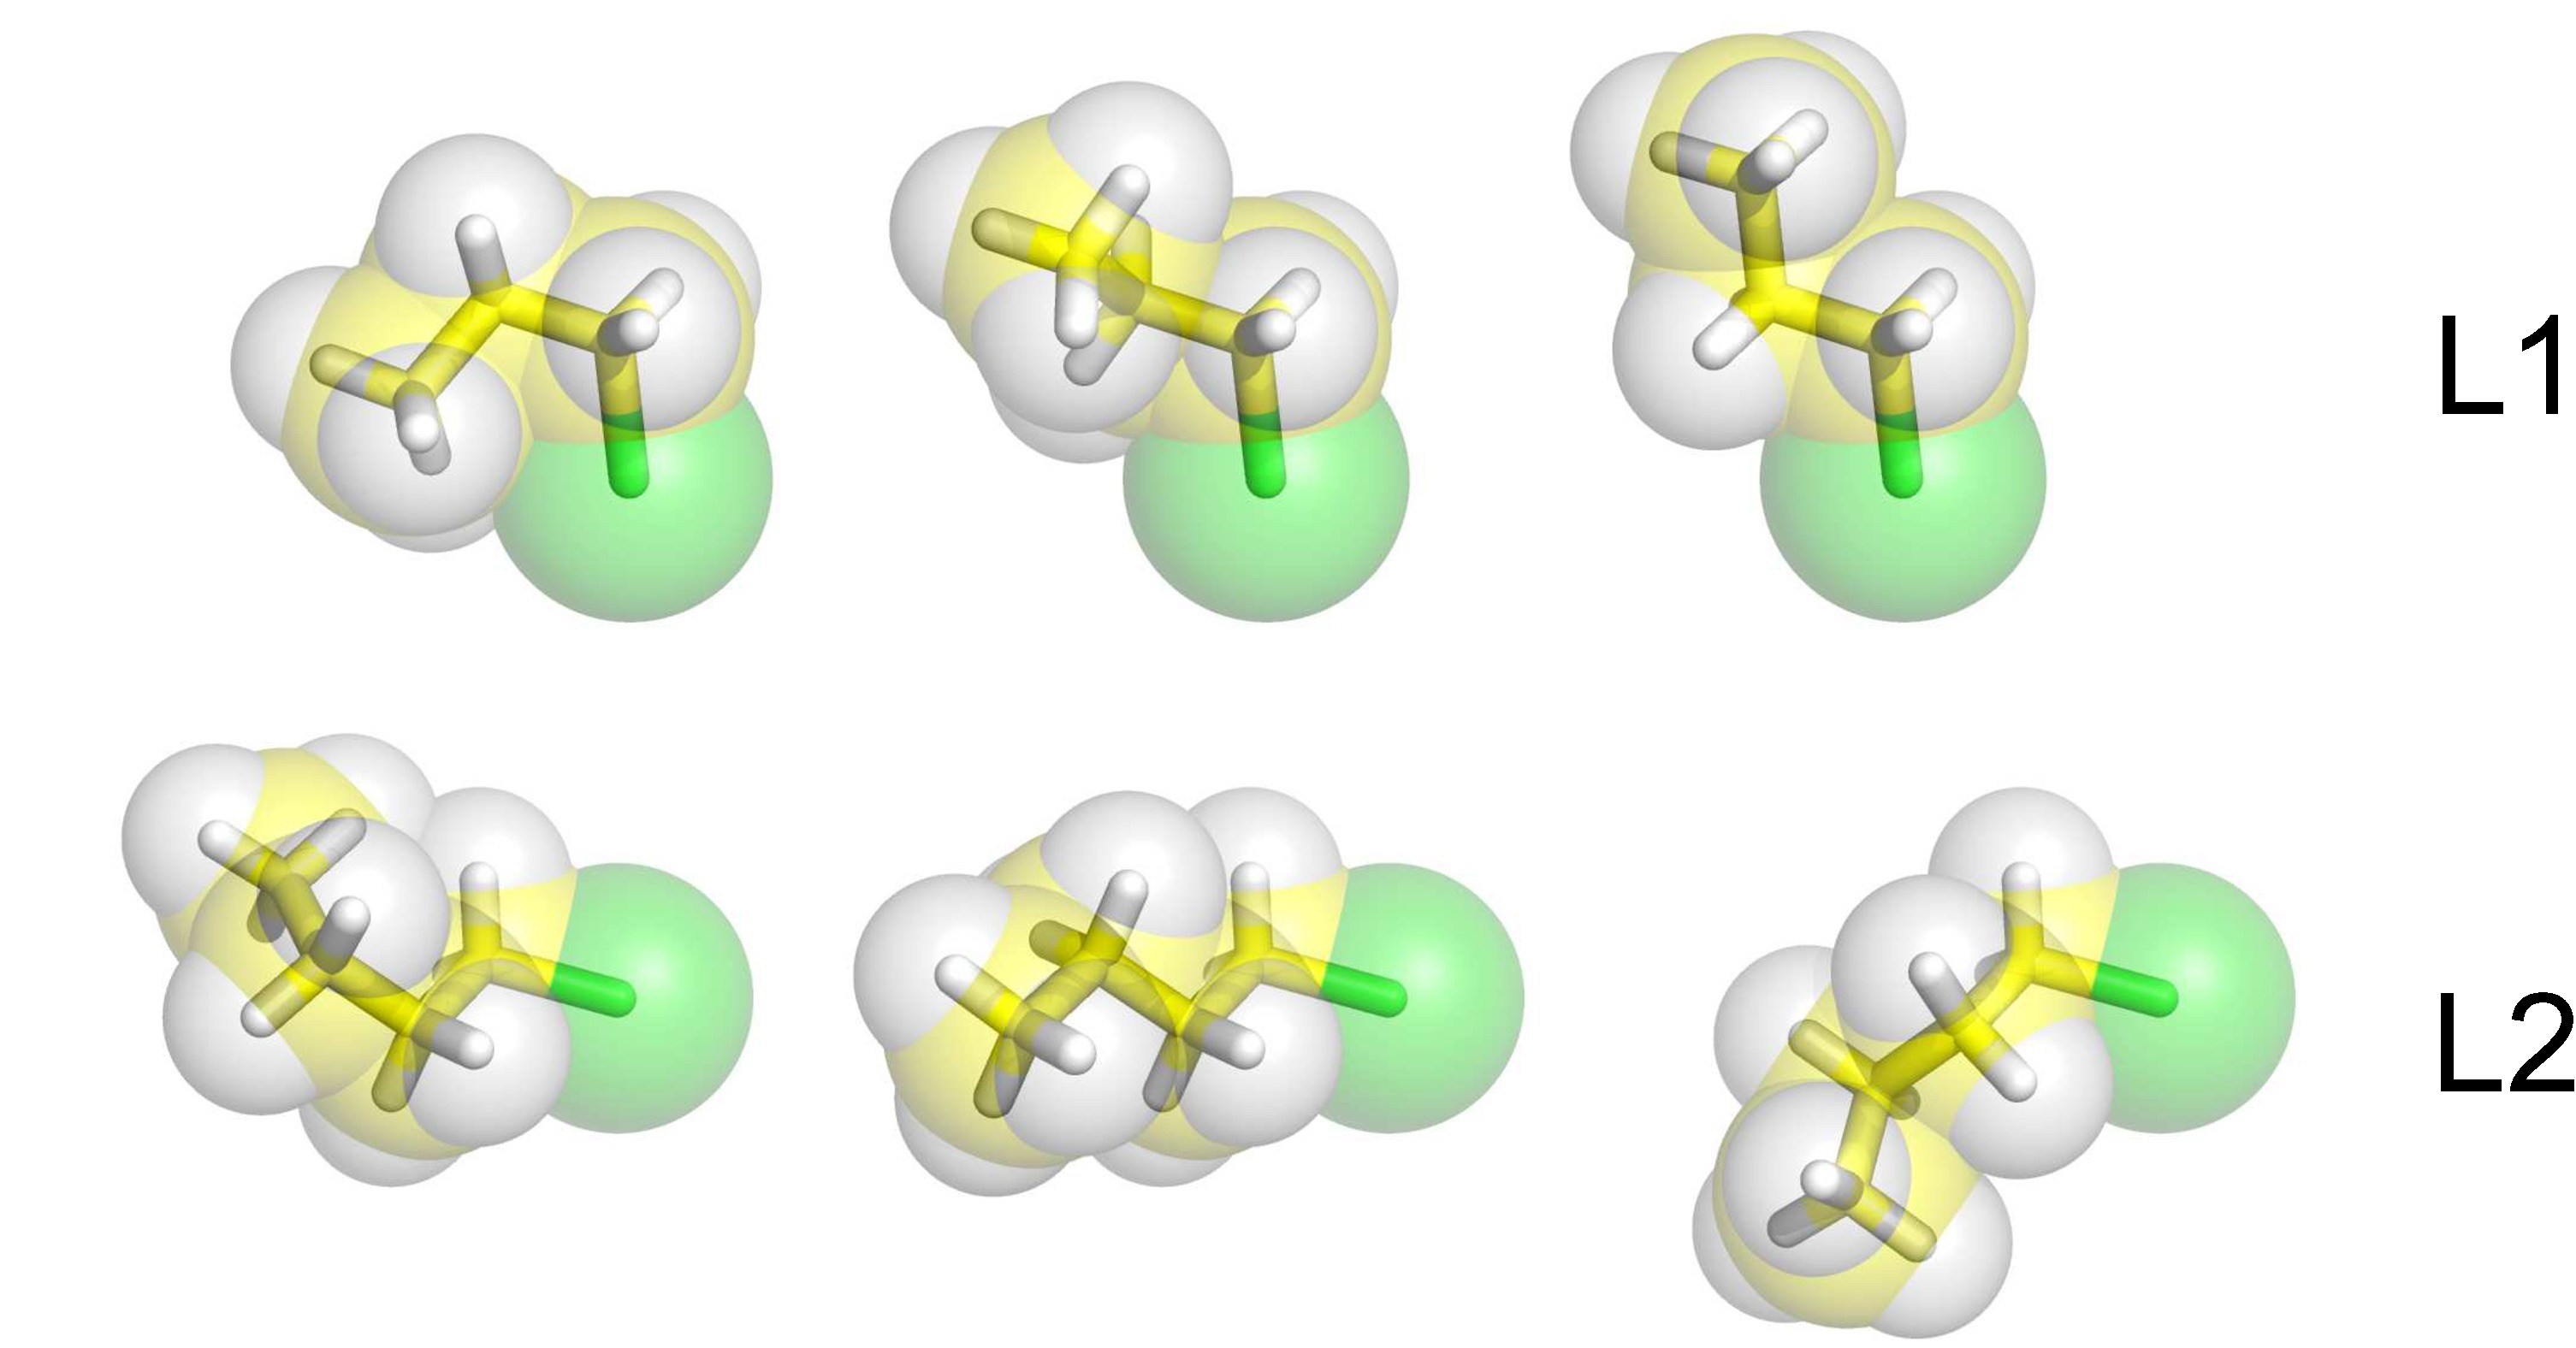
\includegraphics[width=0.45\textwidth]{fig/ligAll}  \\
%(a) & (b)                        
%\end{tabular}                       
%\caption{\label{fig::tunnel}
%    (a) The protein 1CQW visualized using the cartoon representation (gray) with 
%        three tunnels (red, green, blue) detected by CAVER 3.0.
%        The first tunnel is depicted red.
%%        its highest ranked tunnel (green) which was detected using CAVER 3.0.
%    (b) Examples of three conformations of $\LA$ (top) and $\LB$ (bottom)
%}
%\end{figure}
%

\subsection{Influence of the conformation selection}

The aim of this experiment is to verify the procedure to select ligand conformations for the motion planning.
The experiment was performed with the ligand DCP (Dichloropropanol), for which $1300$ conformations where available and for the ligand
m040 (1,5-Dichloropentane) with $7560$ available conformations.
Two strategies were tested: the strategy described in Sec.~\ref{sec::strat} (denoted `S') and a strategy that prefers smaller conformations (denoted `P').
The `P' method selects such conformations where the deviation of the atomic distance from the geometric center are lowest, which leads 
to selection of the packed conformations (Fig.~\ref{fig::m040c}).

The traversability rates are shown in Tab.~\ref{tab::selection}, where the subscript of each ligand's 
name shows the number of the selected conformations (5 or 50) and the used method (S or P).
The number after the slash in the ligand's name denotes the number of atoms of the ligand.
In the case of both tested ligands and 50 selected conformations, the `S' strategy leads to higher traversability rate than the `P' strategy.
For the ligand DCP, a higher traversability rate was achieved when 50 conformations were selected.
This experiments shows that selecting 50 conformations using the `S' strategy (Sec.~\ref{sec::strat}) leads to better results
than using less number of conformations or when preferring the packed conformations.

\begin{table}
\centering
\caption{\label{tab::selection}
    Influence of the conformation selection method to the traversability rates in the first tunnel.
    The number after~`$/$' denotes the number of atoms.
}
\small
\renewcommand{\tabcolsep}{4.3pt}
{\small
\input graphSel.tex
}
\end{table}





\subsection{Traversability of ligands}

Based on the results of the previous experiment, 50 conformations using the `S' strategy were selected for the following
ligands: m037t (1,2-Dichloroethane), m038t (1,3-Dichloropropane), m056 (2-Chlorobutane) and m080 (Trichloropropane), and
the task was to compute trajectories for these ligands in the MD sequence.

The results are summarized in Tab.~\ref{tab::main}.
The table shows the traversability rate only for the first tunnel, as no trajectory was found in the second tunnel for most of the tested ligands.
The only exception is the ligand m037t, which was the smallest tested ligand (with 8 atoms), and therefore it can fit even inside the second tunnel.
The traversability rate is higher for the most scaled-down ligands ($\smin=0.5$) and it decreases with the increasing scale.
For the scale $\smin=0.8$, the most traversable frames were detected for ligands DCP (8~\%), m037t (20~\%) and m038t (16~\%).

{\bf doufam, ze toto neni moc drze:}
The traversability of the DCP ligand to active site was approved by the MD simulation.
The observed trajectory of the DCP ligand in the MD simulation followed the first tunnel.
Based on the traversability rates with $\smin=0.8$, we expect that at least ligands m037t and m038t can also reach the active site, as
they have same (or even larger) traversability rate than DCP.
However, this hypothesis hasn't been tested against MD simulations yet.

The proposed \RA\ planner provides higher traversability rate than \RB.
The distances of the configuration trees (measured using 3D Euclidean metric) to the active site and the runtimes in each frame
are shown in Fig.~\ref{fig::comparison}.
The runtimes of both algorithms increase in those frames, where the tunnel is not traversable, i.e., where the distance
to the active site is more than 2~\AA\ (for example,in the frame number 60).



The most time consuming part of the planners is the collision detection. 
Although the both methods can utilize the same number of collision detection queries in the expansion step, \RB\ is slower than \RA.
The reason is, that \RA\ expands the tree more closer to the random samples $\qrand$ than \RB.
This results in a faster exploration of the configuration space and therefore, \RA\ needs less number of iterations to reach the active site.
The better performance of \RA\ is caused by the proposed atom-based metric, because this distance depends on the actual shape of the ligand and 
it allows the ligands to retract more toward $\qrand$.
Contrary, \RB\ utilizes the single 6D Euclidean weighted metric in the expansion, where the weights are same for all conformations.
Depending on these weights, the metric favors samples that differ from $\qrand$ more in rotation or translation part.
However, the weights between rotation/translation parts should depends on the shape of the ligand, which is different in each conformation.
By using single set of weights in the 6D Euclidean metric, we implicitely favor either the packed or the longer conformations.
%To improve performance of \RB, the weights of the 6D Euclidean metric should differ for each conformation, but it would
%prevent the usage KD-tree for the nearest-neighbor search.

\begin{table}
\centering
\caption{\label{tab::main}
    Traversability of the tunnels for ligands with 50 conformations. 
    The number after '$/$' denotes the number of atoms.
}
\small
\renewcommand{\tabcolsep}{4.3pt}
{\small
\input graph.tex
}
\end{table}


{\def\a{270}
\begin{figure}
\centering
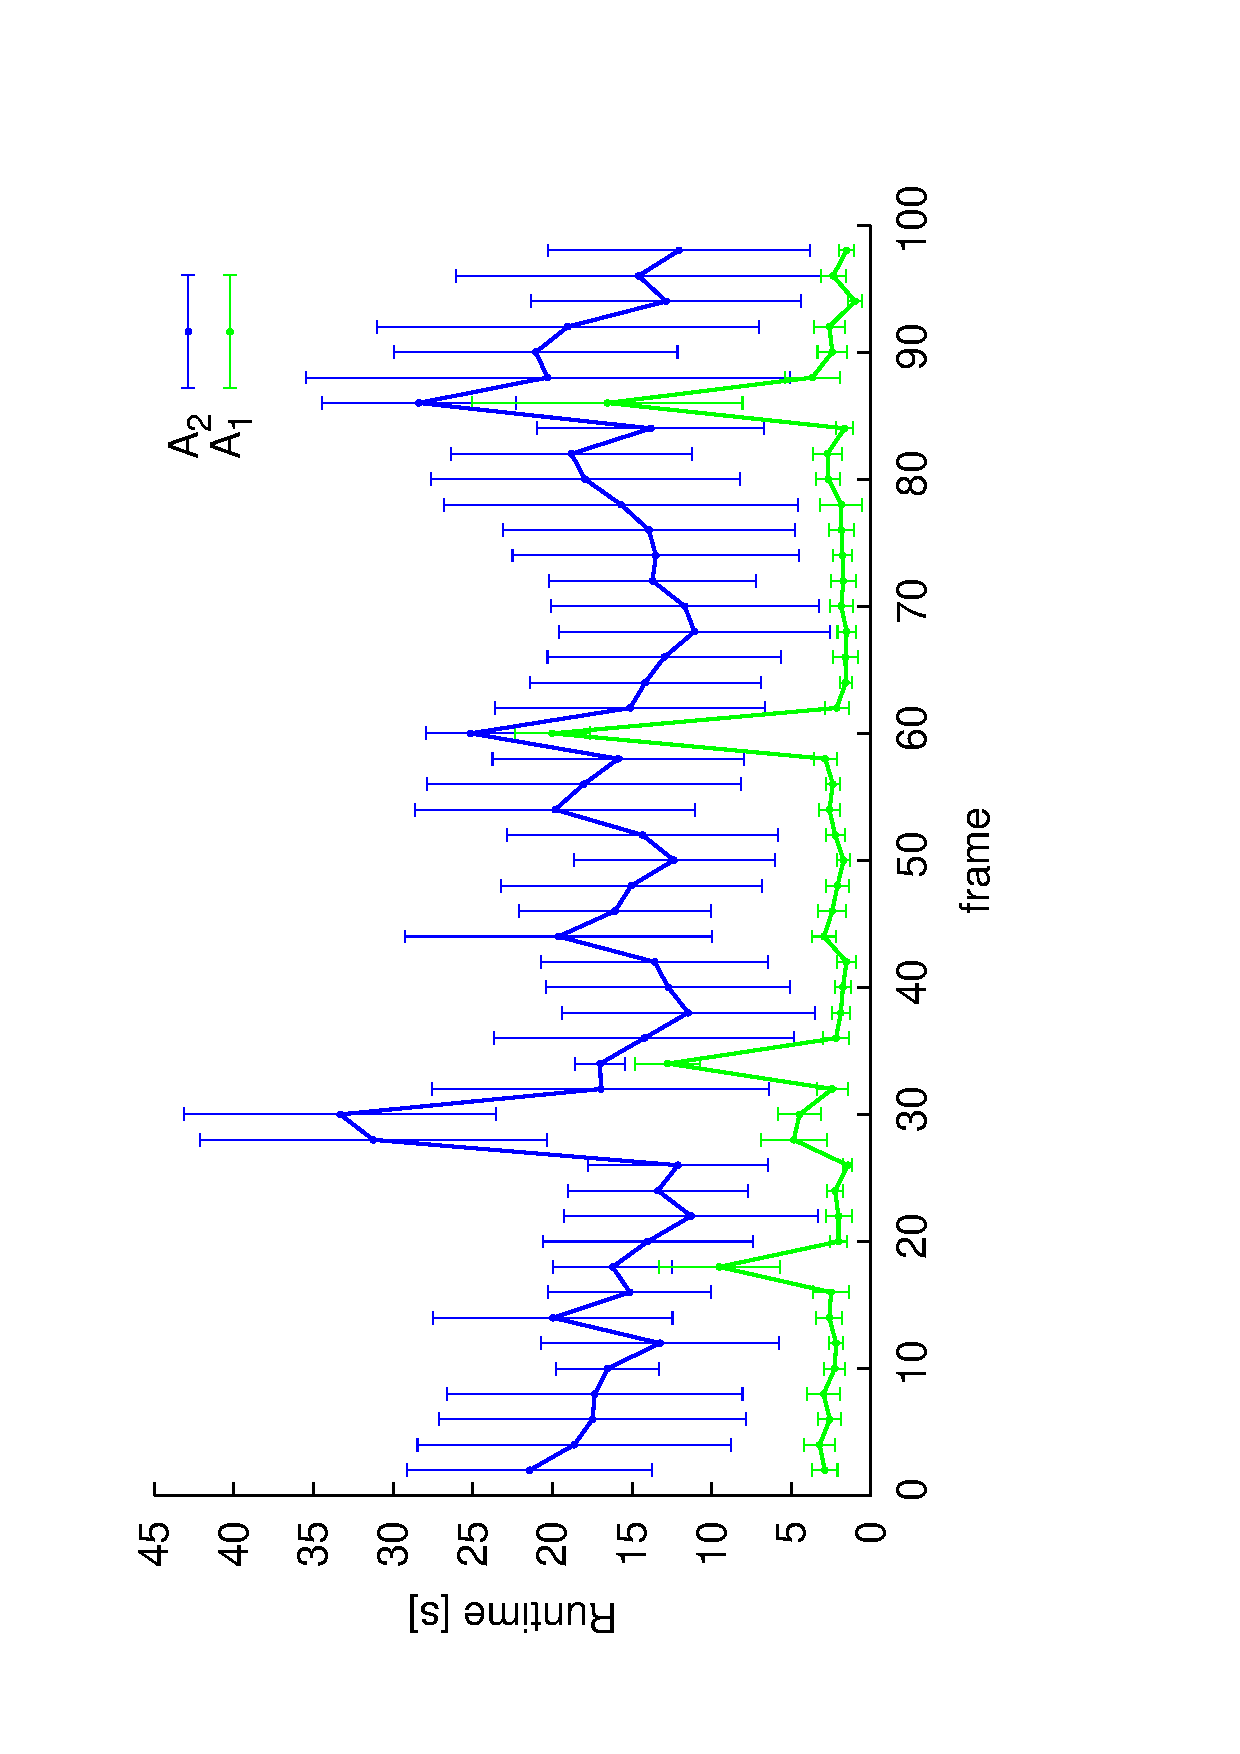
\includegraphics[width=0.25\textwidth,angle=\a]{fig/m037tmins-03tunnel-1rrt_path_time-2}
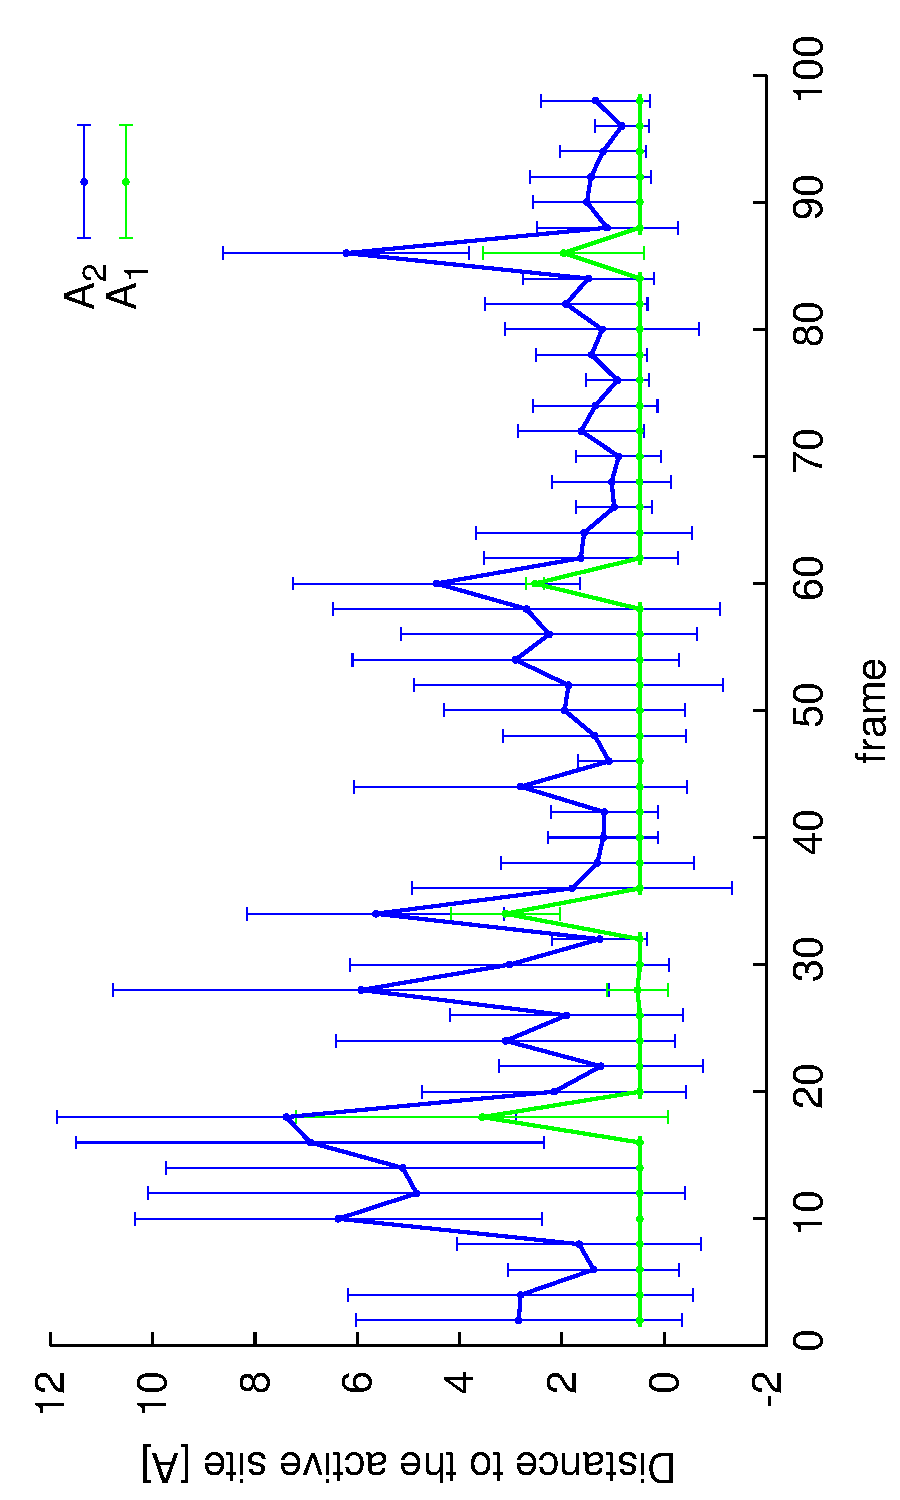
\includegraphics[width=0.25\textwidth,angle=\a]{fig/m037tmins-03tunnel-1trajDistToGoal-2}
\caption{\label{fig::comparison}
    Runtimes and distance to the active site for the m037 ligand at scale 0.6.
    The values are computed from all 200 trials (20 initial configurations $\times$ 10 trials).
    Only each second frame is shown in the graph.
}
\end{figure}
}


\begin{figure}
\centering
\includegraphics[width=0.4\textwidth]{fig/dcp-image1Label}\\
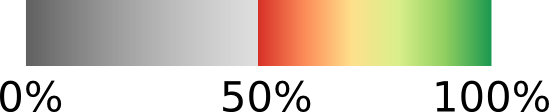
\includegraphics[width=0.2\textwidth]{fig/colormap}
\caption{\label{fig::dcp}
Visualization of trajectories for the ligand DCP   in the two examined tunnels.  
The color of the trajectories corresponds to the scale, that was needed to pass the given part of the tunnel.
The ligand can enter the first tunnel with a high scale (almost 1=100~\%) (A), but then it has to scale-down (to $\sim75$~\%) to pass the
next part of the tunnel (B). After this narrow passage, the tunnel is larger and the ligand can traverse to the narrow passage with
scale $>75$~\% (C).
The second tunnel can also be entered with the high scale (green), but then the narrow part is traversable only with a low scale ($\sim50$~\%) (D). 
For the purpose of the visualization, even more scale-down to 0.3=30~\% was allowed (E) to see how the ligand pass the tunnel.
However, the ligand can reach the active site only with very low scale ($\sim0.4=40$~\%) using the second tunnel.
}
\end{figure}


\section{Discussion and utilization of the results}

The work in the paper is motivated by real needs of bio-chemists who need to analyze traversability of selected ligands in the tunnels.
To enable finding the trajectories, it is necessary to shrink the atomic radii of the ligands which has been utilized also in other tools~\cite{cortes2005path,guieysse2008structure}.
Finding trajectories for scaled-down ligands on one hand helps to cope with the narrow passages, but the question is, how realistic
such trajectories are.

Judging the accessibility of the active sites by the ligands based only on the traversability rates may be problematic if the ligands are scaled too much.
Instead of using a single version of the scale-down ligand, we only limit the minimal scale used by the planner (the parameter $\smin$).
The expansion step always prefers to expand the tree with the maximal scale, that leads to a new collision-free configuration.
The information about the scales used at the trajectory points (which can be extracted from the configuration tree of the proposed planner) brings the chemists new knowledge about the tunnels.
It allows them to detect parts of the tunnels, where the ligand has to scale-down significantly, and parts, where the ligand can be again
larger (Fig.~\ref{fig::dcp}).
According to the results of the motion planinng, DCP needs to shrink down to ca. 75~\% of its size (Fig.~\ref{fig::dcp}, point B).
However, as both the protein and the ligand adapt to each other, it is possible, that even a narrow part of the tunnel is traversable.
This was observed in the MD simulation of the DCP ligand in the 1CQW protein, which revealed that DCP can pass the first tunnel.

%The computed trajectories cannot be considered as `real', they should rather be considered as a hint for the biochemists.
%One of the reason is that the trajectories are computed inside a static protein and static tunnels.
%Real proteins are dynamic structures and consequently also the tunnels are dynamic: they move, merge or even disappear due to motions of protein atoms.
%Contrary, usually static tunnels are used in protein engineering.
%Despite such a simplification, researches often used information about the static tunnels  to estimate the possibility of chemical reactions
%at the active sites.
%The second limitation is caused by the utilization of scaled-down ligands.
%The protein atoms fill the internal void space therefore the tunnels identified inside proteins without ligand tend
%to be very narrow.
%To enable at least some motion of the ligands inside such narrow tunnels, the scaling-down of the ligand atoms is necessary.
%It is used also in other related tool, e.g.~\cite{cortes2005path}.

%Due to these reasons, the computed trajectories can be considered either as too optimistic
%(e.g. because they are computed on a wide tunnel that can be in fact closed due to molecular dynamics),
%or too pessimistic (e.g. the trajectory is not found because of narrow passage around the tunnel, which can be  opened due to the molecular dynamics).
%Despite these limitations, testing the tunnel traversability using motion planning technique can provide chemists more information
%than the simple bottleneck radius, which is used nowadays.
%For example, possible detours from the tunnel can be identified, which indicates that even a tunnel with a small
%bottleneck can be traversed (Fig.~\ref{fig::detail}).

%Most related works, e.g. those based on motion planning, are usually focused on protein folding, or finding arbitrary pathways
%from proteins~\cite{cortes2010simulating,guieysse2008structure}.


%The runtime of the planner is currently given mainly by the collision-detection.
%As the ligand is assumed to travel only along the tunnel centerline (in the distance defined by $\rv$),
%only atoms located in the vicinity of the tunnel can be considered for collision detection.
%Fast collision-detection can be achieved either using fast hierarchical data structures as OBB (implemented, e.g., in~\cite{ozcollide})
%    or using collision-detection system developed directly for proteins~\cite{ruiz2005biocd}.
%We assume that a conformation $l \in \L$ can be switched to all other conformations in $\L$.

%parmas:
%$\RI$
%$\rv$
%$\dt$
%The presented expansion procedure favors the samples with maximal scale (they are tested first), the trajectory contains samples with higher scales at the easy part of the tunnels (e.i., wide areas), and the smaller scales are used only if the ligand has to fit into a narrow space.



\section{Conclusion}

In this paper, we presented a modification of the RRT planner for trajectory computation of ligands inside protein tunnels.
The tunnels are pathways leading from an outer environment toward the active sites, where chemical interactions may undergo.
So far, the tunnels have been detected using Voronoi diagrams, which does not take into account shape of the ligand neither the possible 
conformation changes.
In the proposed work, we compute trajectories using modified RRT for whole ligands and we model the conformation changes of the
ligands using a predefined set of conformations.
The atomic radii of the ligands can be scaled down up to a certain predefined factor.
The planner generates the random samples along a tunnel computed by Voronoi diagram and it attempts to expand the configuration
tree using all conformations. 
The expansion prefers atoms with a higher scale, which ensures that the ligand shrinks down only if traversing narrow parts of the tunnels.
To further boost exploration of the configuration space, a novel metric suitable for measuring distances between various shapes
of the ligands, is used in the expansion step.
The proposed method has been used to  evaluate trajectories of several ligands in a sequence of protein dynamics.
Traversability of one of the tested ligands has been already approved in MD simulations.

\bibliographystyle{plain}
\bibliography{paper}

\end{document}



% ============  unused ideas =========================

%neni treba \cite{cheng01reducing}
%Using a library of predefined conformations has been used also in other tasks, e.g.~\cite{kellogg}.
%This shrinking technique is also used in the MoMa-LigPath tool~\cite{cortes2005path}, which utilizes RRT to find pathways for unbinding a ligand  from a protein.
%It is necessary to use an apporpriated distance metric in the configuration space.
%Generally, it is hard to combine the translational and rotational components in the configuration space.
%In~\cite{zhangRetraction}, the DISP metric~\cite{zhang2008fast}.
%energetic constraints are translated into geometric ones by considering a steric model of the molecules and applying collision detection
%\cite{deAngulo2005biocd}
%First the biredge test is applied to identify regions aeround narrow passages, optimization-based retraction operatoin sleectively only at those regions selective rrt~\cite{lee2012srrrt}
%Free-space dilation is an effective aproach for narrow passage sampling~\cite{hsu06multilevel}. 
%It is necessary to define proper method for dilating and determin the amount of dilation.
%\cite{saha2005finding}
%DISP metric \cite{zhang2008fast}


\subsection{Traversability Characteristics}

For each initial configuration $\qinit \in \QI$, $K$ trajectories are computed, which results in the set of $K |\QI|$ trajectories.
All these trajectories are used to compute the following properties of the tunnel $T$.
A trajectory $P$ reaches the tunnel sphere $c_i \in T$, if the 3D Euclidean distance of the 
nearest configuration $q \in P$ towards $c_i$ is less than $r_i$ (radius of the sphere $c_i$).
Let $N(i)$ denote the number of trajectories that reached $i-$th sphere of the tunnel, $i=1,\ldots,n$.
Three basic characteristics of the tunnel are computed from the trajectories: accessibility, throughput, and the scaling factor.

The accessibility $A(i)=N(i)/N$ of the sphere $i$ is the probability of reaching the sphere $i$, where $N=K|\QI|$ is the total number of trajectories.
The accessibility shows how probable it is to pass the tunnel up to the sphere $i$.
Obviously, the most important is $A(n)$ of the last sphere of the tunnel, which can be considered as the overall difficulty of the tunnel.
The  ligand passage may however be strongly affected by the first bottleneck, so the parts of the tunnel located behind
the bottleneck have low accessibility.

The throughput $T(i)$ is the ratio of trajectories that passed sphere $i$ (i.e., visited sphere $i+1$) and reached the sphere $i$,
i.e., $T(i) = N(i+1) / N(i)$. 
The throughput is not computed for the last sphere ($i=N$).
The throughput shows a local accessibility of tunnel parts and it can be used to detect places where most of the trajectories ends.

The proposed planner is allowed to scale down the radii of ligand spheres up to the allowed scale $\smin$. 
It can be expected that narrower parts of the tunnel are more often passed with a more scaled-down ligand than
the wider parts.
Ligand scale $L(i)$ at the tunnel sphere $i$ is the average scale of ligand that reaches the sphere $i$.


\begin{figure}
\centering
{
\renewcommand{\tabcolsep}{-5pt}
\begin{tabular}{ccc}
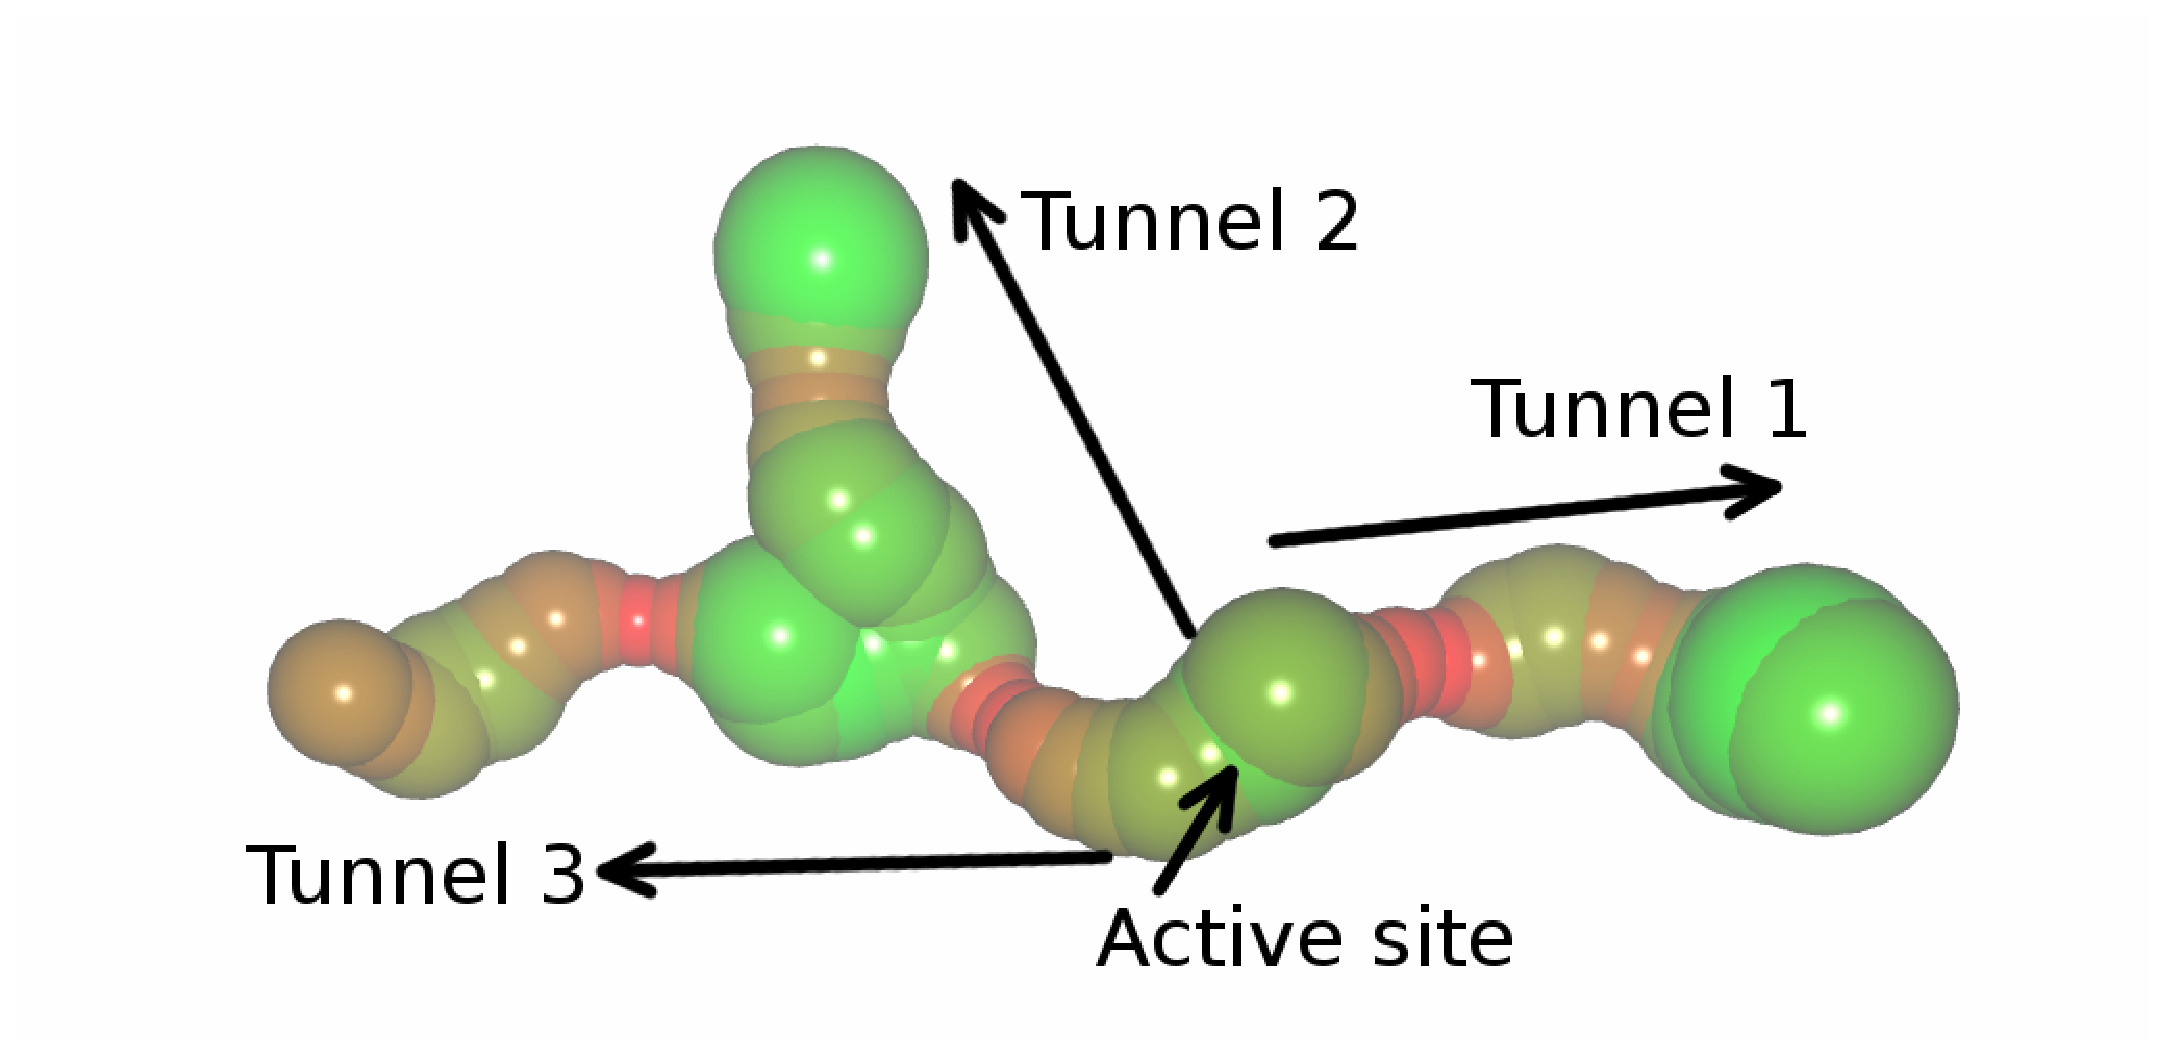
\includegraphics[width=0.38\textwidth]{fig/t05proteinBottle2T} & 
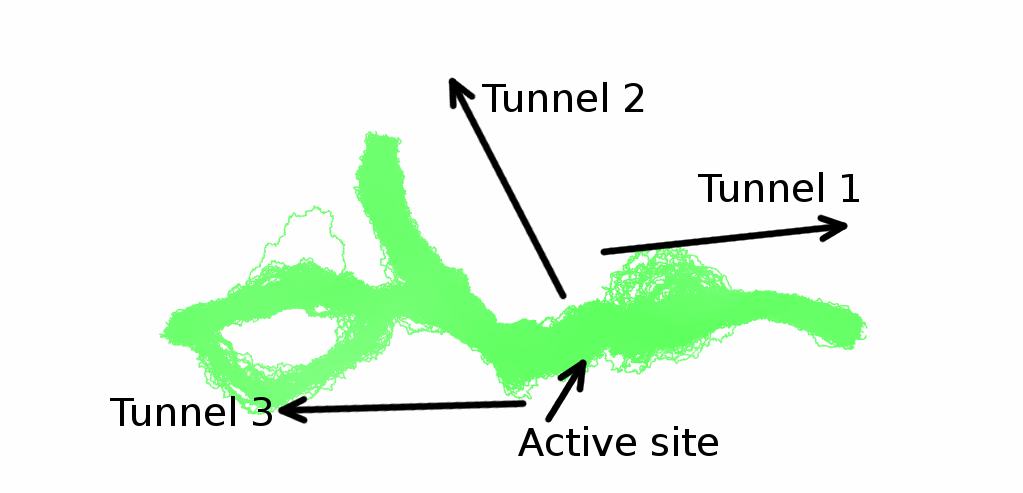
\includegraphics[width=0.38\textwidth]{fig/t04goodT} & 
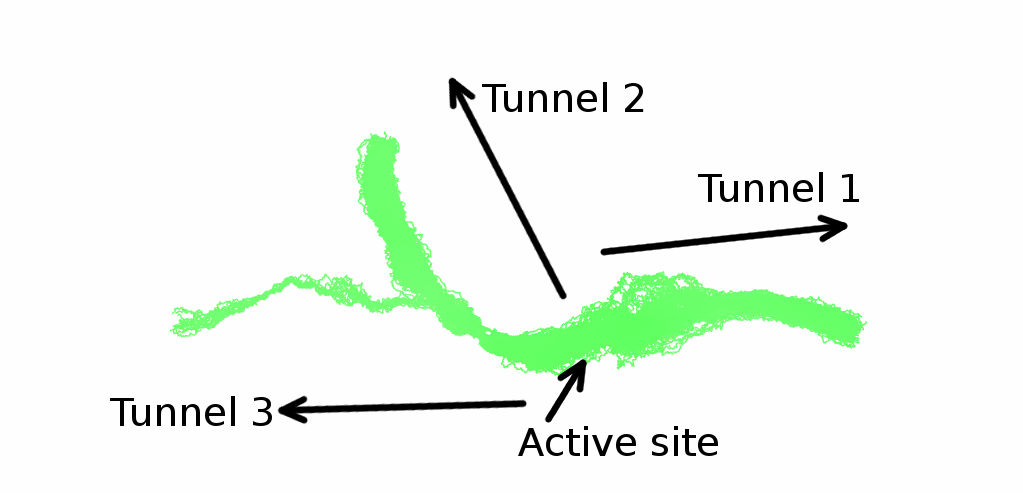
\includegraphics[width=0.38\textwidth]{fig/t05goodT} \\
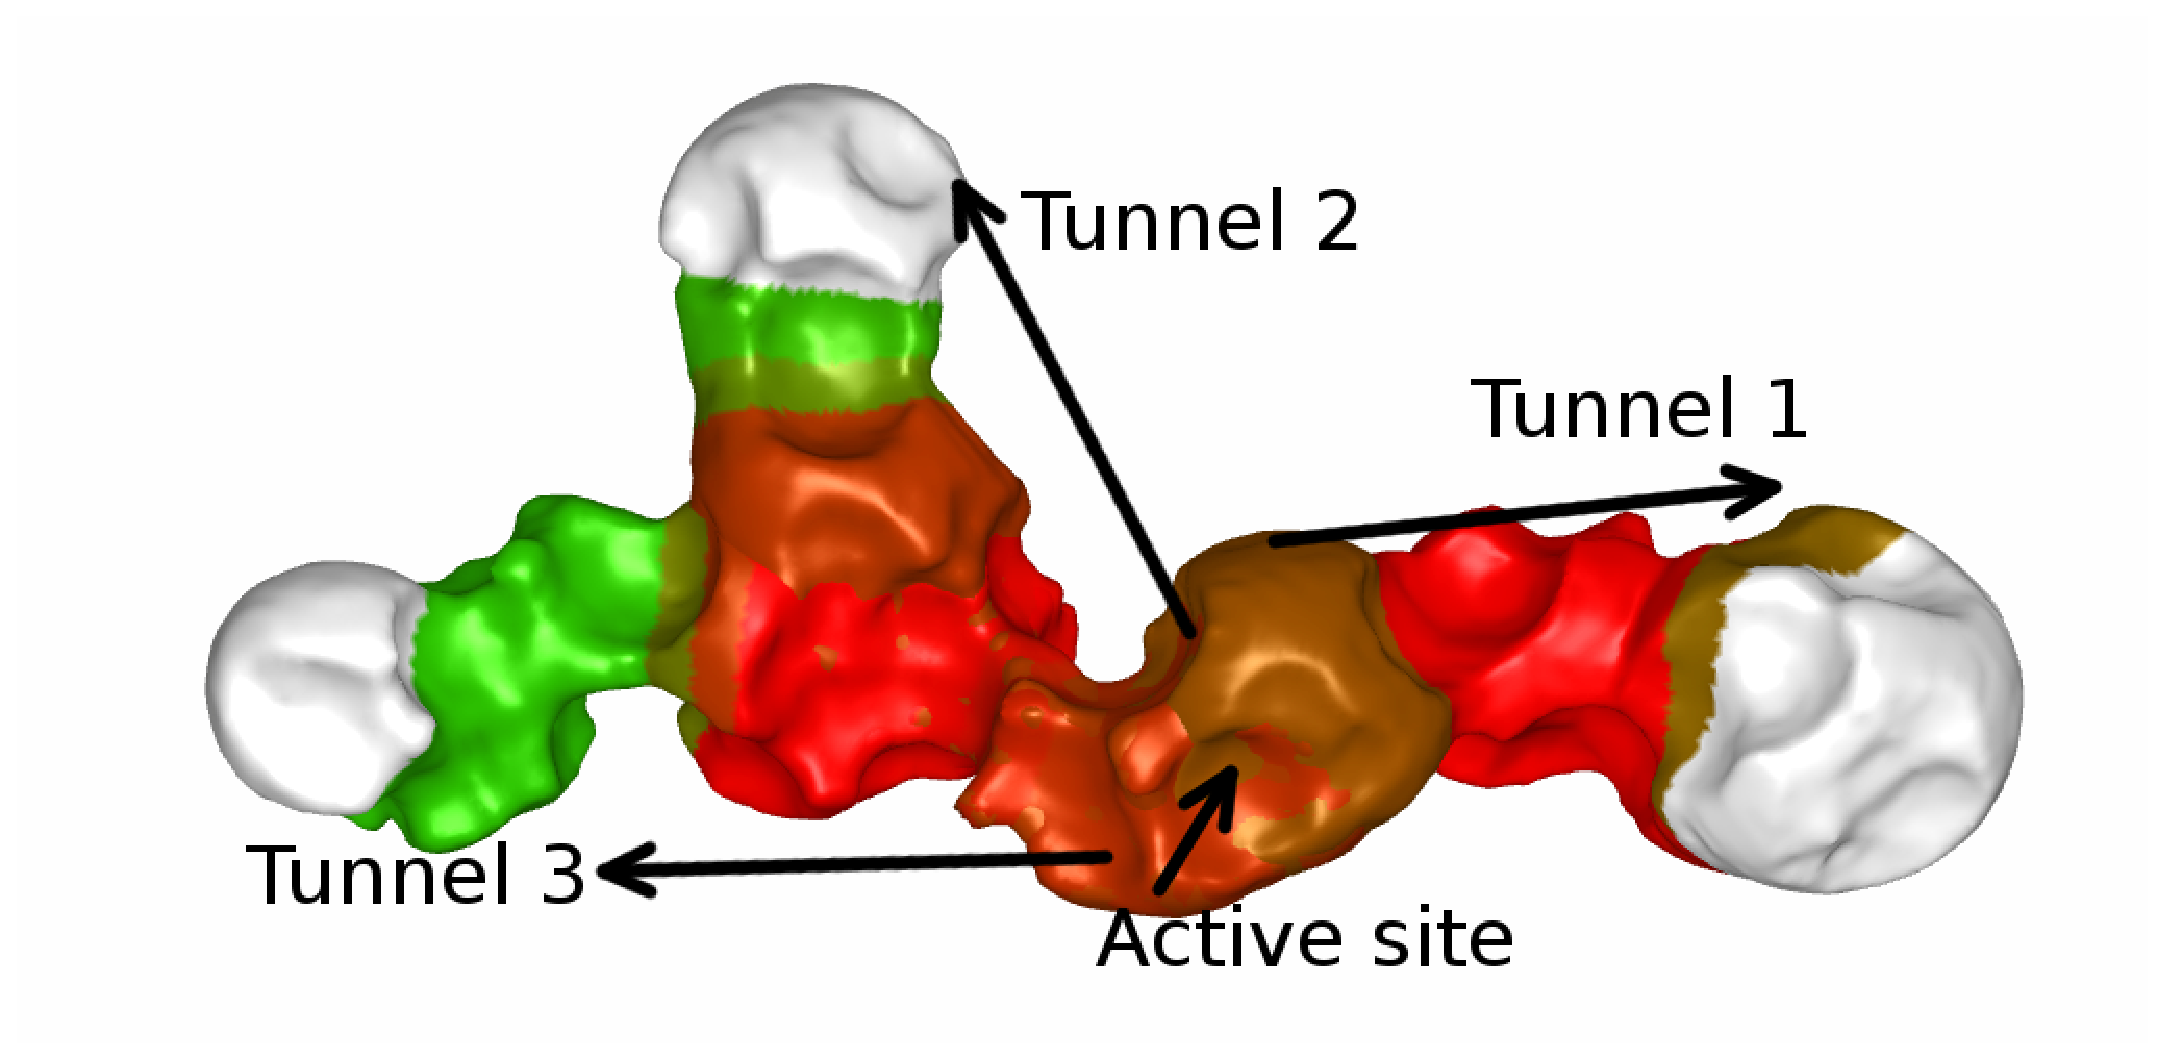
\includegraphics[width=0.38\textwidth]{fig/t05thpT} &
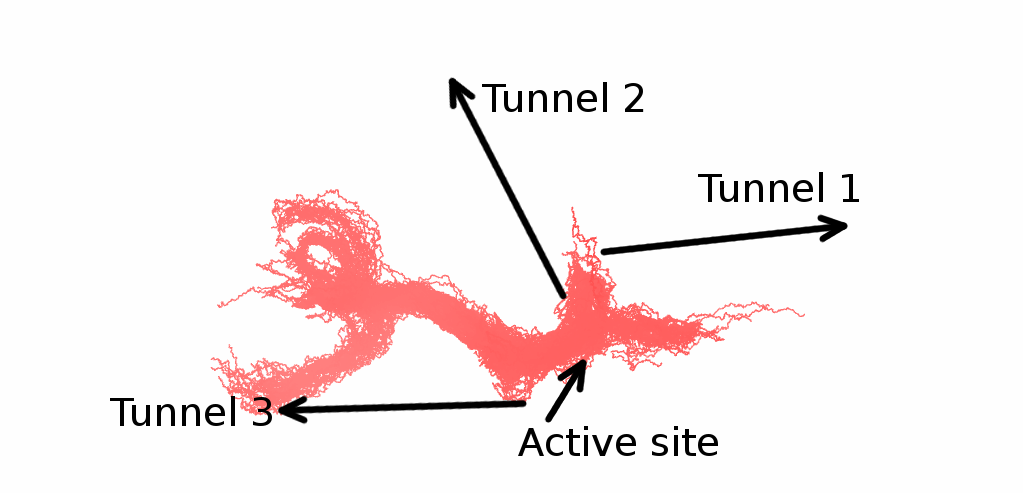
\includegraphics[width=0.38\textwidth]{fig/t04badT} &
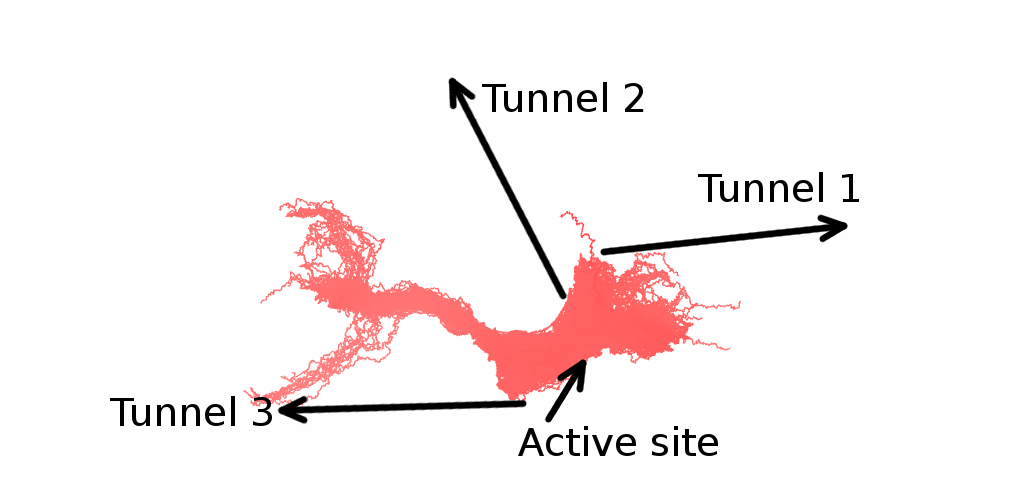
\includegraphics[width=0.38\textwidth]{fig/t05badT} \\ 
(a) & (b) & (c)                       
\end{tabular}                       
\caption{\label{fig::tunnel2}
    (a) Classic bottleneck for spherical probe (top) and visualization of throughput (bottom) for the ligand $\LA$.
    (b) Successful (green, top) trajectories that reached end points of the tunnels,
        and unsuccessful ones (red, bottom) for $\smin=0.4$.
    (c) Successful and unsuccessful trajectories for $\smin=0.5$.
}
}
\end{figure}


\begin{figure}
\centering
{
\renewcommand{\tabcolsep}{0pt}
\begin{tabular}{ccc}
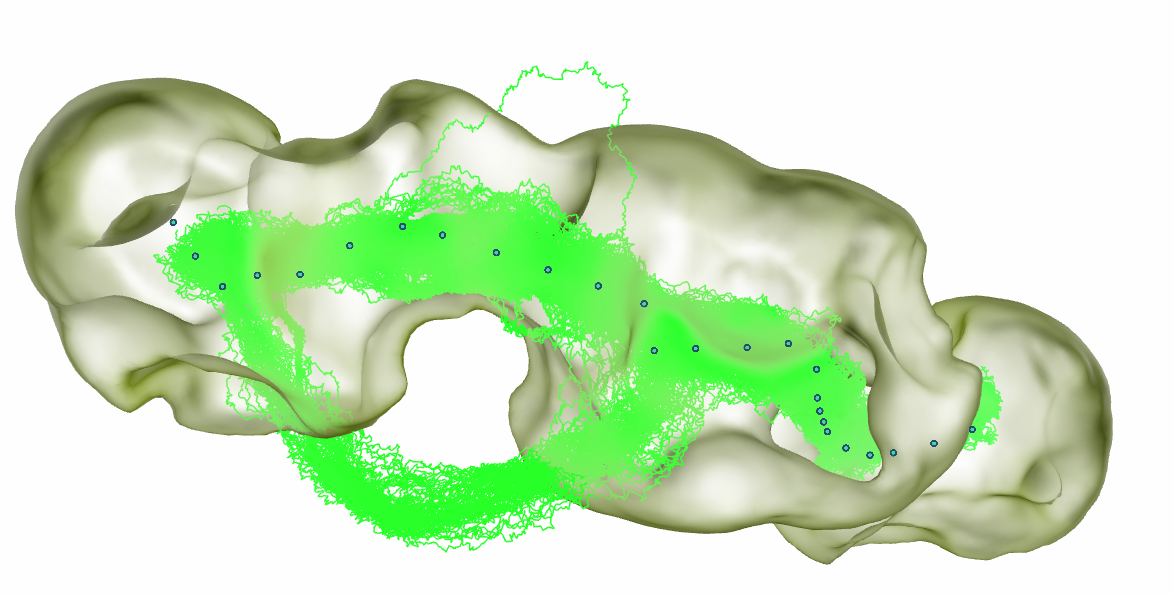
\includegraphics[width=0.325\textwidth]{fig/tunne4ac}& 
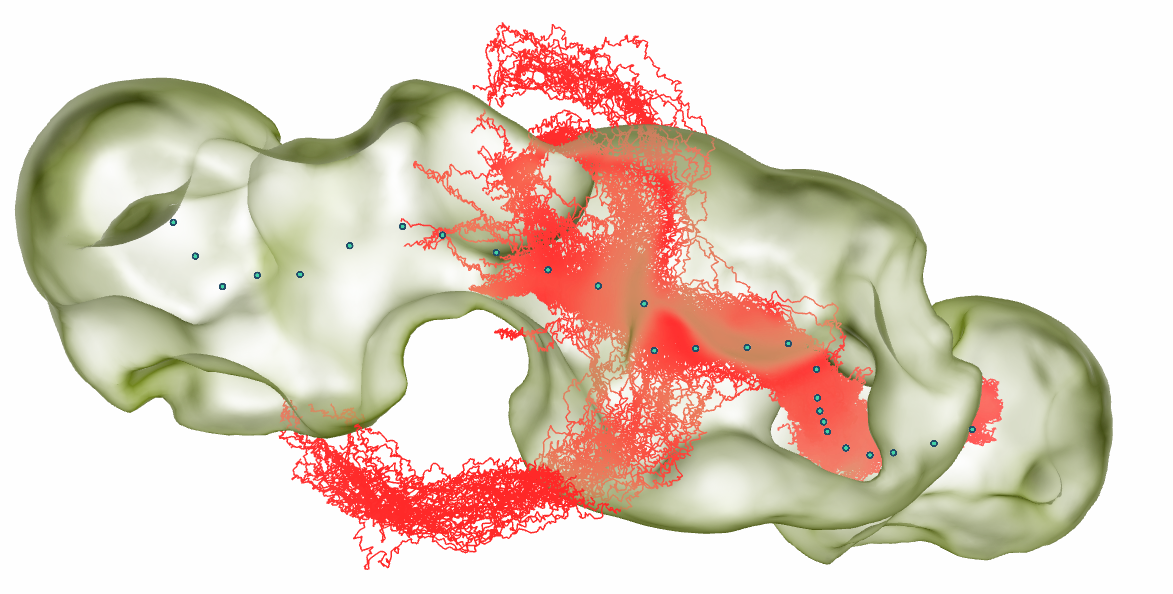
\includegraphics[width=0.325\textwidth]{fig/tunne4bc} & 
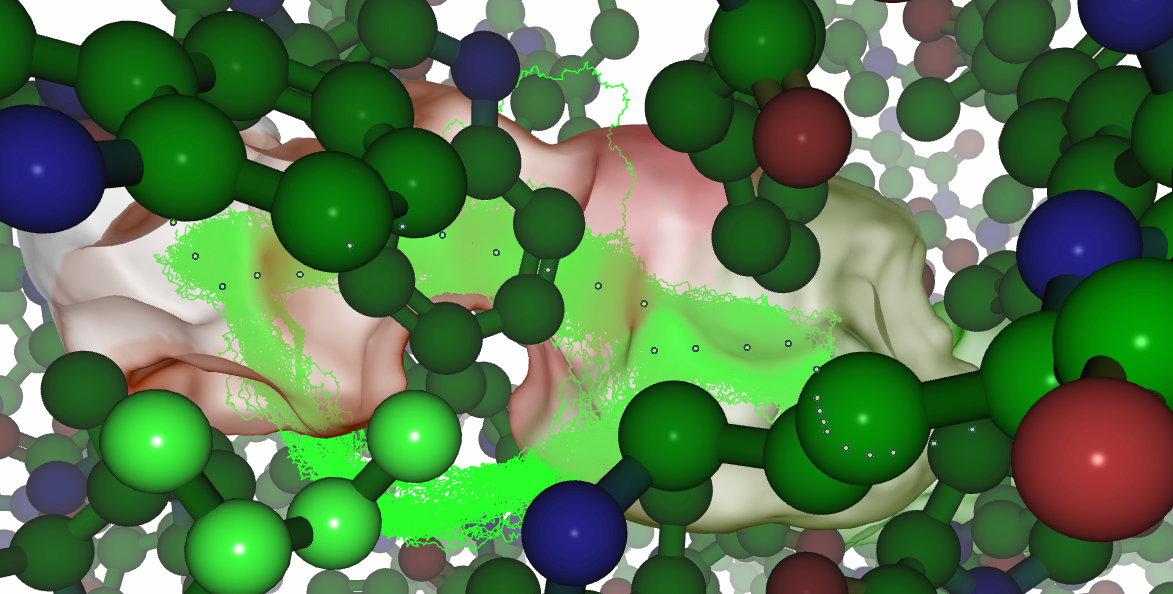
\includegraphics[width=0.325\textwidth]{fig/tunne4cc} \\
(a) & (b) & (c)                        
\end{tabular}
}
\caption{\label{fig::detail}
    Detailed view to alternative pathway around the third tunnel in 1CQW.
    The successful trajectories are in green (a) the unsuccessful in red (b).
    (c) Shows visualization of protein atoms around the tunnel.
}
\end{figure}


Besides the color mapping, it is also necessary to show the computed trajectories.
%This is useful, for example, to find out in which part of the tunnel the trajectories detour.
Simple visualization of all trajectories could however be too slow for an interactive work.
Therefore, the trajectories are first clustered and then only the clusters are visualized.
Due to different lengths of the trajectories, they are first converted to a normalized form.
Let $\cstart$ represent the average starting position of all trajectories and let $d_{max}$ be the 3D Euclidean distance
of the most distant configuration from $\cstart$ among all trajectories.
A set of $M$ spheres centered at $\cstart$ are created with radii $r'_i=i {d_{max} \over M}$, where $i=0,\ldots, M-1$.
The trajectory $P=(q_1,\ldots,q_n)$ of length $n$ is represented by the normalized vector $v=(x_1,\ldots,x_M)$ of length $M$,
where $x_i$ is the 3D position of the nearest configuration $q \in P$ to the surface of the $i$-th sphere with the radius $r'_i$.
The distance between two normalized trajectories $v_i$ and $v_j$ is defined as
$d(v_i, v_j) = \frac{1}{M} \sum_{1 \leq k \leq N} |x_k^i x_k^j|$.
This distance is used in the UPGMA clustering technique~\cite{sokal1958statistical}.
The trajectories can be visualized using a representative of each cluster.
The number of trajectories in each cluster is represented by the width of the polyline (Fig.~\ref{fig:trajectories}).
%In this manner, we are able to convey the information about all different trajectories together (see Fig.~\ref{fig:trajectories} right).


\begin{figure}
\centering
\begin{tabular}{cc}
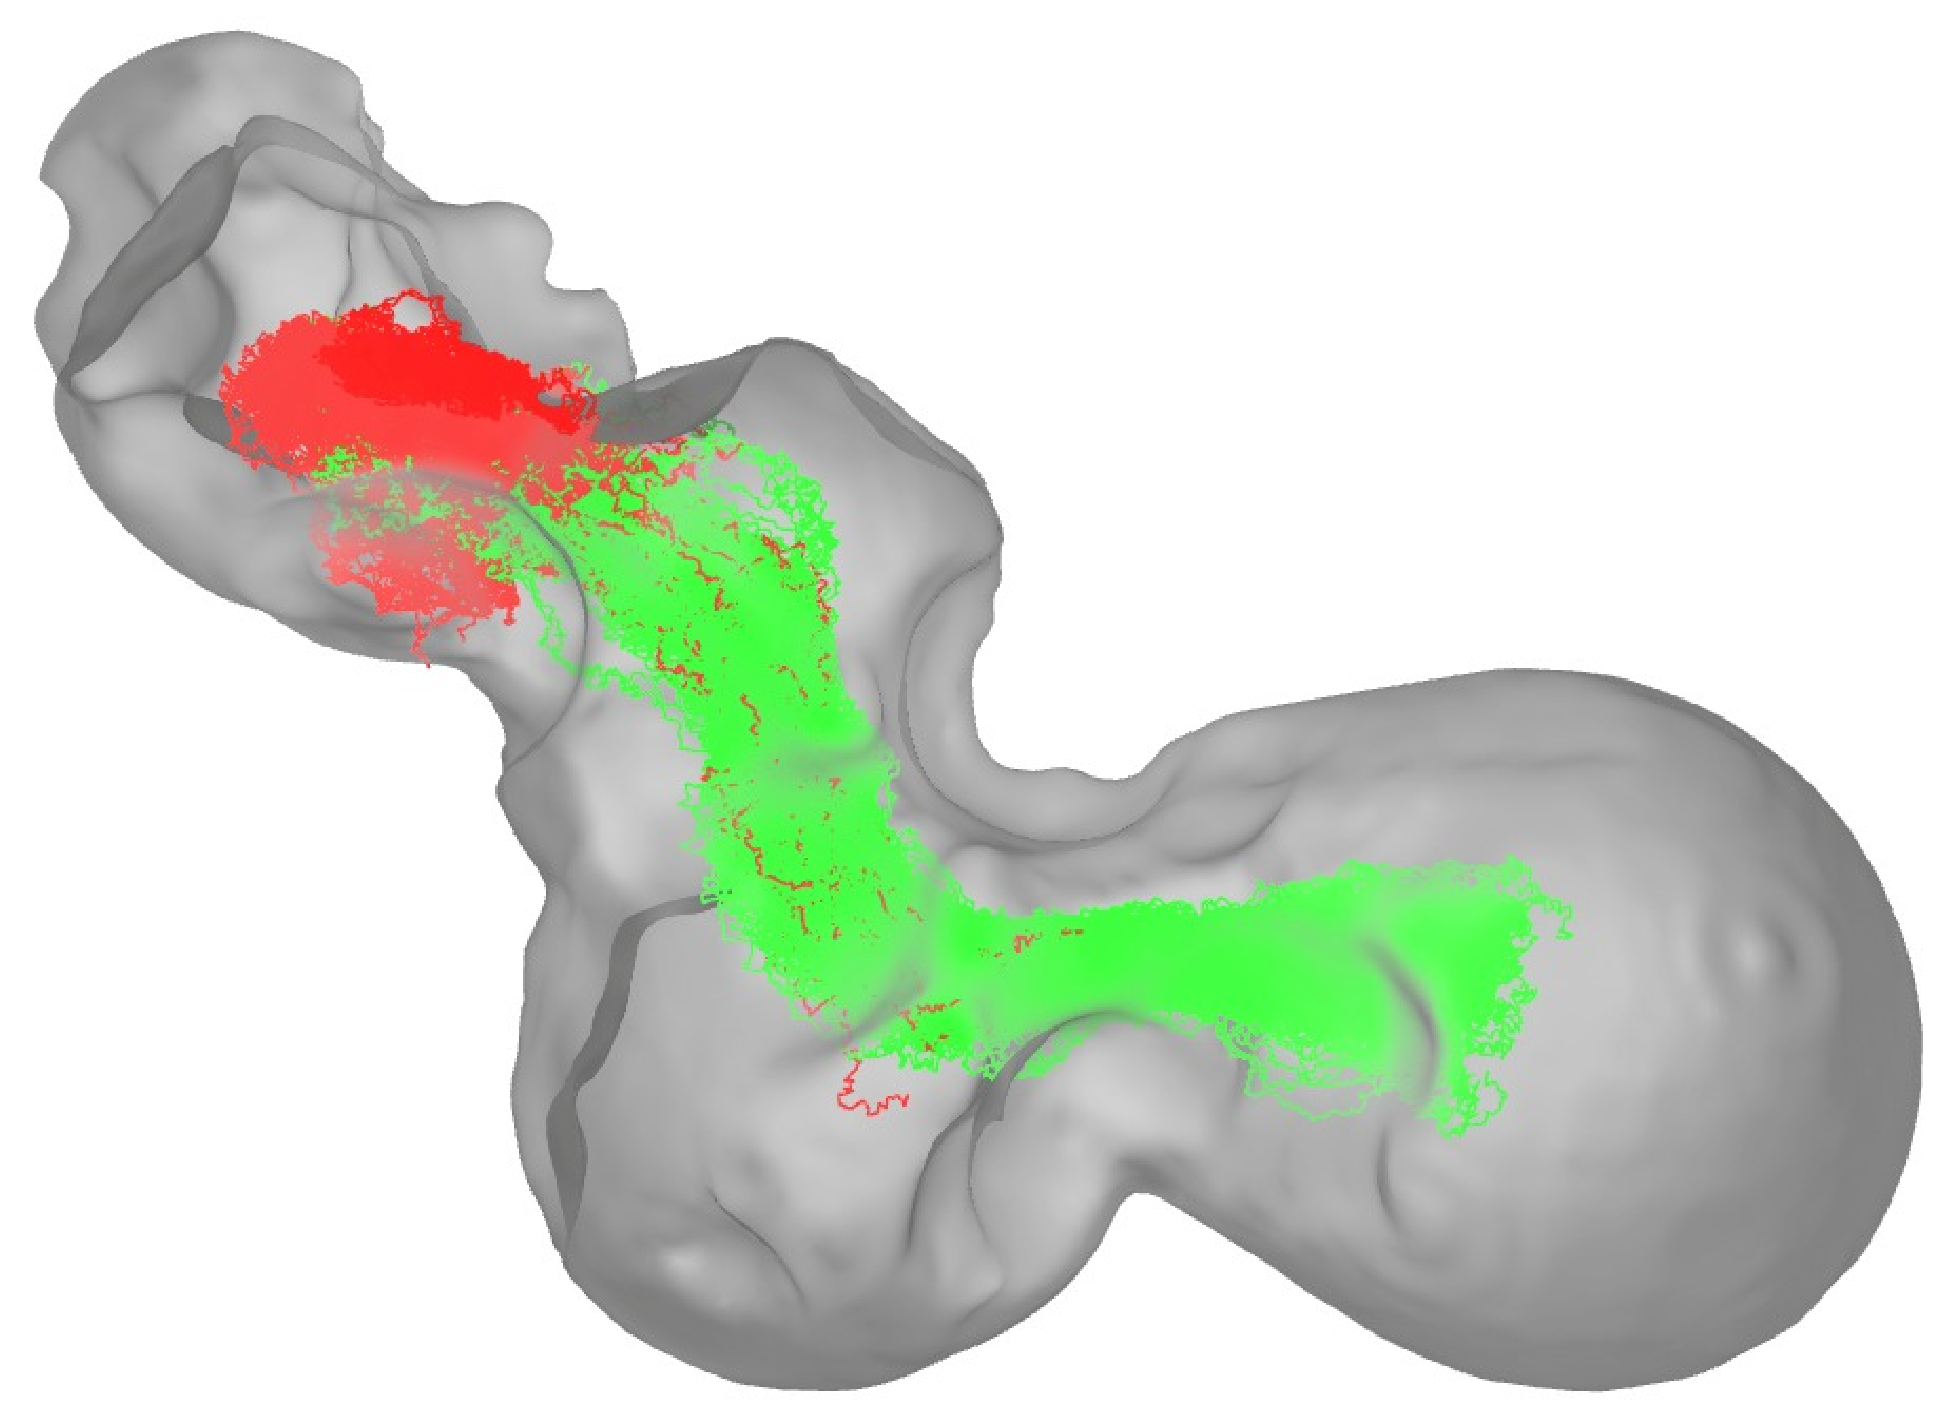
\includegraphics[width=0.4\textwidth]{fig/trajectories-all} &
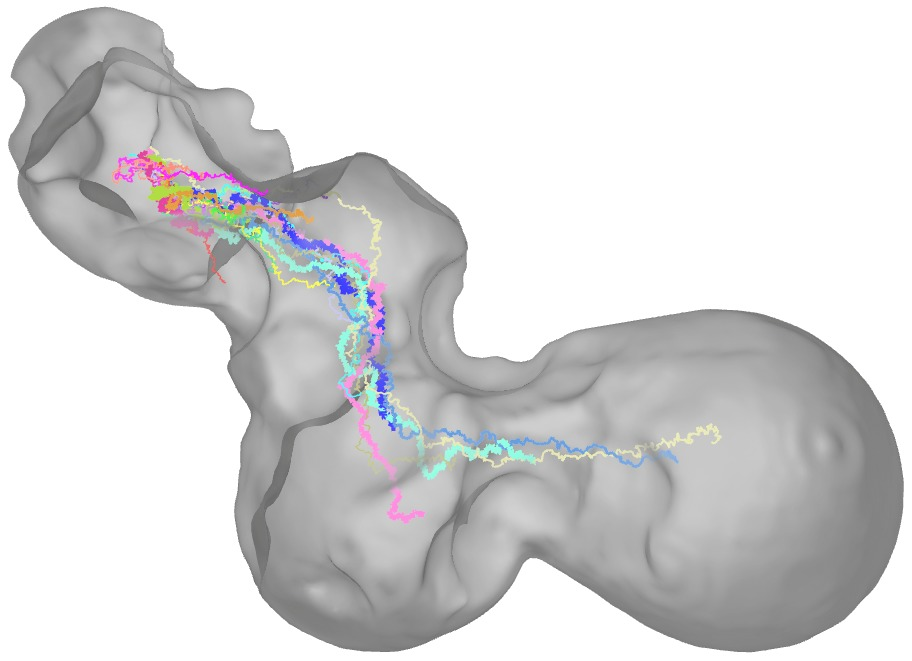
\includegraphics[width=0.4\textwidth]{fig/trajectories-clustered-21} \\
(a) & (b) \\                       
\end{tabular}
\caption{Visualization of the trajectories. The tunnel begins in the top left corner.
(a) All trajectories ($\sim5000$) colored according to whether they reached the end of the tunnel (green) or not (red). 
(b) Visualization using clusters of trajectories. 
%Trajectories clustered according to their proximity colored by distinct colors.
%The different line widths represent the number of trajectories in a cluster.
\label{fig:trajectories}
}
\end{figure}



\begin{table}
\centering
\caption{\label{tab::rrt}
    Runtime and success ratio for ligand $\LA$ (left) and $\LB$ (right).
}
{
\small
\renewcommand{\tabcolsep}{1pt}
\input table.003.tex
\hskip 4pt   
\input table.004.tex
}
\end{table}


Trajectories for $\LA$ in all detected tunnels were classified as successful if they reached the last sphere of the tunnel
to distance $\dt=2$~\AA and they were considered unsuccessful otherwise.
The throughput computed from the trajectories shows that the tunnels are difficult not only around bottlenecks, but
also in other places.
The comparison of the classic bottleneck (i.e., measured by the radius of spherical probe) and throughput is depicted in Fig.~\ref{fig::tunnel2}a.
The trajectories for $\smin=0.4$ are depicted in Fig.~\ref{fig::tunnel2}b and for $\smin=0.5$ in Fig.~\ref{fig::tunnel2}c.
The successful trajectories for $\smin=0.4$ reveal that the end of the tunnel No. 3 can be approached by two different pathways (one in the tunnel and another one outside the tunnel).
The detail is depicted in Fig.~\ref{fig::detail}.
Despite the low bottleneck of this tunnel, the ligand may reach its end using the alternative pathway. 



